\documentclass[twoside]{book}

% Packages required by doxygen
\usepackage{calc}
\usepackage{doxygen}
\usepackage{graphicx}
\usepackage[utf8]{inputenc}
\usepackage{makeidx}
\usepackage{multicol}
\usepackage{multirow}
\usepackage{textcomp}
\usepackage[table]{xcolor}

% Font selection
\usepackage[T1]{fontenc}
\usepackage{mathptmx}
\usepackage[scaled=.90]{helvet}
\usepackage{courier}
\usepackage{amssymb}
\usepackage{sectsty}
\renewcommand{\familydefault}{\sfdefault}
\allsectionsfont{%
  \fontseries{bc}\selectfont%
  \color{darkgray}%
}
\renewcommand{\DoxyLabelFont}{%
  \fontseries{bc}\selectfont%
  \color{darkgray}%
}

% Page & text layout
\usepackage{geometry}
\geometry{%
  a4paper,%
  top=2.5cm,%
  bottom=2.5cm,%
  left=2.5cm,%
  right=2.5cm%
}
\tolerance=750
\hfuzz=15pt
\hbadness=750
\setlength{\emergencystretch}{15pt}
\setlength{\parindent}{0cm}
\setlength{\parskip}{0.2cm}
\makeatletter
\renewcommand{\paragraph}{%
  \@startsection{paragraph}{4}{0ex}{-1.0ex}{1.0ex}{%
    \normalfont\normalsize\bfseries\SS@parafont%
  }%
}
\renewcommand{\subparagraph}{%
  \@startsection{subparagraph}{5}{0ex}{-1.0ex}{1.0ex}{%
    \normalfont\normalsize\bfseries\SS@subparafont%
  }%
}
\makeatother

% Headers & footers
\usepackage{fancyhdr}
\pagestyle{fancyplain}
\fancyhead[LE]{\fancyplain{}{\bfseries\thepage}}
\fancyhead[CE]{\fancyplain{}{}}
\fancyhead[RE]{\fancyplain{}{\bfseries\leftmark}}
\fancyhead[LO]{\fancyplain{}{\bfseries\rightmark}}
\fancyhead[CO]{\fancyplain{}{}}
\fancyhead[RO]{\fancyplain{}{\bfseries\thepage}}
\fancyfoot[LE]{\fancyplain{}{}}
\fancyfoot[CE]{\fancyplain{}{}}
\fancyfoot[RE]{\fancyplain{}{\bfseries\scriptsize Generated on Thu Mar 9 2017 17\-:50\-:54 for My Project by Doxygen }}
\fancyfoot[LO]{\fancyplain{}{\bfseries\scriptsize Generated on Thu Mar 9 2017 17\-:50\-:54 for My Project by Doxygen }}
\fancyfoot[CO]{\fancyplain{}{}}
\fancyfoot[RO]{\fancyplain{}{}}
\renewcommand{\footrulewidth}{0.4pt}
\renewcommand{\chaptermark}[1]{%
  \markboth{#1}{}%
}
\renewcommand{\sectionmark}[1]{%
  \markright{\thesection\ #1}%
}

% Indices & bibliography
\usepackage{natbib}
\usepackage[titles]{tocloft}
\setcounter{tocdepth}{3}
\setcounter{secnumdepth}{5}
\makeindex

% Hyperlinks (required, but should be loaded last)
\usepackage{ifpdf}
\ifpdf
  \usepackage[pdftex,pagebackref=true]{hyperref}
\else
  \usepackage[ps2pdf,pagebackref=true]{hyperref}
\fi
\hypersetup{%
  colorlinks=true,%
  linkcolor=blue,%
  citecolor=blue,%
  unicode%
}

% Custom commands
\newcommand{\clearemptydoublepage}{%
  \newpage{\pagestyle{empty}\cleardoublepage}%
}


%===== C O N T E N T S =====

\begin{document}

% Titlepage & ToC
\hypersetup{pageanchor=false}
\pagenumbering{roman}
\begin{titlepage}
\vspace*{7cm}
\begin{center}%
{\Large My Project }\\
\vspace*{1cm}
{\large Generated by Doxygen 1.8.6}\\
\vspace*{0.5cm}
{\small Thu Mar 9 2017 17:50:54}\\
\end{center}
\end{titlepage}
\clearemptydoublepage
\tableofcontents
\clearemptydoublepage
\pagenumbering{arabic}
\hypersetup{pageanchor=true}

%--- Begin generated contents ---
\chapter{Namespace Index}
\section{Namespace List}
Here is a list of all documented namespaces with brief descriptions\-:\begin{DoxyCompactList}
\item\contentsline{section}{\hyperlink{namespaceenumerator}{enumerator} \\*Class to store Enumerators used in the project }{\pageref{namespaceenumerator}}{}
\end{DoxyCompactList}

\chapter{Hierarchical Index}
\section{Class Hierarchy}
This inheritance list is sorted roughly, but not completely, alphabetically\-:\begin{DoxyCompactList}
\item \contentsline{section}{Jumping\-State}{\pageref{classJumpingState}}{}
\begin{DoxyCompactList}
\item \contentsline{section}{Is\-Jumping}{\pageref{classIsJumping}}{}
\item \contentsline{section}{Is\-Not\-Jumping}{\pageref{classIsNotJumping}}{}
\end{DoxyCompactList}
\item \contentsline{section}{Keys}{\pageref{classKeys}}{}
\item Q\-Graphics\-Pixmap\-Item\begin{DoxyCompactList}
\item \contentsline{section}{Button}{\pageref{classButton}}{}
\item \contentsline{section}{Gem}{\pageref{classGem}}{}
\begin{DoxyCompactList}
\item \contentsline{section}{Diamond}{\pageref{classDiamond}}{}
\end{DoxyCompactList}
\item \contentsline{section}{Graphics\-Component}{\pageref{classGraphicsComponent}}{}
\begin{DoxyCompactList}
\item \contentsline{section}{Fire\-Graphics\-Component}{\pageref{classFireGraphicsComponent}}{}
\item \contentsline{section}{Player\-Graphics\-Component}{\pageref{classPlayerGraphicsComponent}}{}
\end{DoxyCompactList}
\end{DoxyCompactList}
\item Q\-Graphics\-Rect\-Item\begin{DoxyCompactList}
\item \contentsline{section}{Door}{\pageref{classDoor}}{}
\item \contentsline{section}{Tile}{\pageref{classTile}}{}
\end{DoxyCompactList}
\item Q\-Graphics\-Text\-Item\begin{DoxyCompactList}
\item \contentsline{section}{Score\-Component}{\pageref{classScoreComponent}}{}
\item \contentsline{section}{Timer}{\pageref{classTimer}}{}
\end{DoxyCompactList}
\item Q\-Graphics\-View\begin{DoxyCompactList}
\item \contentsline{section}{Input\-Handler}{\pageref{classInputHandler}}{}
\end{DoxyCompactList}
\item Q\-Object\begin{DoxyCompactList}
\item \contentsline{section}{Button}{\pageref{classButton}}{}
\item \contentsline{section}{Choice\-Server\-Client\-Start}{\pageref{classChoiceServerClientStart}}{}
\item \contentsline{section}{Client}{\pageref{classClient}}{}
\item \contentsline{section}{Game\-Object}{\pageref{classGameObject}}{}
\item \contentsline{section}{Game\-State}{\pageref{classGameState}}{}
\item \contentsline{section}{Graphics\-Component}{\pageref{classGraphicsComponent}}{}
\item \contentsline{section}{Input\-Component}{\pageref{classInputComponent}}{}
\begin{DoxyCompactList}
\item \contentsline{section}{Computer\-Input\-Component}{\pageref{classComputerInputComponent}}{}
\item \contentsline{section}{Empty\-Input\-Component}{\pageref{classEmptyInputComponent}}{}
\item \contentsline{section}{Human\-Input\-Component}{\pageref{classHumanInputComponent}}{}
\end{DoxyCompactList}
\item \contentsline{section}{Physics\-Component}{\pageref{classPhysicsComponent}}{}
\begin{DoxyCompactList}
\item \contentsline{section}{Empty\-Physics\-Component}{\pageref{classEmptyPhysicsComponent}}{}
\item \contentsline{section}{Monster\-Physics\-Component}{\pageref{classMonsterPhysicsComponent}}{}
\item \contentsline{section}{Player\-Physics\-Component}{\pageref{classPlayerPhysicsComponent}}{}
\end{DoxyCompactList}
\item \contentsline{section}{Server}{\pageref{classServer}}{}
\end{DoxyCompactList}
\item \contentsline{section}{Read\-Input}{\pageref{classReadInput}}{}
\item \contentsline{section}{State}{\pageref{classState}}{}
\begin{DoxyCompactList}
\item \contentsline{section}{Dead\-Left}{\pageref{classDeadLeft}}{}
\item \contentsline{section}{Dead\-Right}{\pageref{classDeadRight}}{}
\item \contentsline{section}{Moving\-Left}{\pageref{classMovingLeft}}{}
\item \contentsline{section}{Moving\-Right}{\pageref{classMovingRight}}{}
\item \contentsline{section}{Stop\-Left}{\pageref{classStopLeft}}{}
\item \contentsline{section}{Stop\-Right}{\pageref{classStopRight}}{}
\end{DoxyCompactList}
\item \contentsline{section}{Thread\-Pool}{\pageref{classThreadPool}}{}
\end{DoxyCompactList}

\chapter{Class Index}
\section{Class List}
Here are the classes, structs, unions and interfaces with brief descriptions\-:\begin{DoxyCompactList}
\item\contentsline{section}{\hyperlink{classButton}{Button} \\*All the buttons displayed in Main Menu }{\pageref{classButton}}{}
\item\contentsline{section}{\hyperlink{classChoiceServerClientStart}{Choice\-Server\-Client\-Start} \\*The Choice between \hyperlink{classServer}{Server} Client\-Start class }{\pageref{classChoiceServerClientStart}}{}
\item\contentsline{section}{\hyperlink{classClient}{Client} \\*The Class to Create a \hyperlink{classClient}{Client} }{\pageref{classClient}}{}
\item\contentsline{section}{\hyperlink{classComputerInputComponent}{Computer\-Input\-Component} \\*The input component to handle state changes for non human input }{\pageref{classComputerInputComponent}}{}
\item\contentsline{section}{\hyperlink{classDeadLeft}{Dead\-Left} \\*The state in which the player is dead facing left This also handles the responds to key press and key release inputs so as to change the state of the \hyperlink{classGameObject}{Game\-Object} }{\pageref{classDeadLeft}}{}
\item\contentsline{section}{\hyperlink{classDeadRight}{Dead\-Right} \\*The state in which the player is dead facing right This also handles the responds to key press and key release inputs so as to change the state of the \hyperlink{classGameObject}{Game\-Object} }{\pageref{classDeadRight}}{}
\item\contentsline{section}{\hyperlink{classDiamond}{Diamond} \\*Describes a \hyperlink{classDiamond}{Diamond} Handles the drawing, placement on screen, and position of a diamond }{\pageref{classDiamond}}{}
\item\contentsline{section}{\hyperlink{classDoor}{Door} \\*The area which marks the end point of the game The \hyperlink{classDoor}{Door} is an object, which when a player touches, the player completes the game }{\pageref{classDoor}}{}
\item\contentsline{section}{\hyperlink{classEmptyInputComponent}{Empty\-Input\-Component} \\*\hyperlink{classInputComponent}{Input\-Component} for Game\-Objects that do not have any state changes }{\pageref{classEmptyInputComponent}}{}
\item\contentsline{section}{\hyperlink{classEmptyPhysicsComponent}{Empty\-Physics\-Component} \\*\hyperlink{classPhysicsComponent}{Physics\-Component} for Game\-Objects that do not move Used for objects such as Fire }{\pageref{classEmptyPhysicsComponent}}{}
\item\contentsline{section}{\hyperlink{classFireGraphicsComponent}{Fire\-Graphics\-Component} \\*The Graphics for fire objects This handles the drawing, placement, position and update of fire objects }{\pageref{classFireGraphicsComponent}}{}
\item\contentsline{section}{\hyperlink{classGameObject}{Game\-Object} \\*A Game Object This represents all the Game Objects in the game, including players, monsters and fire and the way to create them, display them, move them, and update state $\ast$ }{\pageref{classGameObject}}{}
\item\contentsline{section}{\hyperlink{classGameState}{Game\-State} \\*The state of the Game Stores the state of the game. Stores all the \hyperlink{classGameObject}{Game\-Object} members, \hyperlink{classGem}{Gem} members, tile map, and handles update of state }{\pageref{classGameState}}{}
\item\contentsline{section}{\hyperlink{classGem}{Gem} \\*Describes a \hyperlink{classGem}{Gem} Describes a \hyperlink{classGem}{Gem}, an object that can be captured by players to earn points. Handles the drawing, placement, update, and score of the gems }{\pageref{classGem}}{}
\item\contentsline{section}{\hyperlink{classGraphicsComponent}{Graphics\-Component} \\*Component of a \hyperlink{classGameObject}{Game\-Object} that handles the graphics Handles how to display a game object, and updating the display based on the \hyperlink{classState}{State} }{\pageref{classGraphicsComponent}}{}
\item\contentsline{section}{\hyperlink{classHumanInputComponent}{Human\-Input\-Component} \\*Component of \hyperlink{classGameObject}{Game\-Object} that handles human input Handles keyboard input (key press and key release) events and updates the \hyperlink{classState}{State} of the \hyperlink{classGameObject}{Game\-Object} }{\pageref{classHumanInputComponent}}{}
\item\contentsline{section}{\hyperlink{classInputComponent}{Input\-Component} \\*Component to handle inputs given to the \hyperlink{classGameObject}{Game\-Object} Handles the accepting of inputs, processes it, and updates the \hyperlink{classState}{State} of the \hyperlink{classGameObject}{Game\-Object} accordingly }{\pageref{classInputComponent}}{}
\item\contentsline{section}{\hyperlink{classInputHandler}{Input\-Handler} \\*View that also handles key press and key release events Used to show the scene, and to receive key press and key release events and pass it where needed }{\pageref{classInputHandler}}{}
\item\contentsline{section}{\hyperlink{classIsJumping}{Is\-Jumping} \\*\hyperlink{classJumpingState}{Jumping\-State} in which the \hyperlink{classGameObject}{Game\-Object} is jumping }{\pageref{classIsJumping}}{}
\item\contentsline{section}{\hyperlink{classIsNotJumping}{Is\-Not\-Jumping} \\*\hyperlink{classJumpingState}{Jumping\-State} in which the \hyperlink{classGameObject}{Game\-Object} is not jumping }{\pageref{classIsNotJumping}}{}
\item\contentsline{section}{\hyperlink{classJumpingState}{Jumping\-State} \\*This class is used to store whether the player is jumping or not }{\pageref{classJumpingState}}{}
\item\contentsline{section}{\hyperlink{classKeys}{Keys} \\*\hyperlink{classKeys}{Keys} that correspond to different movements of the \hyperlink{classGameObject}{Game\-Object} Stores keys for jump, left, and right movements }{\pageref{classKeys}}{}
\item\contentsline{section}{\hyperlink{classMonsterPhysicsComponent}{Monster\-Physics\-Component} \\*Component to handle the physics for monster \hyperlink{classGameObject}{Game\-Object} objects Handles movement and position update of monsters based on \hyperlink{classState}{State} }{\pageref{classMonsterPhysicsComponent}}{}
\item\contentsline{section}{\hyperlink{classMovingLeft}{Moving\-Left} \\*The state in which the player is moving left This also handles the responds to key press and key release inputs so as to change the state of the \hyperlink{classGameObject}{Game\-Object} }{\pageref{classMovingLeft}}{}
\item\contentsline{section}{\hyperlink{classMovingRight}{Moving\-Right} \\*The state in which the player is moving right This also handles the responds to key press and key release inputs so as to change the state of the \hyperlink{classGameObject}{Game\-Object} }{\pageref{classMovingRight}}{}
\item\contentsline{section}{\hyperlink{classPhysicsComponent}{Physics\-Component} \\*Component that governs the physics handling of the \hyperlink{classGameObject}{Game\-Object} Handles the movement of the \hyperlink{classGameObject}{Game\-Object}, and sets the position on the scene based on the \hyperlink{classState}{State} }{\pageref{classPhysicsComponent}}{}
\item\contentsline{section}{\hyperlink{classPlayerGraphicsComponent}{Player\-Graphics\-Component} \\*Component to handle graphics of a \hyperlink{classGameObject}{Game\-Object} Handles how the \hyperlink{classGameObject}{Game\-Object} looks, and updates based on the \hyperlink{classState}{State} }{\pageref{classPlayerGraphicsComponent}}{}
\item\contentsline{section}{\hyperlink{classPlayerPhysicsComponent}{Player\-Physics\-Component} \\*Component to handle the physics of a \hyperlink{classGameObject}{Game\-Object} that is a player Handles movement and sets position of the \hyperlink{classGameObject}{Game\-Object} based on its \hyperlink{classState}{State} }{\pageref{classPlayerPhysicsComponent}}{}
\item\contentsline{section}{\hyperlink{classReadInput}{Read\-Input} \\*Function to read input from the game files }{\pageref{classReadInput}}{}
\item\contentsline{section}{\hyperlink{classScoreComponent}{Score\-Component} \\*Class to Display the Score on top of Player }{\pageref{classScoreComponent}}{}
\item\contentsline{section}{\hyperlink{classServer}{Server} \\*For making networking websocket server }{\pageref{classServer}}{}
\item\contentsline{section}{\hyperlink{classState}{State} \\*Class to Identify the Different States that the Players can be in }{\pageref{classState}}{}
\item\contentsline{section}{\hyperlink{classStopLeft}{Stop\-Left} \\*The state in which the player is standing facing left This also handles the responds to key press and key release inputs so as to change the state of the \hyperlink{classGameObject}{Game\-Object} }{\pageref{classStopLeft}}{}
\item\contentsline{section}{\hyperlink{classStopRight}{Stop\-Right} \\*The state in which the player is standing facing right This also handles the responds to key press and key release inputs so as to change the state of the \hyperlink{classGameObject}{Game\-Object} }{\pageref{classStopRight}}{}
\item\contentsline{section}{\hyperlink{classThreadPool}{Thread\-Pool} \\*Thread Pool to allot work concurrently Handles the creation of threads, assigns work, and handles wait till all threads complete execution }{\pageref{classThreadPool}}{}
\item\contentsline{section}{\hyperlink{classTile}{Tile} \\*The Class to Make Tiles A class for a tile rectangle Used for stopping player on obstacle detection }{\pageref{classTile}}{}
\item\contentsline{section}{\hyperlink{classTimer}{Timer} \\*Class That maintains the timer }{\pageref{classTimer}}{}
\end{DoxyCompactList}

\chapter{Namespace Documentation}
\hypertarget{namespaceenumerator}{\section{enumerator Namespace Reference}
\label{namespaceenumerator}\index{enumerator@{enumerator}}
}


Class to store Enumerators used in the project.  


\subsection*{Enumerations}
\begin{DoxyCompactItemize}
\item 
enum \hyperlink{namespaceenumerator_a5fc7b342c2c633e1037b07cea237a222}{State} \{ \\*
{\bfseries M\-O\-V\-I\-N\-G\-\_\-\-R\-I\-G\-H\-T}, 
{\bfseries M\-O\-V\-I\-N\-G\-\_\-\-L\-E\-F\-T}, 
{\bfseries S\-T\-O\-P\-\_\-\-R\-I\-G\-H\-T}, 
{\bfseries S\-T\-O\-P\-\_\-\-L\-E\-F\-T}, 
\\*
{\bfseries D\-E\-A\-D\-\_\-\-R\-I\-G\-H\-T}, 
{\bfseries D\-E\-A\-D\-\_\-\-L\-E\-F\-T}
 \}
\begin{DoxyCompactList}\small\item\em The \hyperlink{classState}{State} enum Stores the different states of a \hyperlink{classGameObject}{Game\-Object}. \end{DoxyCompactList}\item 
enum \hyperlink{namespaceenumerator_a2f1fb1ef7c57e4549f424d454c1e2179}{Jumping\-State} \{ {\bfseries I\-S\-\_\-\-J\-U\-M\-P\-I\-N\-G}, 
{\bfseries I\-S\-\_\-\-N\-O\-T\-\_\-\-J\-U\-M\-P\-I\-N\-G}
 \}
\begin{DoxyCompactList}\small\item\em The \hyperlink{classJumpingState}{Jumping\-State} enum Stores the different jumping states of a \hyperlink{classGameObject}{Game\-Object}. \end{DoxyCompactList}\item 
enum \hyperlink{namespaceenumerator_aa4c03441b2e09279e43235eb80525c6d}{Identity} \{ {\bfseries S\-E\-R\-V\-E\-R}, 
{\bfseries C\-L\-I\-E\-N\-T}
 \}
\begin{DoxyCompactList}\small\item\em The Identity enum Stores whether the process is running a \hyperlink{classServer}{Server} or a \hyperlink{classClient}{Client}. \end{DoxyCompactList}\item 
enum \hyperlink{namespaceenumerator_a74b6f7a3aada6983503ce0f88ee90b29}{Object\-Type} \{ {\bfseries P\-L\-A\-Y\-E\-R}, 
{\bfseries E\-N\-E\-M\-Y}
 \}
\begin{DoxyCompactList}\small\item\em The Object\-Type enum Stores whether a player is a game player or a game monster. \end{DoxyCompactList}\end{DoxyCompactItemize}


\subsection{Detailed Description}
Class to store Enumerators used in the project. 
\chapter{Class Documentation}
\hypertarget{classButton}{\section{Button Class Reference}
\label{classButton}\index{Button@{Button}}
}


All the buttons displayed in Main Menu.  




{\ttfamily \#include $<$button.\-h$>$}

Inheritance diagram for Button\-:\begin{figure}[H]
\begin{center}
\leavevmode
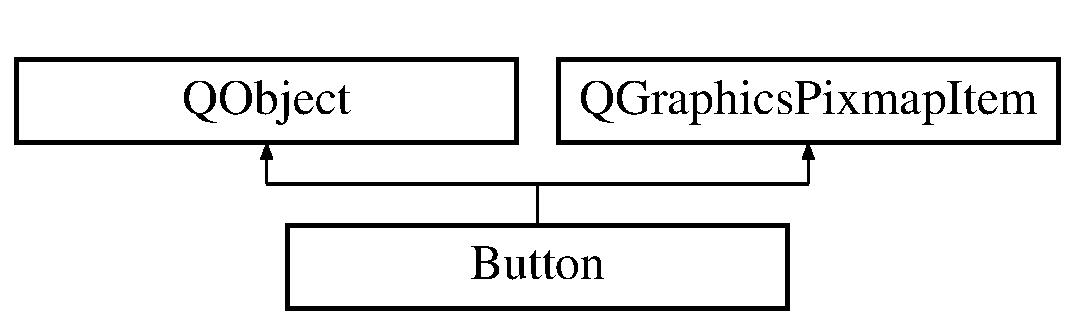
\includegraphics[height=2.000000cm]{classButton}
\end{center}
\end{figure}
\subsection*{Signals}
\begin{DoxyCompactItemize}
\item 
\hypertarget{classButton_a9e7ab4152cb1e7e3beb7f2842f32670c}{void \hyperlink{classButton_a9e7ab4152cb1e7e3beb7f2842f32670c}{clicked} ()}\label{classButton_a9e7ab4152cb1e7e3beb7f2842f32670c}

\begin{DoxyCompactList}\small\item\em Signal to notify if button is clicked. \end{DoxyCompactList}\end{DoxyCompactItemize}
\subsection*{Public Member Functions}
\begin{DoxyCompactItemize}
\item 
\hyperlink{classButton_abbf00c9df181d84d36e915ef712e024c}{Button} (const char $\ast$idle\-\_\-image\-\_\-path, const char $\ast$hover\-\_\-image\-\_\-path, int screen\-\_\-height, int screen\-\_\-width)
\begin{DoxyCompactList}\small\item\em The Constructor for button class. \end{DoxyCompactList}\item 
void \hyperlink{classButton_a17d8eb0c904605b223bbc00c75655315}{mouse\-Press\-Event} (Q\-Graphics\-Scene\-Mouse\-Event $\ast$event)
\begin{DoxyCompactList}\small\item\em Function called when button gets clicked. \end{DoxyCompactList}\item 
void \hyperlink{classButton_a633a9684818bc5d300a622a00064f09c}{hover\-Enter\-Event} (Q\-Graphics\-Scene\-Hover\-Event $\ast$event)
\begin{DoxyCompactList}\small\item\em Function called when mouse cursor touches the button. \end{DoxyCompactList}\item 
void \hyperlink{classButton_a1689a97690d9469ce8350d24db0d7485}{hover\-Leave\-Event} (Q\-Graphics\-Scene\-Hover\-Event $\ast$event)
\begin{DoxyCompactList}\small\item\em Function called when mouse cursor leaves the button. \end{DoxyCompactList}\end{DoxyCompactItemize}


\subsection{Detailed Description}
All the buttons displayed in Main Menu. 

\subsection{Constructor \& Destructor Documentation}
\hypertarget{classButton_abbf00c9df181d84d36e915ef712e024c}{\index{Button@{Button}!Button@{Button}}
\index{Button@{Button}!Button@{Button}}
\subsubsection[{Button}]{\setlength{\rightskip}{0pt plus 5cm}Button\-::\-Button (
\begin{DoxyParamCaption}
\item[{const char $\ast$}]{idle\-\_\-image\-\_\-path, }
\item[{const char $\ast$}]{hover\-\_\-image\-\_\-path, }
\item[{int}]{screen\-\_\-height, }
\item[{int}]{screen\-\_\-width}
\end{DoxyParamCaption}
)}}\label{classButton_abbf00c9df181d84d36e915ef712e024c}


The Constructor for button class. 


\begin{DoxyParams}{Parameters}
{\em idle\-\_\-image\-\_\-path} & file path containing image for idle\-Pix\-Map \\
\hline
{\em hover\-\_\-image\-\_\-path} & file path containing image for hover\-Pix\-Map \\
\hline
{\em screen\-\_\-height} & Height of the Screen \\
\hline
{\em screen\-\_\-width} & Width of the Screen \\
\hline
\end{DoxyParams}


\subsection{Member Function Documentation}
\hypertarget{classButton_a633a9684818bc5d300a622a00064f09c}{\index{Button@{Button}!hover\-Enter\-Event@{hover\-Enter\-Event}}
\index{hover\-Enter\-Event@{hover\-Enter\-Event}!Button@{Button}}
\subsubsection[{hover\-Enter\-Event}]{\setlength{\rightskip}{0pt plus 5cm}void Button\-::hover\-Enter\-Event (
\begin{DoxyParamCaption}
\item[{Q\-Graphics\-Scene\-Hover\-Event $\ast$}]{event}
\end{DoxyParamCaption}
)}}\label{classButton_a633a9684818bc5d300a622a00064f09c}


Function called when mouse cursor touches the button. 


\begin{DoxyParams}{Parameters}
{\em event} & The Event received \\
\hline
\end{DoxyParams}
\hypertarget{classButton_a1689a97690d9469ce8350d24db0d7485}{\index{Button@{Button}!hover\-Leave\-Event@{hover\-Leave\-Event}}
\index{hover\-Leave\-Event@{hover\-Leave\-Event}!Button@{Button}}
\subsubsection[{hover\-Leave\-Event}]{\setlength{\rightskip}{0pt plus 5cm}void Button\-::hover\-Leave\-Event (
\begin{DoxyParamCaption}
\item[{Q\-Graphics\-Scene\-Hover\-Event $\ast$}]{event}
\end{DoxyParamCaption}
)}}\label{classButton_a1689a97690d9469ce8350d24db0d7485}


Function called when mouse cursor leaves the button. 


\begin{DoxyParams}{Parameters}
{\em event} & The Event received \\
\hline
\end{DoxyParams}
\hypertarget{classButton_a17d8eb0c904605b223bbc00c75655315}{\index{Button@{Button}!mouse\-Press\-Event@{mouse\-Press\-Event}}
\index{mouse\-Press\-Event@{mouse\-Press\-Event}!Button@{Button}}
\subsubsection[{mouse\-Press\-Event}]{\setlength{\rightskip}{0pt plus 5cm}void Button\-::mouse\-Press\-Event (
\begin{DoxyParamCaption}
\item[{Q\-Graphics\-Scene\-Mouse\-Event $\ast$}]{event}
\end{DoxyParamCaption}
)}}\label{classButton_a17d8eb0c904605b223bbc00c75655315}


Function called when button gets clicked. 


\begin{DoxyParams}{Parameters}
{\em event} & The Event received \\
\hline
\end{DoxyParams}


The documentation for this class was generated from the following file\-:\begin{DoxyCompactItemize}
\item 
button.\-h\end{DoxyCompactItemize}

\hypertarget{classChoiceServerClientStart}{\section{Choice\-Server\-Client\-Start Class Reference}
\label{classChoiceServerClientStart}\index{Choice\-Server\-Client\-Start@{Choice\-Server\-Client\-Start}}
}


The Choice between \hyperlink{classServer}{Server} Client\-Start class.  




{\ttfamily \#include $<$choiceserverclientstart.\-h$>$}

Inheritance diagram for Choice\-Server\-Client\-Start\-:\begin{figure}[H]
\begin{center}
\leavevmode
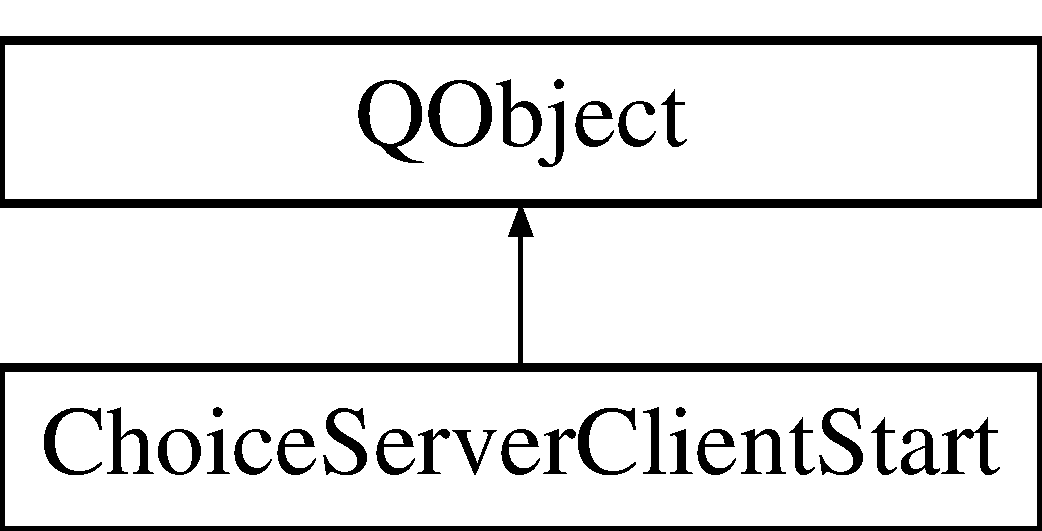
\includegraphics[height=2.000000cm]{classChoiceServerClientStart}
\end{center}
\end{figure}
\subsection*{Public Member Functions}
\begin{DoxyCompactItemize}
\item 
\hyperlink{classChoiceServerClientStart_aed01cdd365bf5bdd25d124e9cf53b4c2}{Choice\-Server\-Client\-Start} (Q\-Graphics\-Scene $\ast$, \hyperlink{classInputHandler}{Input\-Handler} $\ast$, const char $\ast$, int, int, int, \hyperlink{classClient}{Client} $\ast$, \hyperlink{classServer}{Server} $\ast$, Q\-Label $\ast$, Q\-Widget $\ast$parent=N\-U\-L\-L)
\begin{DoxyCompactList}\small\item\em Constructor. \end{DoxyCompactList}\item 
\hypertarget{classChoiceServerClientStart_a26594a0283a1d48b839d8d7bcd578b91}{\hyperlink{classChoiceServerClientStart_a26594a0283a1d48b839d8d7bcd578b91}{$\sim$\-Choice\-Server\-Client\-Start} ()}\label{classChoiceServerClientStart_a26594a0283a1d48b839d8d7bcd578b91}

\begin{DoxyCompactList}\small\item\em Destructor. \end{DoxyCompactList}\item 
\hypertarget{classChoiceServerClientStart_ad23b654ec5ad197c27f45514d57cb8bf}{void \hyperlink{classChoiceServerClientStart_ad23b654ec5ad197c27f45514d57cb8bf}{display\-Start\-Menu} ()}\label{classChoiceServerClientStart_ad23b654ec5ad197c27f45514d57cb8bf}

\begin{DoxyCompactList}\small\item\em Display Start Menu. \end{DoxyCompactList}\end{DoxyCompactItemize}


\subsection{Detailed Description}
The Choice between \hyperlink{classServer}{Server} Client\-Start class. 

\subsection{Constructor \& Destructor Documentation}
\hypertarget{classChoiceServerClientStart_aed01cdd365bf5bdd25d124e9cf53b4c2}{\index{Choice\-Server\-Client\-Start@{Choice\-Server\-Client\-Start}!Choice\-Server\-Client\-Start@{Choice\-Server\-Client\-Start}}
\index{Choice\-Server\-Client\-Start@{Choice\-Server\-Client\-Start}!ChoiceServerClientStart@{Choice\-Server\-Client\-Start}}
\subsubsection[{Choice\-Server\-Client\-Start}]{\setlength{\rightskip}{0pt plus 5cm}Choice\-Server\-Client\-Start\-::\-Choice\-Server\-Client\-Start (
\begin{DoxyParamCaption}
\item[{Q\-Graphics\-Scene $\ast$}]{, }
\item[{{\bf Input\-Handler} $\ast$}]{, }
\item[{const char $\ast$}]{, }
\item[{int}]{, }
\item[{int}]{, }
\item[{int}]{, }
\item[{{\bf Client} $\ast$}]{, }
\item[{{\bf Server} $\ast$}]{, }
\item[{Q\-Label $\ast$}]{, }
\item[{Q\-Widget $\ast$}]{parent = {\ttfamily NULL}}
\end{DoxyParamCaption}
)}}\label{classChoiceServerClientStart_aed01cdd365bf5bdd25d124e9cf53b4c2}


Constructor. 


\begin{DoxyParams}{Parameters}
{\em parent} & \\
\hline
\end{DoxyParams}


The documentation for this class was generated from the following file\-:\begin{DoxyCompactItemize}
\item 
choiceserverclientstart.\-h\end{DoxyCompactItemize}

\hypertarget{classClient}{\section{Client Class Reference}
\label{classClient}\index{Client@{Client}}
}


The Class to Create a \hyperlink{classClient}{Client}.  




{\ttfamily \#include $<$client.\-h$>$}

Inheritance diagram for Client\-:\begin{figure}[H]
\begin{center}
\leavevmode
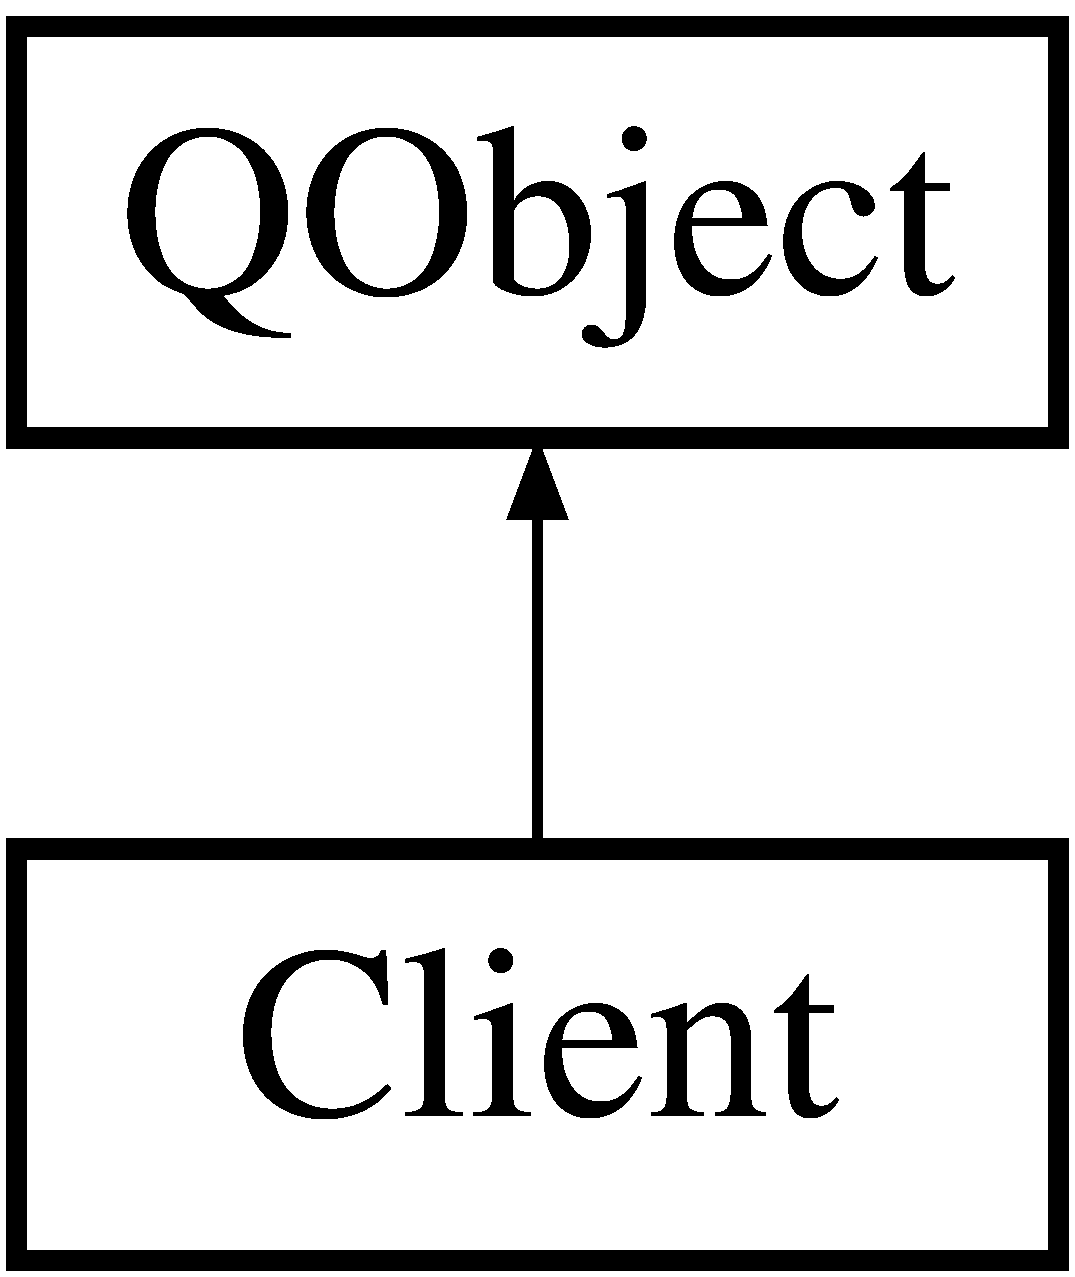
\includegraphics[height=2.000000cm]{classClient}
\end{center}
\end{figure}
\subsection*{Signals}
\begin{DoxyCompactItemize}
\item 
\hypertarget{classClient_ab1fad07406e7086043ac689a03005480}{void \hyperlink{classClient_ab1fad07406e7086043ac689a03005480}{closed} ()}\label{classClient_ab1fad07406e7086043ac689a03005480}

\begin{DoxyCompactList}\small\item\em Signal to be sent when \hyperlink{classClient}{Client} closes. \end{DoxyCompactList}\item 
\hypertarget{classClient_ad6da73c1bc1ff62071e24825a4254433}{void \hyperlink{classClient_ad6da73c1bc1ff62071e24825a4254433}{text\-Changed} (Q\-String)}\label{classClient_ad6da73c1bc1ff62071e24825a4254433}

\begin{DoxyCompactList}\small\item\em Text Change Function. \end{DoxyCompactList}\end{DoxyCompactItemize}
\subsection*{Public Member Functions}
\begin{DoxyCompactItemize}
\item 
\hyperlink{classClient_a78171ef219443f177e1b7d80d0798d55}{Client} (Q\-Application $\ast$, int, Q\-Graphics\-Scene $\ast$, \hyperlink{classInputHandler}{Input\-Handler} $\ast$, int, int, Q\-Label $\ast$, Q\-Object $\ast$parent=0)
\begin{DoxyCompactList}\small\item\em \hyperlink{classClient}{Client} Constructor. \end{DoxyCompactList}\item 
\hypertarget{classClient_a840e519ca781888cbd54181572ebe3a7}{\hyperlink{classClient_a840e519ca781888cbd54181572ebe3a7}{$\sim$\-Client} ()}\label{classClient_a840e519ca781888cbd54181572ebe3a7}

\begin{DoxyCompactList}\small\item\em \hyperlink{classClient}{Client} Destructor. \end{DoxyCompactList}\item 
int \hyperlink{classClient_ad8fcb654942cf5d804010be882164d67}{get\-Array\-Index} ()
\begin{DoxyCompactList}\small\item\em Get the Player I\-D. \end{DoxyCompactList}\item 
Q\-Web\-Socket $\ast$ \hyperlink{classClient_a865e84b80885b731dfee9752e98485a8}{get\-Client\-Web\-Socket} ()
\begin{DoxyCompactList}\small\item\em The \hyperlink{classClient}{Client} Websocket. \end{DoxyCompactList}\item 
\hypertarget{classClient_a1b60e473f218c0910448adbef2cf644b}{void \hyperlink{classClient_a1b60e473f218c0910448adbef2cf644b}{Display\-Score} (Q\-String)}\label{classClient_a1b60e473f218c0910448adbef2cf644b}

\begin{DoxyCompactList}\small\item\em Display The Score. \end{DoxyCompactList}\item 
\hypertarget{classClient_af015d89a945001f35a8e8c3bb0459d4a}{void \hyperlink{classClient_af015d89a945001f35a8e8c3bb0459d4a}{connect\-To\-Server} (Q\-Url, Q\-Graphics\-Text\-Item $\ast$, Q\-String)}\label{classClient_af015d89a945001f35a8e8c3bb0459d4a}

\begin{DoxyCompactList}\small\item\em Connect To \hyperlink{classServer}{Server}. \end{DoxyCompactList}\end{DoxyCompactItemize}
\subsection*{Public Attributes}
\begin{DoxyCompactItemize}
\item 
\hypertarget{classClient_afd59ea5b74c1b9d4529cc7f911808e05}{\hyperlink{classGameState}{Game\-State} $\ast$ \hyperlink{classClient_afd59ea5b74c1b9d4529cc7f911808e05}{game\-Pointer}}\label{classClient_afd59ea5b74c1b9d4529cc7f911808e05}

\begin{DoxyCompactList}\small\item\em The \hyperlink{classGameState}{Game\-State} Pointer. \end{DoxyCompactList}\end{DoxyCompactItemize}


\subsection{Detailed Description}
The Class to Create a \hyperlink{classClient}{Client}. 

\subsection{Constructor \& Destructor Documentation}
\hypertarget{classClient_a78171ef219443f177e1b7d80d0798d55}{\index{Client@{Client}!Client@{Client}}
\index{Client@{Client}!Client@{Client}}
\subsubsection[{Client}]{\setlength{\rightskip}{0pt plus 5cm}Client\-::\-Client (
\begin{DoxyParamCaption}
\item[{Q\-Application $\ast$}]{, }
\item[{int}]{, }
\item[{Q\-Graphics\-Scene $\ast$}]{, }
\item[{{\bf Input\-Handler} $\ast$}]{, }
\item[{int}]{, }
\item[{int}]{, }
\item[{Q\-Label $\ast$}]{, }
\item[{Q\-Object $\ast$}]{parent = {\ttfamily 0}}
\end{DoxyParamCaption}
)}}\label{classClient_a78171ef219443f177e1b7d80d0798d55}


\hyperlink{classClient}{Client} Constructor. 


\begin{DoxyParams}{Parameters}
{\em parent} & \\
\hline
\end{DoxyParams}


\subsection{Member Function Documentation}
\hypertarget{classClient_ad8fcb654942cf5d804010be882164d67}{\index{Client@{Client}!get\-Array\-Index@{get\-Array\-Index}}
\index{get\-Array\-Index@{get\-Array\-Index}!Client@{Client}}
\subsubsection[{get\-Array\-Index}]{\setlength{\rightskip}{0pt plus 5cm}int Client\-::get\-Array\-Index (
\begin{DoxyParamCaption}
{}
\end{DoxyParamCaption}
)}}\label{classClient_ad8fcb654942cf5d804010be882164d67}


Get the Player I\-D. 

\begin{DoxyReturn}{Returns}
Player I\-D 
\end{DoxyReturn}
\hypertarget{classClient_a865e84b80885b731dfee9752e98485a8}{\index{Client@{Client}!get\-Client\-Web\-Socket@{get\-Client\-Web\-Socket}}
\index{get\-Client\-Web\-Socket@{get\-Client\-Web\-Socket}!Client@{Client}}
\subsubsection[{get\-Client\-Web\-Socket}]{\setlength{\rightskip}{0pt plus 5cm}Q\-Web\-Socket$\ast$ Client\-::get\-Client\-Web\-Socket (
\begin{DoxyParamCaption}
{}
\end{DoxyParamCaption}
)}}\label{classClient_a865e84b80885b731dfee9752e98485a8}


The \hyperlink{classClient}{Client} Websocket. 

\begin{DoxyReturn}{Returns}
clientwebsocket 
\end{DoxyReturn}


The documentation for this class was generated from the following file\-:\begin{DoxyCompactItemize}
\item 
client.\-h\end{DoxyCompactItemize}

\hypertarget{classComputerInputComponent}{\section{Computer\-Input\-Component Class Reference}
\label{classComputerInputComponent}\index{Computer\-Input\-Component@{Computer\-Input\-Component}}
}


The input component to handle state changes for non human input.  




{\ttfamily \#include $<$computerinputcomponent.\-h$>$}

Inheritance diagram for Computer\-Input\-Component\-:\begin{figure}[H]
\begin{center}
\leavevmode
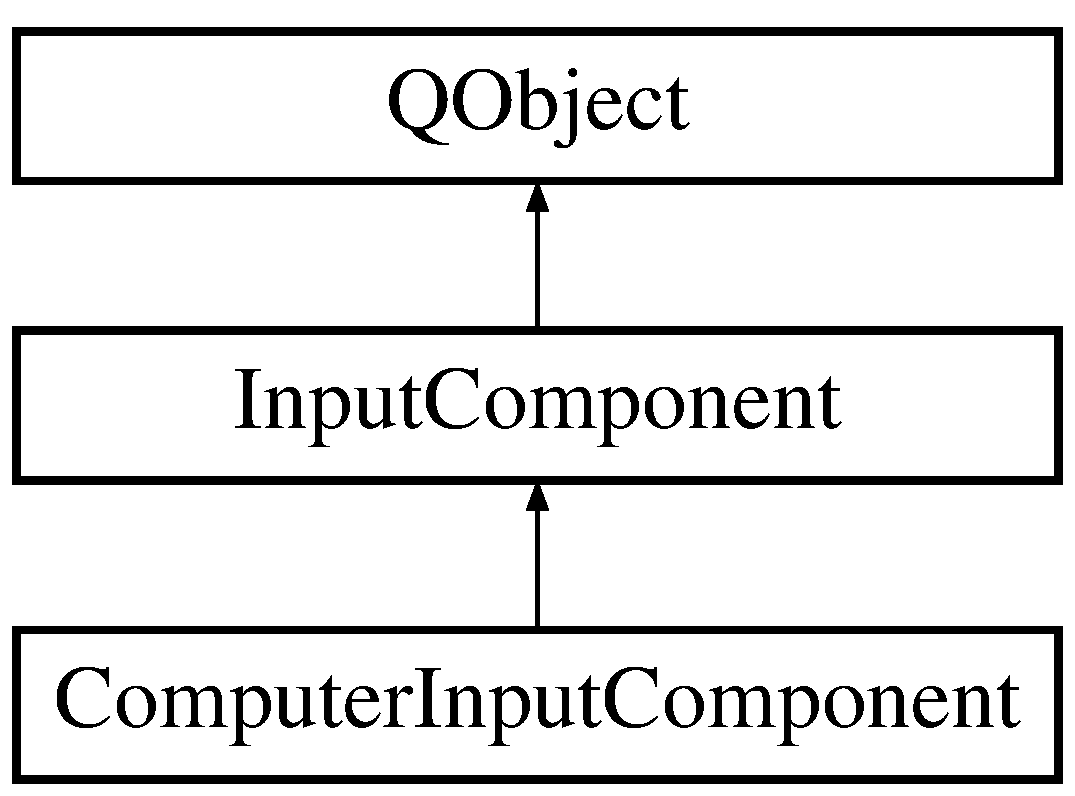
\includegraphics[height=3.000000cm]{classComputerInputComponent}
\end{center}
\end{figure}
\subsection*{Public Member Functions}
\begin{DoxyCompactItemize}
\item 
\hypertarget{classComputerInputComponent_a9fe5c3b8e0c08f505856828d45d941b2}{\hyperlink{classComputerInputComponent_a9fe5c3b8e0c08f505856828d45d941b2}{Computer\-Input\-Component} ()}\label{classComputerInputComponent_a9fe5c3b8e0c08f505856828d45d941b2}

\begin{DoxyCompactList}\small\item\em Constructor. \end{DoxyCompactList}\item 
\hypertarget{classComputerInputComponent_a58e35dc2bcec2ee35fdca85b25f9dbf0}{virtual \hyperlink{classComputerInputComponent_a58e35dc2bcec2ee35fdca85b25f9dbf0}{$\sim$\-Computer\-Input\-Component} ()}\label{classComputerInputComponent_a58e35dc2bcec2ee35fdca85b25f9dbf0}

\begin{DoxyCompactList}\small\item\em Destructor. \end{DoxyCompactList}\item 
virtual void \hyperlink{classComputerInputComponent_abddd2bdc7efb465f49173a3634148bbc}{update} (\hyperlink{classGameObject}{Game\-Object} \&game\-Object)
\begin{DoxyCompactList}\small\item\em Updates the state of the corresponding \hyperlink{classGameObject}{Game\-Object}. \end{DoxyCompactList}\item 
virtual bool \hyperlink{classComputerInputComponent_a20fda9adf00a1be24b9bcca0b8662a35}{accepts\-Input} ()
\begin{DoxyCompactList}\small\item\em Checks whether the \hyperlink{classGameObject}{Game\-Object} accepts input. \end{DoxyCompactList}\end{DoxyCompactItemize}
\subsection*{Additional Inherited Members}


\subsection{Detailed Description}
The input component to handle state changes for non human input. 

This is handles state changes for all the monsters and updates them as needed 

\subsection{Member Function Documentation}
\hypertarget{classComputerInputComponent_a20fda9adf00a1be24b9bcca0b8662a35}{\index{Computer\-Input\-Component@{Computer\-Input\-Component}!accepts\-Input@{accepts\-Input}}
\index{accepts\-Input@{accepts\-Input}!ComputerInputComponent@{Computer\-Input\-Component}}
\subsubsection[{accepts\-Input}]{\setlength{\rightskip}{0pt plus 5cm}virtual bool Computer\-Input\-Component\-::accepts\-Input (
\begin{DoxyParamCaption}
{}
\end{DoxyParamCaption}
)\hspace{0.3cm}{\ttfamily [virtual]}}}\label{classComputerInputComponent_a20fda9adf00a1be24b9bcca0b8662a35}


Checks whether the \hyperlink{classGameObject}{Game\-Object} accepts input. 

\begin{DoxyReturn}{Returns}
false, as \hyperlink{classGameObject}{Game\-Object} with \hyperlink{classComputerInputComponent}{Computer\-Input\-Component} does not accept input 
\end{DoxyReturn}


Implements \hyperlink{classInputComponent_a27a4de99780ddf7d7a4f9d469f13640c}{Input\-Component}.

\hypertarget{classComputerInputComponent_abddd2bdc7efb465f49173a3634148bbc}{\index{Computer\-Input\-Component@{Computer\-Input\-Component}!update@{update}}
\index{update@{update}!ComputerInputComponent@{Computer\-Input\-Component}}
\subsubsection[{update}]{\setlength{\rightskip}{0pt plus 5cm}virtual void Computer\-Input\-Component\-::update (
\begin{DoxyParamCaption}
\item[{{\bf Game\-Object} \&}]{game\-Object}
\end{DoxyParamCaption}
)\hspace{0.3cm}{\ttfamily [virtual]}}}\label{classComputerInputComponent_abddd2bdc7efb465f49173a3634148bbc}


Updates the state of the corresponding \hyperlink{classGameObject}{Game\-Object}. 


\begin{DoxyParams}{Parameters}
{\em game\-Object} & the \hyperlink{classGameObject}{Game\-Object} whose state will be updated \\
\hline
\end{DoxyParams}


Implements \hyperlink{classInputComponent_a93e790f7279e842ee249fefe7dbf7b32}{Input\-Component}.



The documentation for this class was generated from the following file\-:\begin{DoxyCompactItemize}
\item 
computerinputcomponent.\-h\end{DoxyCompactItemize}

\hypertarget{classDeadLeft}{\section{Dead\-Left Class Reference}
\label{classDeadLeft}\index{Dead\-Left@{Dead\-Left}}
}


The state in which the player is dead facing left This also handles the responds to key press and key release inputs so as to change the state of the \hyperlink{classGameObject}{Game\-Object}.  




{\ttfamily \#include $<$deadleft.\-h$>$}

Inheritance diagram for Dead\-Left\-:\begin{figure}[H]
\begin{center}
\leavevmode
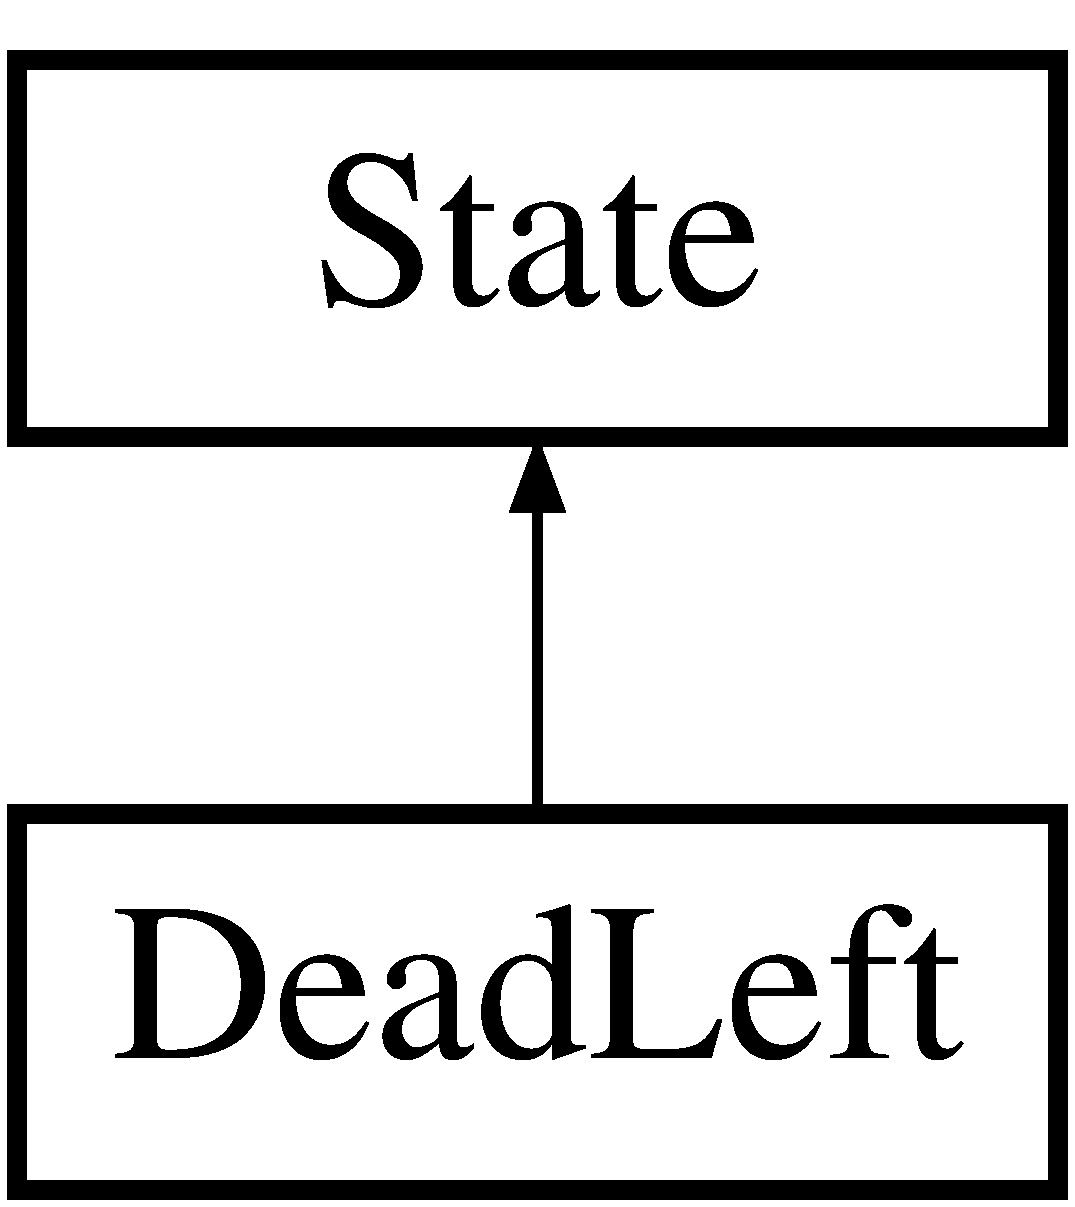
\includegraphics[height=2.000000cm]{classDeadLeft}
\end{center}
\end{figure}
\subsection*{Public Member Functions}
\begin{DoxyCompactItemize}
\item 
\hypertarget{classDeadLeft_ad1149774bf2977166a9ceffa51c45c17}{\hyperlink{classDeadLeft_ad1149774bf2977166a9ceffa51c45c17}{Dead\-Left} ()}\label{classDeadLeft_ad1149774bf2977166a9ceffa51c45c17}

\begin{DoxyCompactList}\small\item\em Constructor. \end{DoxyCompactList}\item 
\hypertarget{classDeadLeft_a8706b3c84e6916d3c863c47c7fa51584}{\hyperlink{classDeadLeft_a8706b3c84e6916d3c863c47c7fa51584}{$\sim$\-Dead\-Left} ()}\label{classDeadLeft_a8706b3c84e6916d3c863c47c7fa51584}

\begin{DoxyCompactList}\small\item\em Destructor. \end{DoxyCompactList}\item 
\hyperlink{classState}{State} $\ast$ \hyperlink{classDeadLeft_a641116efda392a1c6437e9034443a1ea}{update} (\hyperlink{classInputComponent}{Input\-Component} $\ast$input\-Component, std\-::set$<$ Qt\-::\-Key $>$ key)
\begin{DoxyCompactList}\small\item\em Updates the state on the basis of the keys currently pressed. \end{DoxyCompactList}\item 
\hyperlink{namespaceenumerator_a5fc7b342c2c633e1037b07cea237a222}{enumerator\-::\-State} \hyperlink{classDeadLeft_a564f47ceebef43f5553072c446b3c12f}{type} ()
\begin{DoxyCompactList}\small\item\em Provides the type of the \hyperlink{classState}{State}, i.\-e., \hyperlink{classDeadLeft}{Dead\-Left}. \end{DoxyCompactList}\end{DoxyCompactItemize}


\subsection{Detailed Description}
The state in which the player is dead facing left This also handles the responds to key press and key release inputs so as to change the state of the \hyperlink{classGameObject}{Game\-Object}. 

\subsection{Member Function Documentation}
\hypertarget{classDeadLeft_a564f47ceebef43f5553072c446b3c12f}{\index{Dead\-Left@{Dead\-Left}!type@{type}}
\index{type@{type}!DeadLeft@{Dead\-Left}}
\subsubsection[{type}]{\setlength{\rightskip}{0pt plus 5cm}{\bf enumerator\-::\-State} Dead\-Left\-::type (
\begin{DoxyParamCaption}
{}
\end{DoxyParamCaption}
)\hspace{0.3cm}{\ttfamily [virtual]}}}\label{classDeadLeft_a564f47ceebef43f5553072c446b3c12f}


Provides the type of the \hyperlink{classState}{State}, i.\-e., \hyperlink{classDeadLeft}{Dead\-Left}. 

\begin{DoxyReturn}{Returns}
enumerator\-::\-State\-::\-D\-E\-A\-D\-\_\-\-L\-E\-F\-T 
\end{DoxyReturn}


Implements \hyperlink{classState_a8c6cc1ff1ecdf88e586f857339b7e071}{State}.

\hypertarget{classDeadLeft_a641116efda392a1c6437e9034443a1ea}{\index{Dead\-Left@{Dead\-Left}!update@{update}}
\index{update@{update}!DeadLeft@{Dead\-Left}}
\subsubsection[{update}]{\setlength{\rightskip}{0pt plus 5cm}{\bf State}$\ast$ Dead\-Left\-::update (
\begin{DoxyParamCaption}
\item[{{\bf Input\-Component} $\ast$}]{input\-Component, }
\item[{std\-::set$<$ Qt\-::\-Key $>$}]{key}
\end{DoxyParamCaption}
)\hspace{0.3cm}{\ttfamily [virtual]}}}\label{classDeadLeft_a641116efda392a1c6437e9034443a1ea}


Updates the state on the basis of the keys currently pressed. 


\begin{DoxyParams}{Parameters}
{\em input\-Component} & the \hyperlink{classInputComponent}{Input\-Component} of the \hyperlink{classGameObject}{Game\-Object} whose state is being updated \\
\hline
{\em key} & the set of keys currently pressed \\
\hline
\end{DoxyParams}
\begin{DoxyReturn}{Returns}
the new state 
\end{DoxyReturn}


Implements \hyperlink{classState_a5f2bc9804614c5ca9e7feb7d8c57668d}{State}.



The documentation for this class was generated from the following file\-:\begin{DoxyCompactItemize}
\item 
deadleft.\-h\end{DoxyCompactItemize}

\hypertarget{classDeadRight}{\section{Dead\-Right Class Reference}
\label{classDeadRight}\index{Dead\-Right@{Dead\-Right}}
}


The state in which the player is dead facing right This also handles the responds to key press and key release inputs so as to change the state of the \hyperlink{classGameObject}{Game\-Object}.  




{\ttfamily \#include $<$deadright.\-h$>$}

Inheritance diagram for Dead\-Right\-:\begin{figure}[H]
\begin{center}
\leavevmode
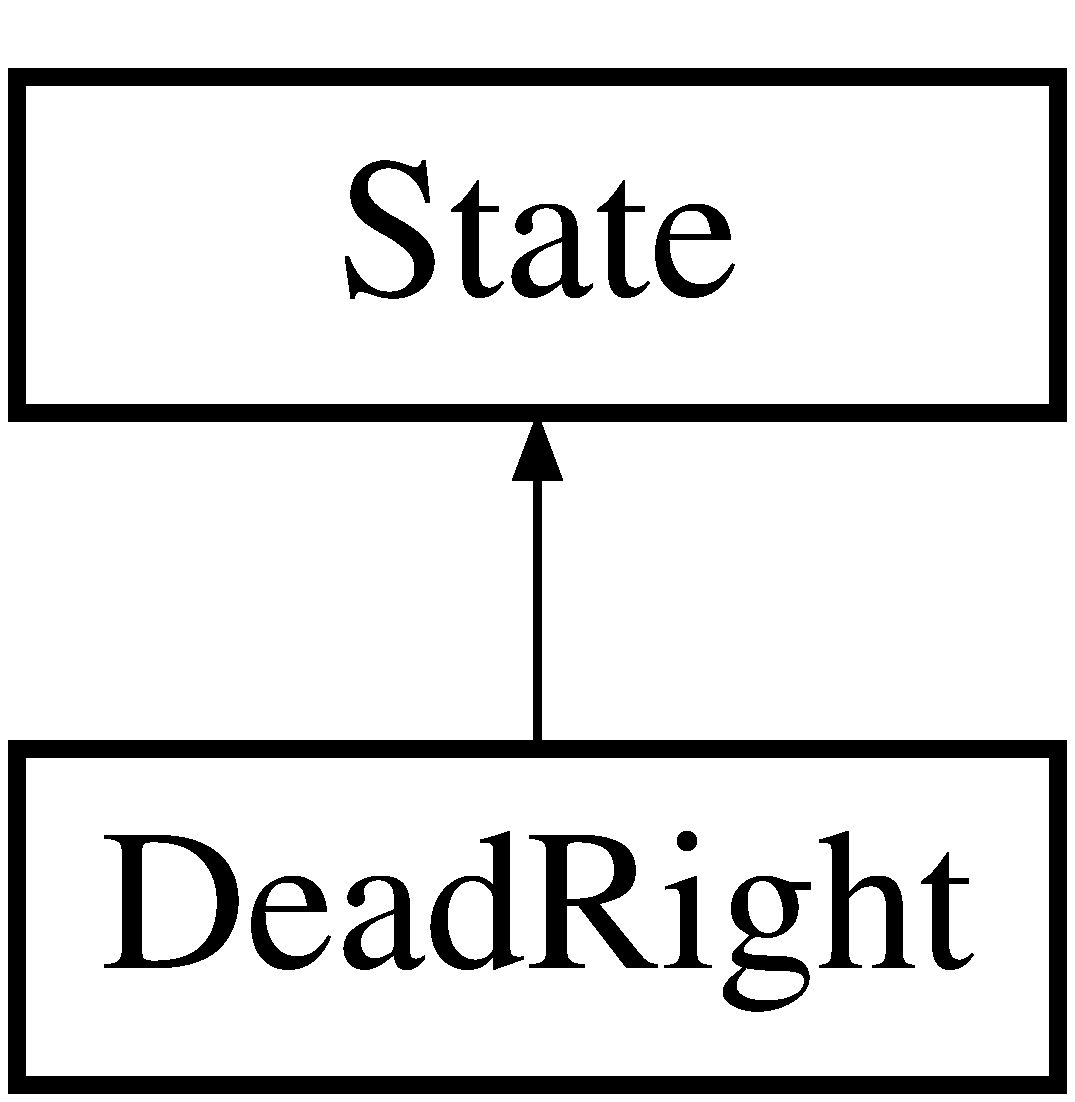
\includegraphics[height=2.000000cm]{classDeadRight}
\end{center}
\end{figure}
\subsection*{Public Member Functions}
\begin{DoxyCompactItemize}
\item 
\hypertarget{classDeadRight_a08aa0bda5faa79706498c10bf7f7ab57}{\hyperlink{classDeadRight_a08aa0bda5faa79706498c10bf7f7ab57}{Dead\-Right} ()}\label{classDeadRight_a08aa0bda5faa79706498c10bf7f7ab57}

\begin{DoxyCompactList}\small\item\em Constructor. \end{DoxyCompactList}\item 
\hypertarget{classDeadRight_a04979ad62939563bb7e995f967536b87}{\hyperlink{classDeadRight_a04979ad62939563bb7e995f967536b87}{$\sim$\-Dead\-Right} ()}\label{classDeadRight_a04979ad62939563bb7e995f967536b87}

\begin{DoxyCompactList}\small\item\em Destructor. \end{DoxyCompactList}\item 
\hyperlink{classState}{State} $\ast$ \hyperlink{classDeadRight_a90bbfab63b08a87dd2b36bbdb8830aa5}{update} (\hyperlink{classInputComponent}{Input\-Component} $\ast$, std\-::set$<$ Qt\-::\-Key $>$)
\begin{DoxyCompactList}\small\item\em Updates the state on the basis of the keys currently pressed. \end{DoxyCompactList}\item 
\hyperlink{namespaceenumerator_a5fc7b342c2c633e1037b07cea237a222}{enumerator\-::\-State} \hyperlink{classDeadRight_abd8e52205ddafd19858a81f25cd87106}{type} ()
\begin{DoxyCompactList}\small\item\em Provides the type of the \hyperlink{classState}{State}, i.\-e., \hyperlink{classDeadLeft}{Dead\-Left}. \end{DoxyCompactList}\end{DoxyCompactItemize}


\subsection{Detailed Description}
The state in which the player is dead facing right This also handles the responds to key press and key release inputs so as to change the state of the \hyperlink{classGameObject}{Game\-Object}. 

\subsection{Member Function Documentation}
\hypertarget{classDeadRight_abd8e52205ddafd19858a81f25cd87106}{\index{Dead\-Right@{Dead\-Right}!type@{type}}
\index{type@{type}!DeadRight@{Dead\-Right}}
\subsubsection[{type}]{\setlength{\rightskip}{0pt plus 5cm}{\bf enumerator\-::\-State} Dead\-Right\-::type (
\begin{DoxyParamCaption}
{}
\end{DoxyParamCaption}
)\hspace{0.3cm}{\ttfamily [virtual]}}}\label{classDeadRight_abd8e52205ddafd19858a81f25cd87106}


Provides the type of the \hyperlink{classState}{State}, i.\-e., \hyperlink{classDeadLeft}{Dead\-Left}. 

\begin{DoxyReturn}{Returns}
enumerator\-::\-State\-::\-D\-E\-A\-D\-\_\-\-L\-E\-F\-T 
\end{DoxyReturn}


Implements \hyperlink{classState_a8c6cc1ff1ecdf88e586f857339b7e071}{State}.

\hypertarget{classDeadRight_a90bbfab63b08a87dd2b36bbdb8830aa5}{\index{Dead\-Right@{Dead\-Right}!update@{update}}
\index{update@{update}!DeadRight@{Dead\-Right}}
\subsubsection[{update}]{\setlength{\rightskip}{0pt plus 5cm}{\bf State}$\ast$ Dead\-Right\-::update (
\begin{DoxyParamCaption}
\item[{{\bf Input\-Component} $\ast$}]{, }
\item[{std\-::set$<$ Qt\-::\-Key $>$}]{}
\end{DoxyParamCaption}
)\hspace{0.3cm}{\ttfamily [virtual]}}}\label{classDeadRight_a90bbfab63b08a87dd2b36bbdb8830aa5}


Updates the state on the basis of the keys currently pressed. 


\begin{DoxyParams}{Parameters}
{\em input\-Component} & the \hyperlink{classInputComponent}{Input\-Component} of the \hyperlink{classGameObject}{Game\-Object} whose state is being updated \\
\hline
{\em key} & the set of keys currently pressed \\
\hline
\end{DoxyParams}
\begin{DoxyReturn}{Returns}
the new state 
\end{DoxyReturn}


Implements \hyperlink{classState_a5f2bc9804614c5ca9e7feb7d8c57668d}{State}.



The documentation for this class was generated from the following file\-:\begin{DoxyCompactItemize}
\item 
deadright.\-h\end{DoxyCompactItemize}

\hypertarget{classDiamond}{\section{Diamond Class Reference}
\label{classDiamond}\index{Diamond@{Diamond}}
}


Describes a \hyperlink{classDiamond}{Diamond} Handles the drawing, placement on screen, and position of a diamond.  




{\ttfamily \#include $<$diamond.\-h$>$}

Inheritance diagram for Diamond\-:\begin{figure}[H]
\begin{center}
\leavevmode
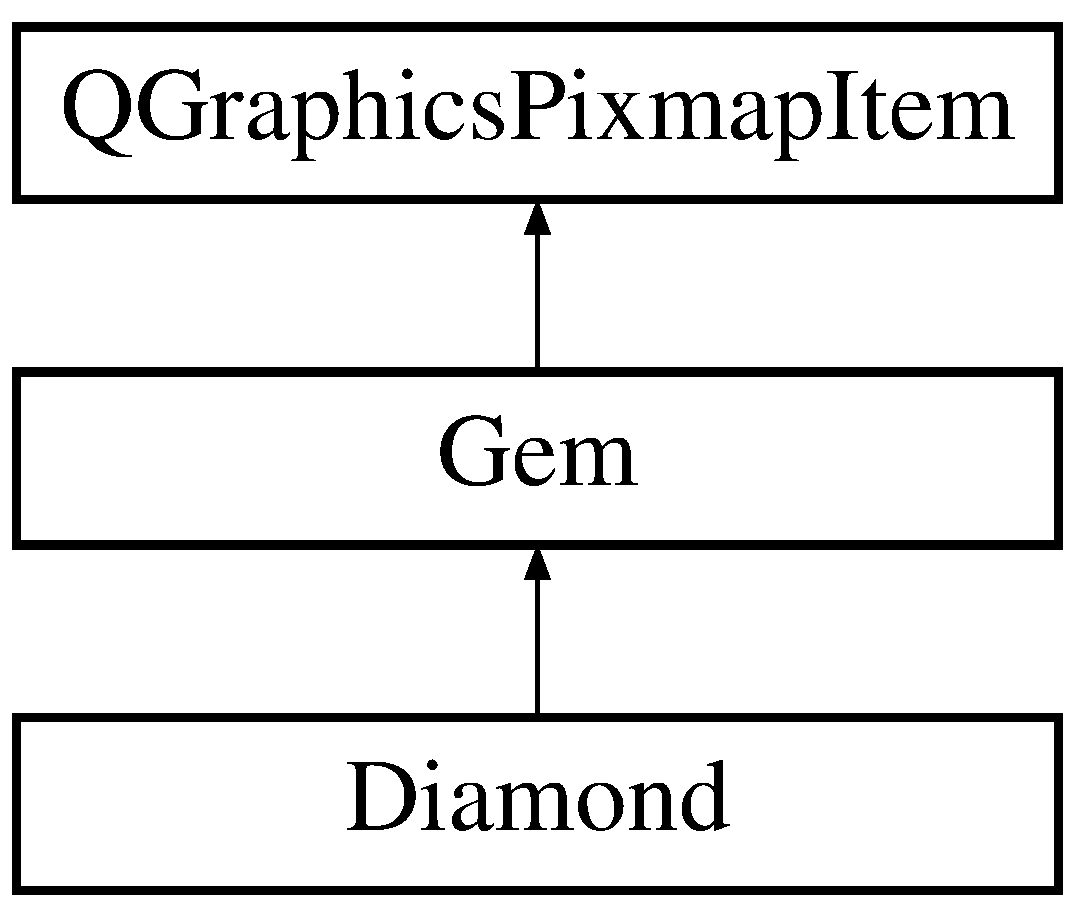
\includegraphics[height=3.000000cm]{classDiamond}
\end{center}
\end{figure}
\subsection*{Public Member Functions}
\begin{DoxyCompactItemize}
\item 
\hyperlink{classDiamond_af9b451f4382e3cbfba2bc34969e1ac3a}{Diamond} (std\-::string image\-\_\-location, int width, int height, qreal x\-\_\-coordinate, qreal y\-\_\-coordinate, int score\-\_\-of\-\_\-gem)
\begin{DoxyCompactList}\small\item\em Create a diamond. \end{DoxyCompactList}\item 
void \hyperlink{classDiamond_a7139292b0be9a93f99f48e6c00fac072}{draw\-Gem} (Q\-Graphics\-Scene $\ast$scene)
\begin{DoxyCompactList}\small\item\em Draws the diamond to the scene. \end{DoxyCompactList}\end{DoxyCompactItemize}


\subsection{Detailed Description}
Describes a \hyperlink{classDiamond}{Diamond} Handles the drawing, placement on screen, and position of a diamond. 

\subsection{Constructor \& Destructor Documentation}
\hypertarget{classDiamond_af9b451f4382e3cbfba2bc34969e1ac3a}{\index{Diamond@{Diamond}!Diamond@{Diamond}}
\index{Diamond@{Diamond}!Diamond@{Diamond}}
\subsubsection[{Diamond}]{\setlength{\rightskip}{0pt plus 5cm}Diamond\-::\-Diamond (
\begin{DoxyParamCaption}
\item[{std\-::string}]{image\-\_\-location, }
\item[{int}]{width, }
\item[{int}]{height, }
\item[{qreal}]{x\-\_\-coordinate, }
\item[{qreal}]{y\-\_\-coordinate, }
\item[{int}]{score\-\_\-of\-\_\-gem}
\end{DoxyParamCaption}
)}}\label{classDiamond_af9b451f4382e3cbfba2bc34969e1ac3a}


Create a diamond. 


\begin{DoxyParams}{Parameters}
{\em image\-\_\-location} & the file path of the images to render the diamond \\
\hline
{\em width} & the width of the diamond \\
\hline
{\em height} & the height of the diamond \\
\hline
{\em x\-\_\-coordinate} & the x coordinate on the screen \\
\hline
{\em y\-\_\-coordinate} & the y coordinate on the screen \\
\hline
{\em score\-\_\-of\-\_\-gem} & the score obtained by taking the diamond \\
\hline
\end{DoxyParams}


\subsection{Member Function Documentation}
\hypertarget{classDiamond_a7139292b0be9a93f99f48e6c00fac072}{\index{Diamond@{Diamond}!draw\-Gem@{draw\-Gem}}
\index{draw\-Gem@{draw\-Gem}!Diamond@{Diamond}}
\subsubsection[{draw\-Gem}]{\setlength{\rightskip}{0pt plus 5cm}void Diamond\-::draw\-Gem (
\begin{DoxyParamCaption}
\item[{Q\-Graphics\-Scene $\ast$}]{scene}
\end{DoxyParamCaption}
)\hspace{0.3cm}{\ttfamily [virtual]}}}\label{classDiamond_a7139292b0be9a93f99f48e6c00fac072}


Draws the diamond to the scene. 


\begin{DoxyParams}{Parameters}
{\em scene} & the scene to which the diamond is drawn \\
\hline
\end{DoxyParams}


Reimplemented from \hyperlink{classGem_a7b8029d12d3bfd6d2c897f5c0f930c38}{Gem}.



The documentation for this class was generated from the following file\-:\begin{DoxyCompactItemize}
\item 
diamond.\-h\end{DoxyCompactItemize}

\hypertarget{classDoor}{\section{Door Class Reference}
\label{classDoor}\index{Door@{Door}}
}


The area which marks the end point of the game The \hyperlink{classDoor}{Door} is an object, which when a player touches, the player completes the game.  




{\ttfamily \#include $<$door.\-h$>$}

Inheritance diagram for Door\-:\begin{figure}[H]
\begin{center}
\leavevmode
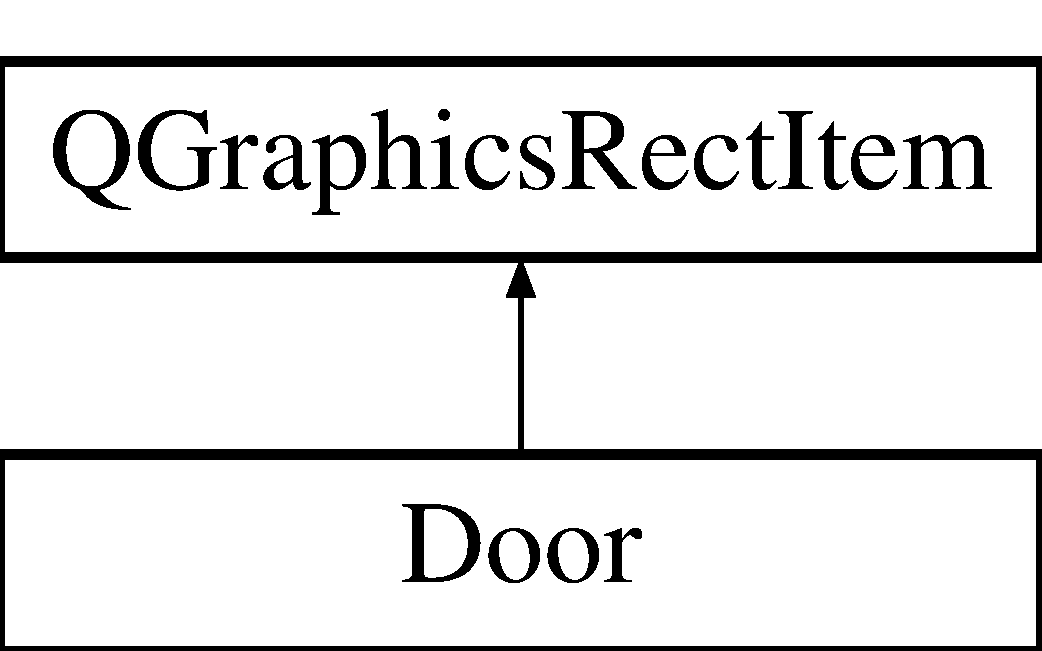
\includegraphics[height=2.000000cm]{classDoor}
\end{center}
\end{figure}
\subsection*{Public Member Functions}
\begin{DoxyCompactItemize}
\item 
\hyperlink{classDoor_a9a3828bd84f205da13c7591fafc29783}{Door} (qreal x, qreal y, qreal w, qreal h, Q\-Graphics\-Scene $\ast$scene)
\begin{DoxyCompactList}\small\item\em Constructor. \end{DoxyCompactList}\end{DoxyCompactItemize}


\subsection{Detailed Description}
The area which marks the end point of the game The \hyperlink{classDoor}{Door} is an object, which when a player touches, the player completes the game. 

\subsection{Constructor \& Destructor Documentation}
\hypertarget{classDoor_a9a3828bd84f205da13c7591fafc29783}{\index{Door@{Door}!Door@{Door}}
\index{Door@{Door}!Door@{Door}}
\subsubsection[{Door}]{\setlength{\rightskip}{0pt plus 5cm}Door\-::\-Door (
\begin{DoxyParamCaption}
\item[{qreal}]{x, }
\item[{qreal}]{y, }
\item[{qreal}]{w, }
\item[{qreal}]{h, }
\item[{Q\-Graphics\-Scene $\ast$}]{scene}
\end{DoxyParamCaption}
)}}\label{classDoor_a9a3828bd84f205da13c7591fafc29783}


Constructor. 


\begin{DoxyParams}{Parameters}
{\em x} & x coordinate \\
\hline
{\em y} & y coordinate \\
\hline
{\em w} & width \\
\hline
{\em h} & height \\
\hline
{\em scene} & the scene in which the door is drawn \\
\hline
\end{DoxyParams}


The documentation for this class was generated from the following file\-:\begin{DoxyCompactItemize}
\item 
door.\-h\end{DoxyCompactItemize}

\hypertarget{classEmptyInputComponent}{\section{Empty\-Input\-Component Class Reference}
\label{classEmptyInputComponent}\index{Empty\-Input\-Component@{Empty\-Input\-Component}}
}


\hyperlink{classInputComponent}{Input\-Component} for Game\-Objects that do not have any state changes.  




{\ttfamily \#include $<$emptyinputcomponent.\-h$>$}

Inheritance diagram for Empty\-Input\-Component\-:\begin{figure}[H]
\begin{center}
\leavevmode
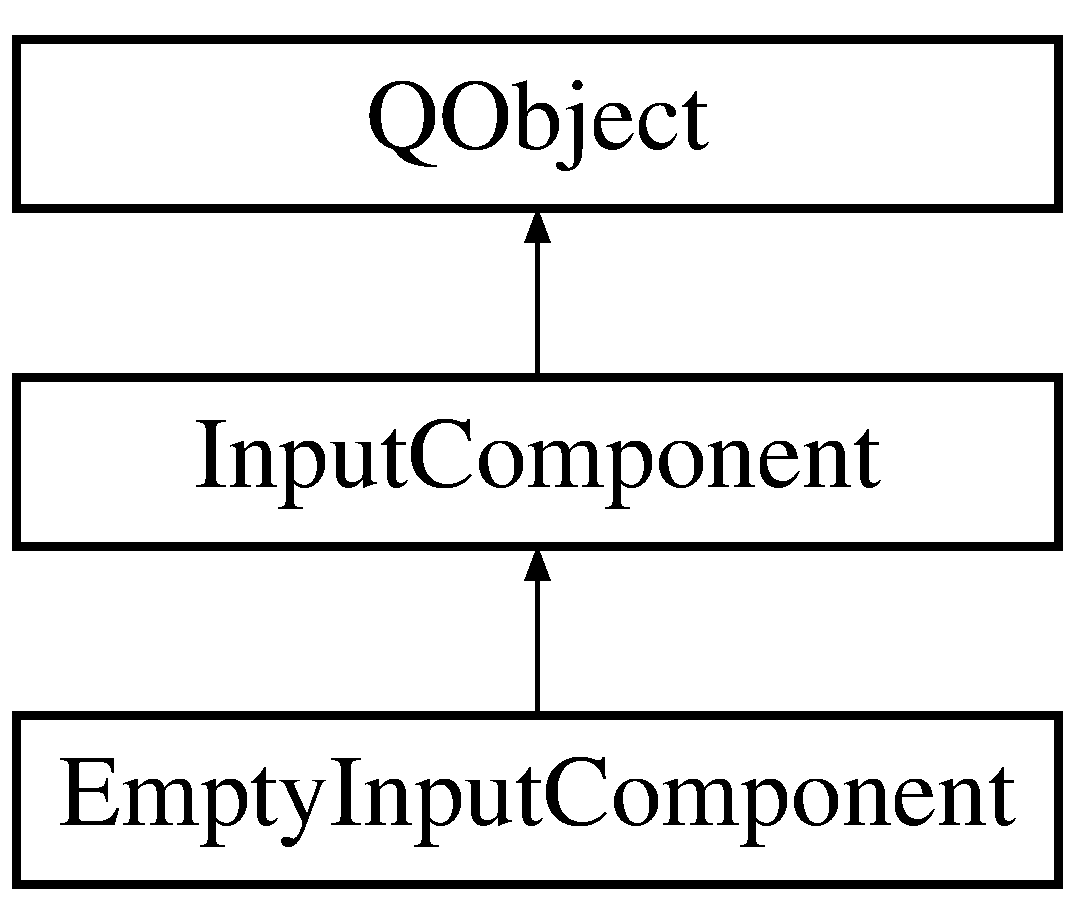
\includegraphics[height=3.000000cm]{classEmptyInputComponent}
\end{center}
\end{figure}
\subsection*{Public Member Functions}
\begin{DoxyCompactItemize}
\item 
\hypertarget{classEmptyInputComponent_a0d3cf59ff63535b73cdb90ce5764fde6}{\hyperlink{classEmptyInputComponent_a0d3cf59ff63535b73cdb90ce5764fde6}{Empty\-Input\-Component} ()}\label{classEmptyInputComponent_a0d3cf59ff63535b73cdb90ce5764fde6}

\begin{DoxyCompactList}\small\item\em Constructor. \end{DoxyCompactList}\item 
\hypertarget{classEmptyInputComponent_acf04a0a5e842522490a3f8ac05b8f896}{virtual \hyperlink{classEmptyInputComponent_acf04a0a5e842522490a3f8ac05b8f896}{$\sim$\-Empty\-Input\-Component} ()}\label{classEmptyInputComponent_acf04a0a5e842522490a3f8ac05b8f896}

\begin{DoxyCompactList}\small\item\em Destructor. \end{DoxyCompactList}\item 
virtual void \hyperlink{classEmptyInputComponent_a5e11b3048e027761e465072cda02a034}{update} (\hyperlink{classGameObject}{Game\-Object} \&game\-Object)
\begin{DoxyCompactList}\small\item\em updates the \hyperlink{classState}{State} of game\-Object \end{DoxyCompactList}\item 
virtual bool \hyperlink{classEmptyInputComponent_a821f567bd824806e2322f22ce5955b06}{accepts\-Input} ()
\begin{DoxyCompactList}\small\item\em Checks whether the \hyperlink{classGameObject}{Game\-Object} corresponding to this component accepts input. \end{DoxyCompactList}\end{DoxyCompactItemize}
\subsection*{Additional Inherited Members}


\subsection{Detailed Description}
\hyperlink{classInputComponent}{Input\-Component} for Game\-Objects that do not have any state changes. 

\subsection{Member Function Documentation}
\hypertarget{classEmptyInputComponent_a821f567bd824806e2322f22ce5955b06}{\index{Empty\-Input\-Component@{Empty\-Input\-Component}!accepts\-Input@{accepts\-Input}}
\index{accepts\-Input@{accepts\-Input}!EmptyInputComponent@{Empty\-Input\-Component}}
\subsubsection[{accepts\-Input}]{\setlength{\rightskip}{0pt plus 5cm}virtual bool Empty\-Input\-Component\-::accepts\-Input (
\begin{DoxyParamCaption}
{}
\end{DoxyParamCaption}
)\hspace{0.3cm}{\ttfamily [virtual]}}}\label{classEmptyInputComponent_a821f567bd824806e2322f22ce5955b06}


Checks whether the \hyperlink{classGameObject}{Game\-Object} corresponding to this component accepts input. 

\begin{DoxyReturn}{Returns}
false, as the component is empty 
\end{DoxyReturn}


Implements \hyperlink{classInputComponent_a27a4de99780ddf7d7a4f9d469f13640c}{Input\-Component}.

\hypertarget{classEmptyInputComponent_a5e11b3048e027761e465072cda02a034}{\index{Empty\-Input\-Component@{Empty\-Input\-Component}!update@{update}}
\index{update@{update}!EmptyInputComponent@{Empty\-Input\-Component}}
\subsubsection[{update}]{\setlength{\rightskip}{0pt plus 5cm}virtual void Empty\-Input\-Component\-::update (
\begin{DoxyParamCaption}
\item[{{\bf Game\-Object} \&}]{game\-Object}
\end{DoxyParamCaption}
)\hspace{0.3cm}{\ttfamily [virtual]}}}\label{classEmptyInputComponent_a5e11b3048e027761e465072cda02a034}


updates the \hyperlink{classState}{State} of game\-Object 


\begin{DoxyParams}{Parameters}
{\em game\-Object} & the \hyperlink{classGameObject}{Game\-Object} whose state is to be updated \\
\hline
\end{DoxyParams}


Implements \hyperlink{classInputComponent_a93e790f7279e842ee249fefe7dbf7b32}{Input\-Component}.



The documentation for this class was generated from the following file\-:\begin{DoxyCompactItemize}
\item 
emptyinputcomponent.\-h\end{DoxyCompactItemize}

\hypertarget{classEmptyPhysicsComponent}{\section{Empty\-Physics\-Component Class Reference}
\label{classEmptyPhysicsComponent}\index{Empty\-Physics\-Component@{Empty\-Physics\-Component}}
}


\hyperlink{classPhysicsComponent}{Physics\-Component} for Game\-Objects that do not move Used for objects such as Fire.  




{\ttfamily \#include $<$emptyphysicscomponent.\-h$>$}

Inheritance diagram for Empty\-Physics\-Component\-:\begin{figure}[H]
\begin{center}
\leavevmode
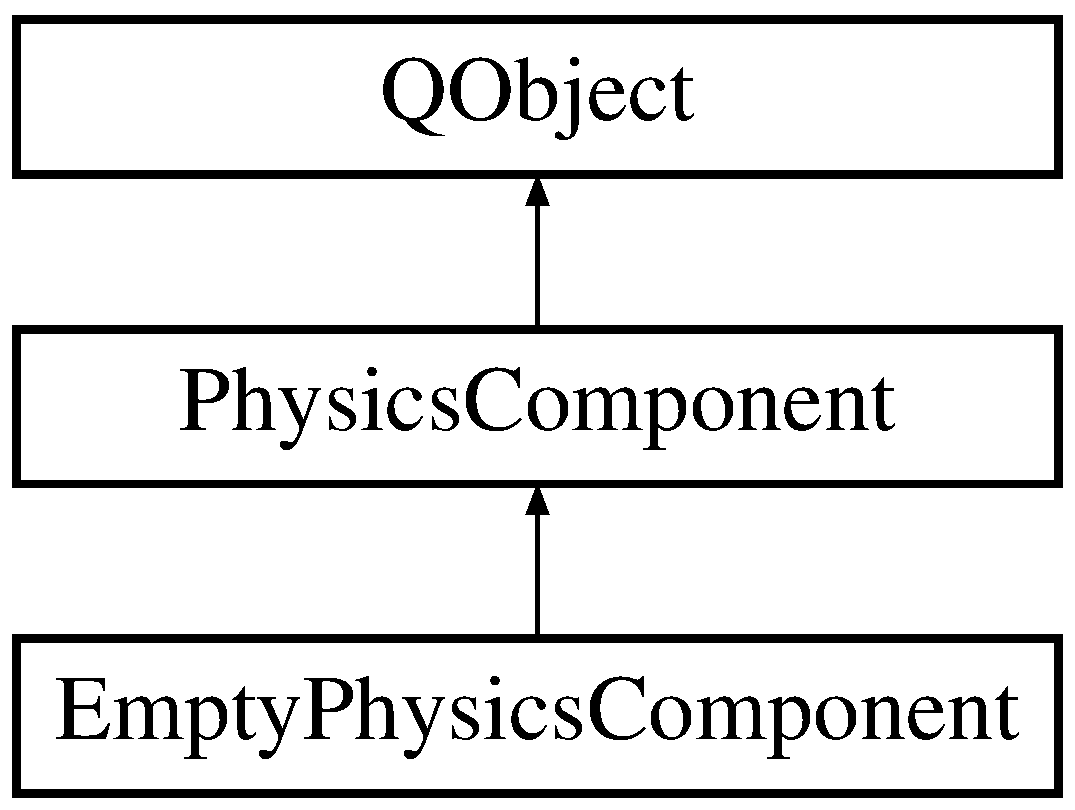
\includegraphics[height=3.000000cm]{classEmptyPhysicsComponent}
\end{center}
\end{figure}
\subsection*{Public Member Functions}
\begin{DoxyCompactItemize}
\item 
\hypertarget{classEmptyPhysicsComponent_af8b7cc144f6cf386168a6728329ee5af}{\hyperlink{classEmptyPhysicsComponent_af8b7cc144f6cf386168a6728329ee5af}{Empty\-Physics\-Component} ()}\label{classEmptyPhysicsComponent_af8b7cc144f6cf386168a6728329ee5af}

\begin{DoxyCompactList}\small\item\em Constructor. \end{DoxyCompactList}\item 
\hypertarget{classEmptyPhysicsComponent_ac2af2630a822087545750e0be469829f}{virtual \hyperlink{classEmptyPhysicsComponent_ac2af2630a822087545750e0be469829f}{$\sim$\-Empty\-Physics\-Component} ()}\label{classEmptyPhysicsComponent_ac2af2630a822087545750e0be469829f}

\begin{DoxyCompactList}\small\item\em Destructor. \end{DoxyCompactList}\item 
void \hyperlink{classEmptyPhysicsComponent_af1d5179fe8277973c4e1169ffc4f018d}{update} (\hyperlink{classGameObject}{Game\-Object} \&game\-Object)
\begin{DoxyCompactList}\small\item\em Updates the position of game\-Object. \end{DoxyCompactList}\end{DoxyCompactItemize}
\subsection*{Additional Inherited Members}


\subsection{Detailed Description}
\hyperlink{classPhysicsComponent}{Physics\-Component} for Game\-Objects that do not move Used for objects such as Fire. 

\subsection{Member Function Documentation}
\hypertarget{classEmptyPhysicsComponent_af1d5179fe8277973c4e1169ffc4f018d}{\index{Empty\-Physics\-Component@{Empty\-Physics\-Component}!update@{update}}
\index{update@{update}!EmptyPhysicsComponent@{Empty\-Physics\-Component}}
\subsubsection[{update}]{\setlength{\rightskip}{0pt plus 5cm}void Empty\-Physics\-Component\-::update (
\begin{DoxyParamCaption}
\item[{{\bf Game\-Object} \&}]{game\-Object}
\end{DoxyParamCaption}
)\hspace{0.3cm}{\ttfamily [virtual]}}}\label{classEmptyPhysicsComponent_af1d5179fe8277973c4e1169ffc4f018d}


Updates the position of game\-Object. 


\begin{DoxyParams}{Parameters}
{\em game\-Object} & the \hyperlink{classGameObject}{Game\-Object} whose position is to be updated \\
\hline
\end{DoxyParams}


Implements \hyperlink{classPhysicsComponent_a5498919fee09ce15271a5c273c2dc836}{Physics\-Component}.



The documentation for this class was generated from the following file\-:\begin{DoxyCompactItemize}
\item 
emptyphysicscomponent.\-h\end{DoxyCompactItemize}

\hypertarget{classFireGraphicsComponent}{\section{Fire\-Graphics\-Component Class Reference}
\label{classFireGraphicsComponent}\index{Fire\-Graphics\-Component@{Fire\-Graphics\-Component}}
}


The Graphics for fire objects This handles the drawing, placement, position and update of fire objects.  




{\ttfamily \#include $<$firegraphicscomponent.\-h$>$}

Inheritance diagram for Fire\-Graphics\-Component\-:\begin{figure}[H]
\begin{center}
\leavevmode
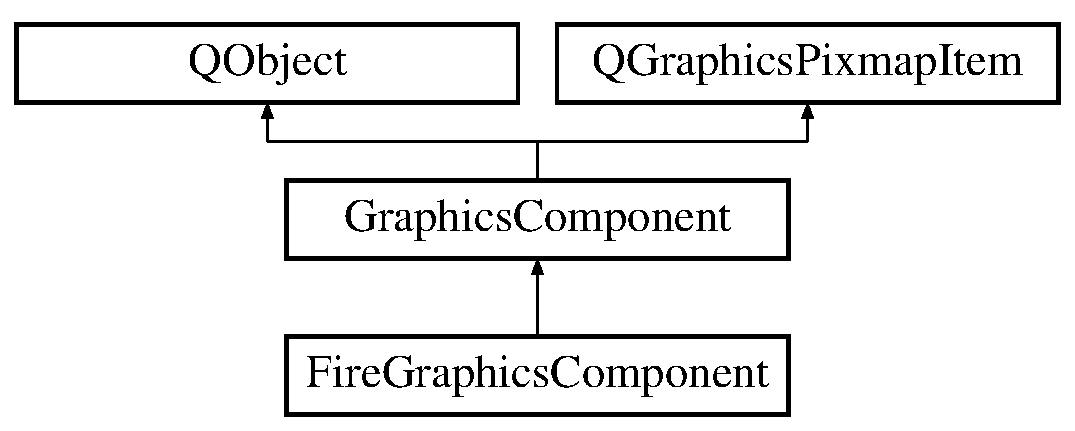
\includegraphics[height=3.000000cm]{classFireGraphicsComponent}
\end{center}
\end{figure}
\subsection*{Public Member Functions}
\begin{DoxyCompactItemize}
\item 
\hyperlink{classFireGraphicsComponent_a29253e498de59832c1cc2bd2f9bb11cc}{Fire\-Graphics\-Component} (Q\-Graphics\-Scene $\ast$scene, Q\-Pixmap $\ast$pix\-\_\-map, int images\-\_\-total\-\_\-count, qreal x\-\_\-coordinate, qreal y\-\_\-coordinate)
\begin{DoxyCompactList}\small\item\em Constructor. \end{DoxyCompactList}\item 
\hypertarget{classFireGraphicsComponent_a325c4a94a0208b9e640146f7a5dc68d0}{\hyperlink{classFireGraphicsComponent_a325c4a94a0208b9e640146f7a5dc68d0}{$\sim$\-Fire\-Graphics\-Component} ()}\label{classFireGraphicsComponent_a325c4a94a0208b9e640146f7a5dc68d0}

\begin{DoxyCompactList}\small\item\em Destructor. \end{DoxyCompactList}\item 
void \hyperlink{classFireGraphicsComponent_a241b7300febe73c29791803784d65c4a}{update} (\hyperlink{classGameObject}{Game\-Object} \&game\-Object)
\begin{DoxyCompactList}\small\item\em update Updates the image based on graphics\-Counter \end{DoxyCompactList}\item 
std\-::vector$<$ qreal $>$ \hyperlink{classFireGraphicsComponent_a61a1db833ae5aff3a0b4464d3a7d9761}{get\-Size\-Position\-Of\-Object} ()
\begin{DoxyCompactList}\small\item\em Gives the size and position of the \hyperlink{classGraphicsComponent}{Graphics\-Component} of the \hyperlink{classGameObject}{Game\-Object}. \end{DoxyCompactList}\end{DoxyCompactItemize}
\subsection*{Additional Inherited Members}


\subsection{Detailed Description}
The Graphics for fire objects This handles the drawing, placement, position and update of fire objects. 

\subsection{Constructor \& Destructor Documentation}
\hypertarget{classFireGraphicsComponent_a29253e498de59832c1cc2bd2f9bb11cc}{\index{Fire\-Graphics\-Component@{Fire\-Graphics\-Component}!Fire\-Graphics\-Component@{Fire\-Graphics\-Component}}
\index{Fire\-Graphics\-Component@{Fire\-Graphics\-Component}!FireGraphicsComponent@{Fire\-Graphics\-Component}}
\subsubsection[{Fire\-Graphics\-Component}]{\setlength{\rightskip}{0pt plus 5cm}Fire\-Graphics\-Component\-::\-Fire\-Graphics\-Component (
\begin{DoxyParamCaption}
\item[{Q\-Graphics\-Scene $\ast$}]{scene, }
\item[{Q\-Pixmap $\ast$}]{pix\-\_\-map, }
\item[{int}]{images\-\_\-total\-\_\-count, }
\item[{qreal}]{x\-\_\-coordinate, }
\item[{qreal}]{y\-\_\-coordinate}
\end{DoxyParamCaption}
)}}\label{classFireGraphicsComponent_a29253e498de59832c1cc2bd2f9bb11cc}


Constructor. 


\begin{DoxyParams}{Parameters}
{\em scene} & the scene where the fire is placed \\
\hline
{\em pix\-\_\-map} & Pixmap for the fire \\
\hline
{\em images\-\_\-total\-\_\-count} & number of images to be looped over \\
\hline
{\em x\-\_\-coordinate} & x coordinate of the position \\
\hline
{\em y\-\_\-coordinate} & y coordinate of the position \\
\hline
\end{DoxyParams}


\subsection{Member Function Documentation}
\hypertarget{classFireGraphicsComponent_a61a1db833ae5aff3a0b4464d3a7d9761}{\index{Fire\-Graphics\-Component@{Fire\-Graphics\-Component}!get\-Size\-Position\-Of\-Object@{get\-Size\-Position\-Of\-Object}}
\index{get\-Size\-Position\-Of\-Object@{get\-Size\-Position\-Of\-Object}!FireGraphicsComponent@{Fire\-Graphics\-Component}}
\subsubsection[{get\-Size\-Position\-Of\-Object}]{\setlength{\rightskip}{0pt plus 5cm}std\-::vector$<$qreal$>$ Fire\-Graphics\-Component\-::get\-Size\-Position\-Of\-Object (
\begin{DoxyParamCaption}
{}
\end{DoxyParamCaption}
)\hspace{0.3cm}{\ttfamily [virtual]}}}\label{classFireGraphicsComponent_a61a1db833ae5aff3a0b4464d3a7d9761}


Gives the size and position of the \hyperlink{classGraphicsComponent}{Graphics\-Component} of the \hyperlink{classGameObject}{Game\-Object}. 

\begin{DoxyReturn}{Returns}
a vector of type qreal, with width, height, x coordinate, y coordinate filled in that order 
\end{DoxyReturn}


Implements \hyperlink{classGraphicsComponent_a653e0474dd66fc1876f405831e121631}{Graphics\-Component}.

\hypertarget{classFireGraphicsComponent_a241b7300febe73c29791803784d65c4a}{\index{Fire\-Graphics\-Component@{Fire\-Graphics\-Component}!update@{update}}
\index{update@{update}!FireGraphicsComponent@{Fire\-Graphics\-Component}}
\subsubsection[{update}]{\setlength{\rightskip}{0pt plus 5cm}void Fire\-Graphics\-Component\-::update (
\begin{DoxyParamCaption}
\item[{{\bf Game\-Object} \&}]{game\-Object}
\end{DoxyParamCaption}
)\hspace{0.3cm}{\ttfamily [virtual]}}}\label{classFireGraphicsComponent_a241b7300febe73c29791803784d65c4a}


update Updates the image based on graphics\-Counter 


\begin{DoxyParams}{Parameters}
{\em game\-Object} & the \hyperlink{classGameObject}{Game\-Object} of the fire \\
\hline
\end{DoxyParams}


Reimplemented from \hyperlink{classGraphicsComponent_a744134b79cf11b2ff29fb7802923fda9}{Graphics\-Component}.



The documentation for this class was generated from the following file\-:\begin{DoxyCompactItemize}
\item 
firegraphicscomponent.\-h\end{DoxyCompactItemize}

\hypertarget{classGameObject}{\section{Game\-Object Class Reference}
\label{classGameObject}\index{Game\-Object@{Game\-Object}}
}


A Game Object This represents all the Game Objects in the game, including players, monsters and fire and the way to create them, display them, move them, and update state $\ast$.  




{\ttfamily \#include $<$gameobject.\-h$>$}

Inheritance diagram for Game\-Object\-:\begin{figure}[H]
\begin{center}
\leavevmode
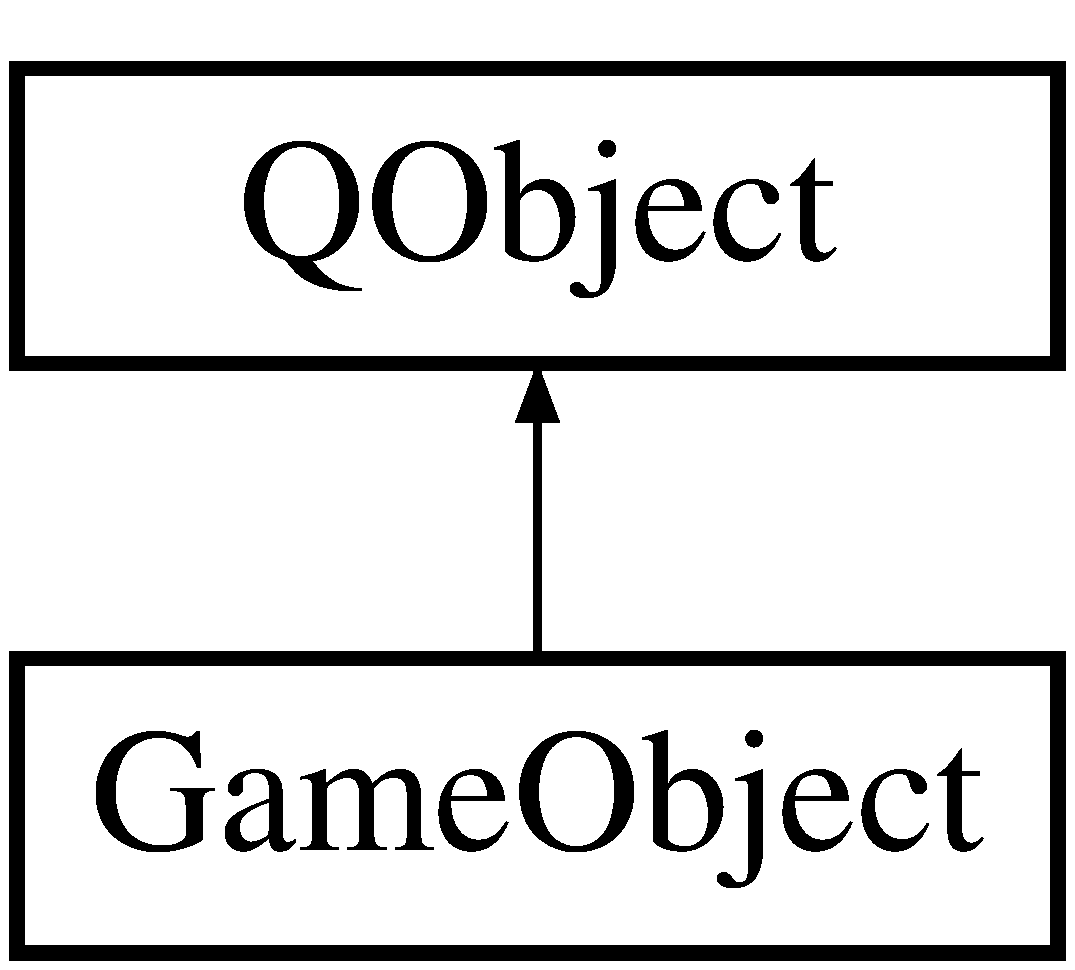
\includegraphics[height=2.000000cm]{classGameObject}
\end{center}
\end{figure}
\subsection*{Public Member Functions}
\begin{DoxyCompactItemize}
\item 
void \hyperlink{classGameObject_a461843e85bd8bfd205016e4adfd32489}{set\-Is\-Dead} (bool input)
\begin{DoxyCompactList}\small\item\em Sets the value of is\-Dead. \end{DoxyCompactList}\item 
bool \hyperlink{classGameObject_ab517f9caa5b662ec7ee8a8ead945ec8c}{get\-Is\-Dead} ()
\begin{DoxyCompactList}\small\item\em Get the value of is\-Dead. \end{DoxyCompactList}\item 
\hyperlink{namespaceenumerator_a74b6f7a3aada6983503ce0f88ee90b29}{enumerator\-::\-Object\-Type} \hyperlink{classGameObject_a5f4df627b722ca069bb497b83cb2cd47}{get\-Object\-Type} ()
\begin{DoxyCompactList}\small\item\em Get the value of objecttype. \end{DoxyCompactList}\item 
void \hyperlink{classGameObject_a20cc88a6d715503efcd3746d6aceb027}{set\-Object\-Type} (\hyperlink{namespaceenumerator_a74b6f7a3aada6983503ce0f88ee90b29}{enumerator\-::\-Object\-Type} input)
\begin{DoxyCompactList}\small\item\em Sets the value of objecttype. \end{DoxyCompactList}\item 
\hyperlink{classGameObject_a3a6bd333e736ddabb177574217f6a93b}{Game\-Object} (\hyperlink{classInputComponent}{Input\-Component} $\ast$input\-\_\-component, \hyperlink{classGraphicsComponent}{Graphics\-Component} $\ast$graphics\-\_\-component, \hyperlink{classPhysicsComponent}{Physics\-Component} $\ast$physics\-\_\-component, \hyperlink{classScoreComponent}{Score\-Component} $\ast$score\-\_\-component, const int \&max\-\_\-jump\-\_\-count, int time\-\_\-left=0)
\begin{DoxyCompactList}\small\item\em Constructor. \end{DoxyCompactList}\item 
\hypertarget{classGameObject_a224d4f6d9dd75c8a6f9d022eaf586fd9}{virtual \hyperlink{classGameObject_a224d4f6d9dd75c8a6f9d022eaf586fd9}{$\sim$\-Game\-Object} ()}\label{classGameObject_a224d4f6d9dd75c8a6f9d022eaf586fd9}

\begin{DoxyCompactList}\small\item\em Destructor. \end{DoxyCompactList}\item 
void \hyperlink{classGameObject_ae6c3730fbfc5fea46106466166177460}{set\-State} (\hyperlink{classState}{State} $\ast$input\-\_\-state)
\begin{DoxyCompactList}\small\item\em Sets the value of sate. \end{DoxyCompactList}\item 
void \hyperlink{classGameObject_a39aa8c311f514b871e6781bb076d8fdd}{set\-Jumping\-State} (\hyperlink{classJumpingState}{Jumping\-State} $\ast$input\-\_\-jumping\-\_\-state)
\begin{DoxyCompactList}\small\item\em Sets the value of jumping\-State. \end{DoxyCompactList}\item 
void \hyperlink{classGameObject_a23073437c24792019aac0b0663e93508}{set\-Score} (int input\-\_\-score)
\begin{DoxyCompactList}\small\item\em Sets the score of the \hyperlink{classGameObject}{Game\-Object}. \end{DoxyCompactList}\item 
int \hyperlink{classGameObject_a3bca3bee655746fb126bae49968d57fb}{get\-Score} ()
\begin{DoxyCompactList}\small\item\em Get the value of score. \end{DoxyCompactList}\item 
void \hyperlink{classGameObject_a9ecb58bea379eeb1d0b973b743861bf1}{set\-Name} (Q\-String name\-\_\-local)
\begin{DoxyCompactList}\small\item\em Sets the user name of the \hyperlink{classGameObject}{Game\-Object}, applies to players. \end{DoxyCompactList}\item 
Q\-String \hyperlink{classGameObject_a2dd3ed6457725c3b4730e93dd070f927}{get\-Name} ()
\begin{DoxyCompactList}\small\item\em Get the user name of the \hyperlink{classGameObject}{Game\-Object}, applies to players. \end{DoxyCompactList}\item 
int \hyperlink{classGameObject_a12af00f8b80f69e679e00c75b237a11c}{get\-Time\-Left} ()
\begin{DoxyCompactList}\small\item\em Get the time left for the \hyperlink{classGameObject}{Game\-Object} in the game, applies to players. \end{DoxyCompactList}\item 
bool \hyperlink{classGameObject_a6fc32284114a6d3b45c3d0485c688146}{is\-Accepting\-Input} ()
\begin{DoxyCompactList}\small\item\em Get whether the \hyperlink{classGameObject}{Game\-Object} accepts input from the keyboard. \end{DoxyCompactList}\item 
void \hyperlink{classGameObject_a9271d8661100d433a104601cd0d0d891}{set\-Accepting\-Input} (bool value)
\begin{DoxyCompactList}\small\item\em Set whether the \hyperlink{classGameObject}{Game\-Object} accepts input from the keyboard. \end{DoxyCompactList}\item 
void \hyperlink{classGameObject_ab10b02b28281e7398cd9f05bb7bea9c3}{set\-Pos\-X\-Y} (Q\-Point\-F point)
\begin{DoxyCompactList}\small\item\em Set the position of the \hyperlink{classGameObject}{Game\-Object} in the next frame. \end{DoxyCompactList}\item 
Q\-Point\-F \hyperlink{classGameObject_ae4529f9eeec4153ee11ff685d5c4443b}{get\-Pos\-X\-Y} ()
\begin{DoxyCompactList}\small\item\em Get the position where the \hyperlink{classGameObject}{Game\-Object} will go in the next frame. \end{DoxyCompactList}\item 
\hypertarget{classGameObject_a13fe91332392ef175ed61e57e9414111}{void \hyperlink{classGameObject_a13fe91332392ef175ed61e57e9414111}{update\-Pos} ()}\label{classGameObject_a13fe91332392ef175ed61e57e9414111}

\begin{DoxyCompactList}\small\item\em Update the position of the player. \end{DoxyCompactList}\end{DoxyCompactItemize}
\subsection*{Public Attributes}
\begin{DoxyCompactItemize}
\item 
\hypertarget{classGameObject_a05bfcec90c5fd5579ae901ad09919b12}{Q\-String \hyperlink{classGameObject_a05bfcec90c5fd5579ae901ad09919b12}{name}}\label{classGameObject_a05bfcec90c5fd5579ae901ad09919b12}

\begin{DoxyCompactList}\small\item\em Stores the username, applies to players. \end{DoxyCompactList}\item 
\hypertarget{classGameObject_a6ca856e43814c856465e252c2620b4fd}{int \hyperlink{classGameObject_a6ca856e43814c856465e252c2620b4fd}{time\-Left}}\label{classGameObject_a6ca856e43814c856465e252c2620b4fd}

\begin{DoxyCompactList}\small\item\em Stores the time left when the player completed the game, applies to players. \end{DoxyCompactList}\item 
\hypertarget{classGameObject_a32194bfeb8fa7c182b461b3d81f5b4f8}{const int \hyperlink{classGameObject_a32194bfeb8fa7c182b461b3d81f5b4f8}{max\-Jump\-Count}}\label{classGameObject_a32194bfeb8fa7c182b461b3d81f5b4f8}

\begin{DoxyCompactList}\small\item\em Specifies the number of frames the \hyperlink{classGameObject}{Game\-Object} moves up on jumping. \end{DoxyCompactList}\item 
\hypertarget{classGameObject_a5d0f552ee77c70c8f28b11dd792bf5e9}{\hyperlink{classInputComponent}{Input\-Component} $\ast$ \hyperlink{classGameObject_a5d0f552ee77c70c8f28b11dd792bf5e9}{input\-Component}}\label{classGameObject_a5d0f552ee77c70c8f28b11dd792bf5e9}

\begin{DoxyCompactList}\small\item\em Component that handles input Handles keyboard input and state changes of the \hyperlink{classGameObject}{Game\-Object}, and sets states appropriately. \end{DoxyCompactList}\item 
\hypertarget{classGameObject_abb548a6a6010953cded6906801ef4d2b}{\hyperlink{classGraphicsComponent}{Graphics\-Component} $\ast$ \hyperlink{classGameObject_abb548a6a6010953cded6906801ef4d2b}{graphics\-Component}}\label{classGameObject_abb548a6a6010953cded6906801ef4d2b}

\begin{DoxyCompactList}\small\item\em Component that handles graphics Handles the drawing of the \hyperlink{classGameObject}{Game\-Object} on the sceen, stores how it is drawn, and updates based on state. \end{DoxyCompactList}\item 
\hypertarget{classGameObject_a670ef0bb2154d5941a3da1c8ed45a0b8}{\hyperlink{classPhysicsComponent}{Physics\-Component} $\ast$ \hyperlink{classGameObject_a670ef0bb2154d5941a3da1c8ed45a0b8}{physics\-Component}}\label{classGameObject_a670ef0bb2154d5941a3da1c8ed45a0b8}

\begin{DoxyCompactList}\small\item\em Component that handles physics Handles the movement of \hyperlink{classGameObject}{Game\-Object} based on the current state, and updates the current position on the scene. \end{DoxyCompactList}\item 
\hypertarget{classGameObject_a944d6d66cb7b92a474a4fe35a477897d}{\hyperlink{classScoreComponent}{Score\-Component} $\ast$ \hyperlink{classGameObject_a944d6d66cb7b92a474a4fe35a477897d}{score\-Component}}\label{classGameObject_a944d6d66cb7b92a474a4fe35a477897d}

\begin{DoxyCompactList}\small\item\em Component that handles score Handles the score of the \hyperlink{classGameObject}{Game\-Object}, the display of the score, and updates the score. Applies to players. \end{DoxyCompactList}\item 
\hypertarget{classGameObject_a787f40d5aee7507cdd6b8bb61dd8c19f}{\hyperlink{classState}{State} $\ast$ \hyperlink{classGameObject_a787f40d5aee7507cdd6b8bb61dd8c19f}{state}}\label{classGameObject_a787f40d5aee7507cdd6b8bb61dd8c19f}

\begin{DoxyCompactList}\small\item\em \hyperlink{classState}{State} of the \hyperlink{classGameObject}{Game\-Object} Stores the state of the \hyperlink{classGameObject}{Game\-Object}, in particular the state of its motion in the x direction Includes Moving Left, Moving Right, Stationary facing left, Stationary facing right Dead facing left, Dead facing right Also handles changes to the state based on the current key combination. \end{DoxyCompactList}\item 
\hypertarget{classGameObject_a980519676ac2aa7768729c01d768dad7}{\hyperlink{classJumpingState}{Jumping\-State} $\ast$ \hyperlink{classGameObject_a980519676ac2aa7768729c01d768dad7}{jumping\-State}}\label{classGameObject_a980519676ac2aa7768729c01d768dad7}

\begin{DoxyCompactList}\small\item\em Jumping \hyperlink{classState}{State} of the \hyperlink{classGameObject}{Game\-Object} Stores the Jumping \hyperlink{classState}{State} of the \hyperlink{classGameObject}{Game\-Object}, and consists of \hyperlink{classIsJumping}{Is\-Jumping} and \hyperlink{classIsNotJumping}{Is\-Not\-Jumping} Also handles changes to the \hyperlink{classJumpingState}{Jumping\-State} based on the current key combination. \end{DoxyCompactList}\end{DoxyCompactItemize}
\subsection*{Protected Attributes}
\begin{DoxyCompactItemize}
\item 
\hypertarget{classGameObject_a5711f465dd7765919f5d8fe21673aaa3}{bool \hyperlink{classGameObject_a5711f465dd7765919f5d8fe21673aaa3}{accepts\-Input}}\label{classGameObject_a5711f465dd7765919f5d8fe21673aaa3}

\begin{DoxyCompactList}\small\item\em Specifies whether the \hyperlink{classGameObject}{Game\-Object} accepts keyboard input. \end{DoxyCompactList}\item 
\hypertarget{classGameObject_af684f5c351429efdb3bf376eba3beaf9}{bool \hyperlink{classGameObject_af684f5c351429efdb3bf376eba3beaf9}{is\-Dead}}\label{classGameObject_af684f5c351429efdb3bf376eba3beaf9}

\begin{DoxyCompactList}\small\item\em Specifies whether the \hyperlink{classGameObject}{Game\-Object} is alive, applicable to players. \end{DoxyCompactList}\item 
\hypertarget{classGameObject_ac4a4836d4e250af380475bf0791c4234}{\hyperlink{namespaceenumerator_a74b6f7a3aada6983503ce0f88ee90b29}{enumerator\-::\-Object\-Type} \hyperlink{classGameObject_ac4a4836d4e250af380475bf0791c4234}{objecttype}}\label{classGameObject_ac4a4836d4e250af380475bf0791c4234}

\begin{DoxyCompactList}\small\item\em Specifies whether the \hyperlink{classGameObject}{Game\-Object} is a player or a monster, value undefined otherwise. \end{DoxyCompactList}\item 
\hypertarget{classGameObject_a282f206512274bde89acc9b1a5870e6e}{int \hyperlink{classGameObject_a282f206512274bde89acc9b1a5870e6e}{score}}\label{classGameObject_a282f206512274bde89acc9b1a5870e6e}

\begin{DoxyCompactList}\small\item\em Specifies the score of the \hyperlink{classGameObject}{Game\-Object}, applicable to players. \end{DoxyCompactList}\item 
\hypertarget{classGameObject_a80707284fe2dfb659cbf6d5602033fc4}{qreal \hyperlink{classGameObject_a80707284fe2dfb659cbf6d5602033fc4}{set\-Pos\-X}}\label{classGameObject_a80707284fe2dfb659cbf6d5602033fc4}

\begin{DoxyCompactList}\small\item\em Specifies x coordinate where the \hyperlink{classGameObject}{Game\-Object} needs to be placed in the next frame. \end{DoxyCompactList}\item 
\hypertarget{classGameObject_a3fb32317c043ba8cc2dc4744d5ff463a}{qreal \hyperlink{classGameObject_a3fb32317c043ba8cc2dc4744d5ff463a}{set\-Pos\-Y}}\label{classGameObject_a3fb32317c043ba8cc2dc4744d5ff463a}

\begin{DoxyCompactList}\small\item\em Specifies y coordinate where the \hyperlink{classGameObject}{Game\-Object} needs to be placed in the next frame. \end{DoxyCompactList}\end{DoxyCompactItemize}


\subsection{Detailed Description}
A Game Object This represents all the Game Objects in the game, including players, monsters and fire and the way to create them, display them, move them, and update state $\ast$. 

\subsection{Constructor \& Destructor Documentation}
\hypertarget{classGameObject_a3a6bd333e736ddabb177574217f6a93b}{\index{Game\-Object@{Game\-Object}!Game\-Object@{Game\-Object}}
\index{Game\-Object@{Game\-Object}!GameObject@{Game\-Object}}
\subsubsection[{Game\-Object}]{\setlength{\rightskip}{0pt plus 5cm}Game\-Object\-::\-Game\-Object (
\begin{DoxyParamCaption}
\item[{{\bf Input\-Component} $\ast$}]{input\-\_\-component, }
\item[{{\bf Graphics\-Component} $\ast$}]{graphics\-\_\-component, }
\item[{{\bf Physics\-Component} $\ast$}]{physics\-\_\-component, }
\item[{{\bf Score\-Component} $\ast$}]{score\-\_\-component, }
\item[{const int \&}]{max\-\_\-jump\-\_\-count, }
\item[{int}]{time\-\_\-left = {\ttfamily 0}}
\end{DoxyParamCaption}
)}}\label{classGameObject_a3a6bd333e736ddabb177574217f6a93b}


Constructor. 


\begin{DoxyParams}{Parameters}
{\em input\-\_\-component} & value of input\-Component \\
\hline
{\em graphics\-\_\-component} & value of graphics\-Component \\
\hline
{\em physics\-\_\-component} & value of physics\-Component \\
\hline
{\em score\-\_\-component} & value of score\-Component \\
\hline
{\em max\-\_\-jump\-\_\-count} & value of max\-Jump\-Count \\
\hline
{\em time\-\_\-left} & time available for the \hyperlink{classGameObject}{Game\-Object} to play in the game when started \\
\hline
\end{DoxyParams}


\subsection{Member Function Documentation}
\hypertarget{classGameObject_ab517f9caa5b662ec7ee8a8ead945ec8c}{\index{Game\-Object@{Game\-Object}!get\-Is\-Dead@{get\-Is\-Dead}}
\index{get\-Is\-Dead@{get\-Is\-Dead}!GameObject@{Game\-Object}}
\subsubsection[{get\-Is\-Dead}]{\setlength{\rightskip}{0pt plus 5cm}bool Game\-Object\-::get\-Is\-Dead (
\begin{DoxyParamCaption}
{}
\end{DoxyParamCaption}
)}}\label{classGameObject_ab517f9caa5b662ec7ee8a8ead945ec8c}


Get the value of is\-Dead. 

\begin{DoxyReturn}{Returns}
value of is\-Dead 
\end{DoxyReturn}
\hypertarget{classGameObject_a2dd3ed6457725c3b4730e93dd070f927}{\index{Game\-Object@{Game\-Object}!get\-Name@{get\-Name}}
\index{get\-Name@{get\-Name}!GameObject@{Game\-Object}}
\subsubsection[{get\-Name}]{\setlength{\rightskip}{0pt plus 5cm}Q\-String Game\-Object\-::get\-Name (
\begin{DoxyParamCaption}
{}
\end{DoxyParamCaption}
)}}\label{classGameObject_a2dd3ed6457725c3b4730e93dd070f927}


Get the user name of the \hyperlink{classGameObject}{Game\-Object}, applies to players. 

\begin{DoxyReturn}{Returns}
the value of the user name 
\end{DoxyReturn}
\hypertarget{classGameObject_a5f4df627b722ca069bb497b83cb2cd47}{\index{Game\-Object@{Game\-Object}!get\-Object\-Type@{get\-Object\-Type}}
\index{get\-Object\-Type@{get\-Object\-Type}!GameObject@{Game\-Object}}
\subsubsection[{get\-Object\-Type}]{\setlength{\rightskip}{0pt plus 5cm}{\bf enumerator\-::\-Object\-Type} Game\-Object\-::get\-Object\-Type (
\begin{DoxyParamCaption}
{}
\end{DoxyParamCaption}
)}}\label{classGameObject_a5f4df627b722ca069bb497b83cb2cd47}


Get the value of objecttype. 

\begin{DoxyReturn}{Returns}
value of objecttype 
\end{DoxyReturn}
\hypertarget{classGameObject_ae4529f9eeec4153ee11ff685d5c4443b}{\index{Game\-Object@{Game\-Object}!get\-Pos\-X\-Y@{get\-Pos\-X\-Y}}
\index{get\-Pos\-X\-Y@{get\-Pos\-X\-Y}!GameObject@{Game\-Object}}
\subsubsection[{get\-Pos\-X\-Y}]{\setlength{\rightskip}{0pt plus 5cm}Q\-Point\-F Game\-Object\-::get\-Pos\-X\-Y (
\begin{DoxyParamCaption}
{}
\end{DoxyParamCaption}
)}}\label{classGameObject_ae4529f9eeec4153ee11ff685d5c4443b}


Get the position where the \hyperlink{classGameObject}{Game\-Object} will go in the next frame. 

\begin{DoxyReturn}{Returns}
the point 
\end{DoxyReturn}
\hypertarget{classGameObject_a3bca3bee655746fb126bae49968d57fb}{\index{Game\-Object@{Game\-Object}!get\-Score@{get\-Score}}
\index{get\-Score@{get\-Score}!GameObject@{Game\-Object}}
\subsubsection[{get\-Score}]{\setlength{\rightskip}{0pt plus 5cm}int Game\-Object\-::get\-Score (
\begin{DoxyParamCaption}
{}
\end{DoxyParamCaption}
)}}\label{classGameObject_a3bca3bee655746fb126bae49968d57fb}


Get the value of score. 

\begin{DoxyReturn}{Returns}
the value of score 
\end{DoxyReturn}
\hypertarget{classGameObject_a12af00f8b80f69e679e00c75b237a11c}{\index{Game\-Object@{Game\-Object}!get\-Time\-Left@{get\-Time\-Left}}
\index{get\-Time\-Left@{get\-Time\-Left}!GameObject@{Game\-Object}}
\subsubsection[{get\-Time\-Left}]{\setlength{\rightskip}{0pt plus 5cm}int Game\-Object\-::get\-Time\-Left (
\begin{DoxyParamCaption}
{}
\end{DoxyParamCaption}
)}}\label{classGameObject_a12af00f8b80f69e679e00c75b237a11c}


Get the time left for the \hyperlink{classGameObject}{Game\-Object} in the game, applies to players. 

\begin{DoxyReturn}{Returns}
the value of the time left 
\end{DoxyReturn}
\hypertarget{classGameObject_a6fc32284114a6d3b45c3d0485c688146}{\index{Game\-Object@{Game\-Object}!is\-Accepting\-Input@{is\-Accepting\-Input}}
\index{is\-Accepting\-Input@{is\-Accepting\-Input}!GameObject@{Game\-Object}}
\subsubsection[{is\-Accepting\-Input}]{\setlength{\rightskip}{0pt plus 5cm}bool Game\-Object\-::is\-Accepting\-Input (
\begin{DoxyParamCaption}
{}
\end{DoxyParamCaption}
)}}\label{classGameObject_a6fc32284114a6d3b45c3d0485c688146}


Get whether the \hyperlink{classGameObject}{Game\-Object} accepts input from the keyboard. 

\begin{DoxyReturn}{Returns}
true, if the \hyperlink{classGameObject}{Game\-Object} accepts input, false otherwise 
\end{DoxyReturn}
\hypertarget{classGameObject_a9271d8661100d433a104601cd0d0d891}{\index{Game\-Object@{Game\-Object}!set\-Accepting\-Input@{set\-Accepting\-Input}}
\index{set\-Accepting\-Input@{set\-Accepting\-Input}!GameObject@{Game\-Object}}
\subsubsection[{set\-Accepting\-Input}]{\setlength{\rightskip}{0pt plus 5cm}void Game\-Object\-::set\-Accepting\-Input (
\begin{DoxyParamCaption}
\item[{bool}]{value}
\end{DoxyParamCaption}
)}}\label{classGameObject_a9271d8661100d433a104601cd0d0d891}


Set whether the \hyperlink{classGameObject}{Game\-Object} accepts input from the keyboard. 


\begin{DoxyParams}{Parameters}
{\em value} & the new value, true if it accepts, false otherwise \\
\hline
\end{DoxyParams}
\hypertarget{classGameObject_a461843e85bd8bfd205016e4adfd32489}{\index{Game\-Object@{Game\-Object}!set\-Is\-Dead@{set\-Is\-Dead}}
\index{set\-Is\-Dead@{set\-Is\-Dead}!GameObject@{Game\-Object}}
\subsubsection[{set\-Is\-Dead}]{\setlength{\rightskip}{0pt plus 5cm}void Game\-Object\-::set\-Is\-Dead (
\begin{DoxyParamCaption}
\item[{bool}]{input}
\end{DoxyParamCaption}
)}}\label{classGameObject_a461843e85bd8bfd205016e4adfd32489}


Sets the value of is\-Dead. 


\begin{DoxyParams}{Parameters}
{\em input} & the new value of is\-Dead \\
\hline
\end{DoxyParams}
\hypertarget{classGameObject_a39aa8c311f514b871e6781bb076d8fdd}{\index{Game\-Object@{Game\-Object}!set\-Jumping\-State@{set\-Jumping\-State}}
\index{set\-Jumping\-State@{set\-Jumping\-State}!GameObject@{Game\-Object}}
\subsubsection[{set\-Jumping\-State}]{\setlength{\rightskip}{0pt plus 5cm}void Game\-Object\-::set\-Jumping\-State (
\begin{DoxyParamCaption}
\item[{{\bf Jumping\-State} $\ast$}]{input\-\_\-jumping\-\_\-state}
\end{DoxyParamCaption}
)}}\label{classGameObject_a39aa8c311f514b871e6781bb076d8fdd}


Sets the value of jumping\-State. 


\begin{DoxyParams}{Parameters}
{\em input\-\_\-jumping\-\_\-state} & the new value of jumping\-State \\
\hline
\end{DoxyParams}
\hypertarget{classGameObject_a9ecb58bea379eeb1d0b973b743861bf1}{\index{Game\-Object@{Game\-Object}!set\-Name@{set\-Name}}
\index{set\-Name@{set\-Name}!GameObject@{Game\-Object}}
\subsubsection[{set\-Name}]{\setlength{\rightskip}{0pt plus 5cm}void Game\-Object\-::set\-Name (
\begin{DoxyParamCaption}
\item[{Q\-String}]{name\-\_\-local}
\end{DoxyParamCaption}
)}}\label{classGameObject_a9ecb58bea379eeb1d0b973b743861bf1}


Sets the user name of the \hyperlink{classGameObject}{Game\-Object}, applies to players. 


\begin{DoxyParams}{Parameters}
{\em name\-\_\-local} & the new value of the user name \\
\hline
\end{DoxyParams}
\hypertarget{classGameObject_a20cc88a6d715503efcd3746d6aceb027}{\index{Game\-Object@{Game\-Object}!set\-Object\-Type@{set\-Object\-Type}}
\index{set\-Object\-Type@{set\-Object\-Type}!GameObject@{Game\-Object}}
\subsubsection[{set\-Object\-Type}]{\setlength{\rightskip}{0pt plus 5cm}void Game\-Object\-::set\-Object\-Type (
\begin{DoxyParamCaption}
\item[{{\bf enumerator\-::\-Object\-Type}}]{input}
\end{DoxyParamCaption}
)}}\label{classGameObject_a20cc88a6d715503efcd3746d6aceb027}


Sets the value of objecttype. 


\begin{DoxyParams}{Parameters}
{\em input} & the new value of objecttype \\
\hline
\end{DoxyParams}
\hypertarget{classGameObject_ab10b02b28281e7398cd9f05bb7bea9c3}{\index{Game\-Object@{Game\-Object}!set\-Pos\-X\-Y@{set\-Pos\-X\-Y}}
\index{set\-Pos\-X\-Y@{set\-Pos\-X\-Y}!GameObject@{Game\-Object}}
\subsubsection[{set\-Pos\-X\-Y}]{\setlength{\rightskip}{0pt plus 5cm}void Game\-Object\-::set\-Pos\-X\-Y (
\begin{DoxyParamCaption}
\item[{Q\-Point\-F}]{point}
\end{DoxyParamCaption}
)}}\label{classGameObject_ab10b02b28281e7398cd9f05bb7bea9c3}


Set the position of the \hyperlink{classGameObject}{Game\-Object} in the next frame. 


\begin{DoxyParams}{Parameters}
{\em point} & the point to which the \hyperlink{classGameObject}{Game\-Object} must go the next frame \\
\hline
\end{DoxyParams}
\hypertarget{classGameObject_a23073437c24792019aac0b0663e93508}{\index{Game\-Object@{Game\-Object}!set\-Score@{set\-Score}}
\index{set\-Score@{set\-Score}!GameObject@{Game\-Object}}
\subsubsection[{set\-Score}]{\setlength{\rightskip}{0pt plus 5cm}void Game\-Object\-::set\-Score (
\begin{DoxyParamCaption}
\item[{int}]{input\-\_\-score}
\end{DoxyParamCaption}
)}}\label{classGameObject_a23073437c24792019aac0b0663e93508}


Sets the score of the \hyperlink{classGameObject}{Game\-Object}. 


\begin{DoxyParams}{Parameters}
{\em input\-\_\-score} & the new value of score \\
\hline
\end{DoxyParams}
\hypertarget{classGameObject_ae6c3730fbfc5fea46106466166177460}{\index{Game\-Object@{Game\-Object}!set\-State@{set\-State}}
\index{set\-State@{set\-State}!GameObject@{Game\-Object}}
\subsubsection[{set\-State}]{\setlength{\rightskip}{0pt plus 5cm}void Game\-Object\-::set\-State (
\begin{DoxyParamCaption}
\item[{{\bf State} $\ast$}]{input\-\_\-state}
\end{DoxyParamCaption}
)}}\label{classGameObject_ae6c3730fbfc5fea46106466166177460}


Sets the value of sate. 


\begin{DoxyParams}{Parameters}
{\em input\-\_\-state} & the new value of state \\
\hline
\end{DoxyParams}


The documentation for this class was generated from the following file\-:\begin{DoxyCompactItemize}
\item 
gameobject.\-h\end{DoxyCompactItemize}

\hypertarget{classGameState}{\section{Game\-State Class Reference}
\label{classGameState}\index{Game\-State@{Game\-State}}
}


The state of the Game Stores the state of the game. Stores all the \hyperlink{classGameObject}{Game\-Object} members, \hyperlink{classGem}{Gem} members, tile map, and handles update of state.  




{\ttfamily \#include $<$gamestate.\-h$>$}

Inheritance diagram for Game\-State\-:\begin{figure}[H]
\begin{center}
\leavevmode
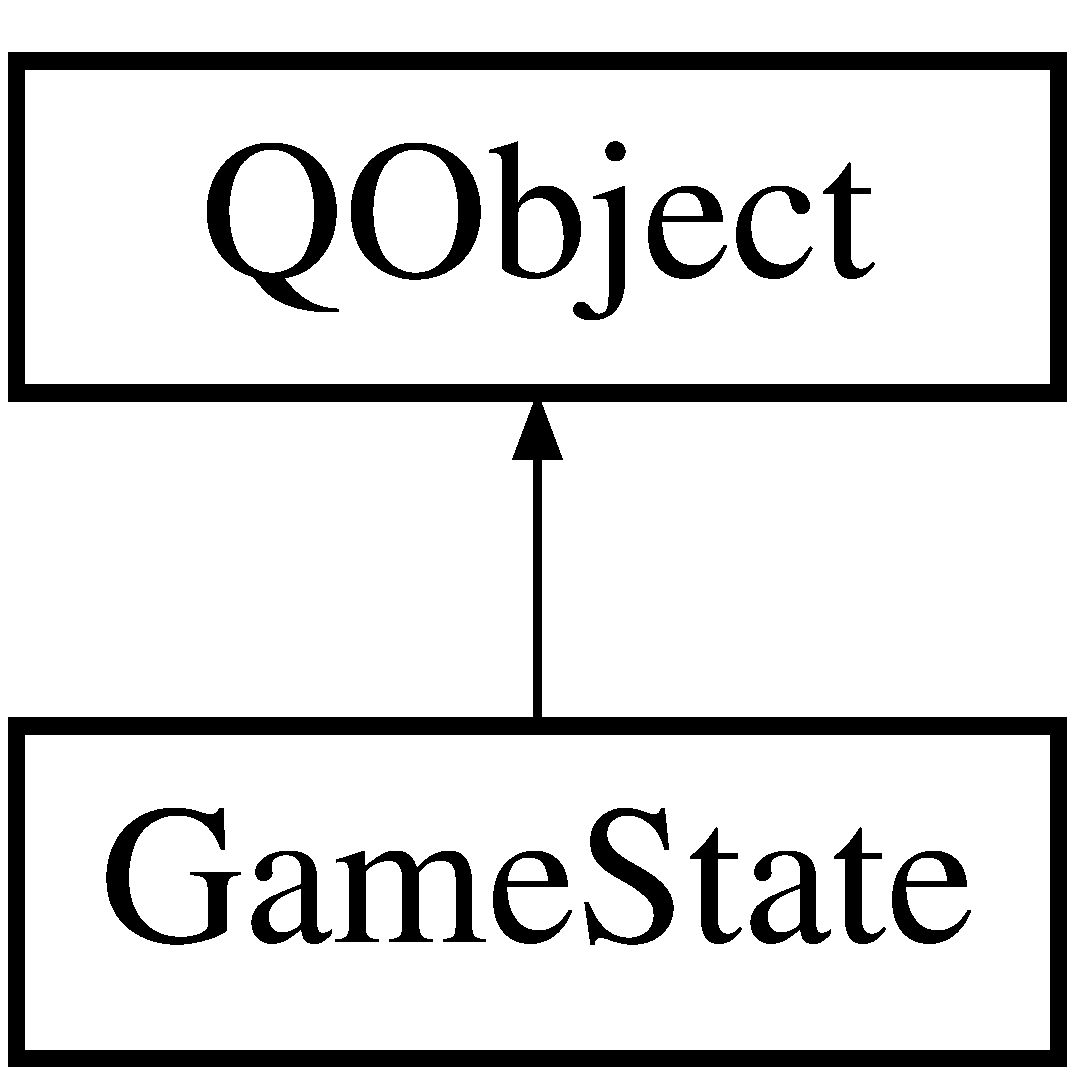
\includegraphics[height=2.000000cm]{classGameState}
\end{center}
\end{figure}
\subsection*{Public Slots}
\begin{DoxyCompactItemize}
\item 
\hypertarget{classGameState_aaecebaa5f6cd88e093927fc3cb321c10}{void \hyperlink{classGameState_aaecebaa5f6cd88e093927fc3cb321c10}{update} ()}\label{classGameState_aaecebaa5f6cd88e093927fc3cb321c10}

\begin{DoxyCompactList}\small\item\em Updates the state of the game Calls update on all the \hyperlink{classGameObject}{Game\-Object} objects, \hyperlink{classGem}{Gem} objects, \hyperlink{classTimer}{Timer}, such that the game moves forward my one frame Called once every frame. \end{DoxyCompactList}\end{DoxyCompactItemize}
\subsection*{Public Member Functions}
\begin{DoxyCompactItemize}
\item 
\hyperlink{classGameState_a284d3408e9b687a5c8c0072753d2e025}{Game\-State} (std\-::vector$<$ \hyperlink{classGameObject}{Game\-Object} $\ast$ $>$ \&game\-\_\-objects, std\-::vector$<$ std\-::vector$<$ \hyperlink{classTile}{Tile} $\ast$ $>$ $>$ \&tile\-\_\-map, std\-::vector$<$ \hyperlink{classGem}{Gem} $\ast$ $>$ \&input\-\_\-gems, int screen\-\_\-width, int screen\-\_\-height, Q\-Graphics\-Scene $\ast$scene\-\_\-local, int milliseconds\-\_\-per\-\_\-frame, int total\-\_\-time\-\_\-available)
\begin{DoxyCompactList}\small\item\em Constructor. \end{DoxyCompactList}\item 
\hypertarget{classGameState_a517ef6eaba96896259fcefd0c66afc9e}{virtual \hyperlink{classGameState_a517ef6eaba96896259fcefd0c66afc9e}{$\sim$\-Game\-State} ()}\label{classGameState_a517ef6eaba96896259fcefd0c66afc9e}

\begin{DoxyCompactList}\small\item\em Destructor. \end{DoxyCompactList}\item 
Q\-Graphics\-Scene $\ast$ \hyperlink{classGameState_af38b3925bdf2592414fe6276106553bb}{get\-Scene} ()
\begin{DoxyCompactList}\small\item\em Get the scene in which the game is being played. \end{DoxyCompactList}\item 
bool \hyperlink{classGameState_aeb4c715344671e22d6512d5e8dc12ffe}{is\-Game\-Active} ()
\begin{DoxyCompactList}\small\item\em Get whether the game is still active. \end{DoxyCompactList}\item 
std\-::vector$<$ \hyperlink{classGameObject}{Game\-Object} $\ast$ $>$ \hyperlink{classGameState_a545c8d3a7f4ecb25982983d8a1dfb634}{get\-Game\-Objects} ()
\begin{DoxyCompactList}\small\item\em Get the list of \hyperlink{classGameObject}{Game\-Object} objects in the game. \end{DoxyCompactList}\item 
std\-::vector$<$ std\-::vector$<$ \hyperlink{classTile}{Tile} $\ast$ $>$ $>$ \hyperlink{classGameState_a7cd456e4a0e6990e3fc313aff87f64a4}{get\-Tile\-Map} ()
\begin{DoxyCompactList}\small\item\em Get the tile map of the game. \end{DoxyCompactList}\item 
std\-::vector$<$ \hyperlink{classGem}{Gem} $\ast$ $>$ \hyperlink{classGameState_a241704c9ce9c7104a4acad810d4433ec}{get\-Gems} ()
\begin{DoxyCompactList}\small\item\em Get the \hyperlink{classGem}{Gem} objects in the game. \end{DoxyCompactList}\end{DoxyCompactItemize}
\subsection*{Public Attributes}
\begin{DoxyCompactItemize}
\item 
\hypertarget{classGameState_a6216ab97827a0f9e932a9d99d528d31e}{\hyperlink{classThreadPool}{Thread\-Pool} \hyperlink{classGameState_a6216ab97827a0f9e932a9d99d528d31e}{thread\-Pool}}\label{classGameState_a6216ab97827a0f9e932a9d99d528d31e}

\begin{DoxyCompactList}\small\item\em pool of threads to use for updating the \hyperlink{classGameState}{Game\-State} \end{DoxyCompactList}\item 
\hypertarget{classGameState_a107b54a0732ffc9d27d344a0185f04e3}{\hyperlink{namespaceenumerator_aa4c03441b2e09279e43235eb80525c6d}{enumerator\-::\-Identity} \hyperlink{classGameState_a107b54a0732ffc9d27d344a0185f04e3}{remote\-Identity}}\label{classGameState_a107b54a0732ffc9d27d344a0185f04e3}

\begin{DoxyCompactList}\small\item\em Specifies whether the object resides in a client or a server. \end{DoxyCompactList}\item 
\hypertarget{classGameState_a86a320f6c311d69651360edf385e677b}{bool \hyperlink{classGameState_a86a320f6c311d69651360edf385e677b}{is\-Game\-Running}}\label{classGameState_a86a320f6c311d69651360edf385e677b}

\begin{DoxyCompactList}\small\item\em Specifies whether the game is running. \end{DoxyCompactList}\item 
\hypertarget{classGameState_a1cdd652d877427e57097eb9b6f1317bf}{std\-::vector$<$ \hyperlink{classGameObject}{Game\-Object} $\ast$ $>$ \hyperlink{classGameState_a1cdd652d877427e57097eb9b6f1317bf}{game\-Objects}}\label{classGameState_a1cdd652d877427e57097eb9b6f1317bf}

\begin{DoxyCompactList}\small\item\em Stores pointers to all the \hyperlink{classGameObject}{Game\-Object} objects in the game. \end{DoxyCompactList}\item 
\hypertarget{classGameState_adf7bef0ce2de87123ee7b132709be3e6}{std\-::vector$<$ std\-::vector$<$ \hyperlink{classTile}{Tile} $\ast$ $>$ $>$ \hyperlink{classGameState_adf7bef0ce2de87123ee7b132709be3e6}{tile\-Map}}\label{classGameState_adf7bef0ce2de87123ee7b132709be3e6}

\begin{DoxyCompactList}\small\item\em Stores pointers to tiles in the tile map for the game. \end{DoxyCompactList}\item 
\hypertarget{classGameState_a317e70144d6dcb20a63c95e40a7fe8fa}{std\-::vector$<$ \hyperlink{classGem}{Gem} $\ast$ $>$ \hyperlink{classGameState_a317e70144d6dcb20a63c95e40a7fe8fa}{gems}}\label{classGameState_a317e70144d6dcb20a63c95e40a7fe8fa}

\begin{DoxyCompactList}\small\item\em Stores pointers to all the \hyperlink{classGem}{Gem} objects in the game. \end{DoxyCompactList}\item 
\hypertarget{classGameState_a512b05551a91cc55ed51a0cab497c651}{Q\-Graphics\-Scene $\ast$ \hyperlink{classGameState_a512b05551a91cc55ed51a0cab497c651}{scene}}\label{classGameState_a512b05551a91cc55ed51a0cab497c651}

\begin{DoxyCompactList}\small\item\em Stores the scene in which the game will be displayed. \end{DoxyCompactList}\item 
\hypertarget{classGameState_a0e1620fff7c4542aa7363716d3221a92}{\hyperlink{classTimer}{Timer} $\ast$ \hyperlink{classGameState_a0e1620fff7c4542aa7363716d3221a92}{timer}}\label{classGameState_a0e1620fff7c4542aa7363716d3221a92}

\begin{DoxyCompactList}\small\item\em \hyperlink{classTimer}{Timer} that keeps track of the time left to play the game. \end{DoxyCompactList}\item 
\hypertarget{classGameState_a4ff8a3c50df75a74cb2dfcc93c534330}{const int \hyperlink{classGameState_a4ff8a3c50df75a74cb2dfcc93c534330}{screen\-Width}}\label{classGameState_a4ff8a3c50df75a74cb2dfcc93c534330}

\begin{DoxyCompactList}\small\item\em Width of the window in which the game is played. \end{DoxyCompactList}\item 
\hypertarget{classGameState_a8777654820b0bffdee16942ae7935324}{const int \hyperlink{classGameState_a8777654820b0bffdee16942ae7935324}{screen\-Height}}\label{classGameState_a8777654820b0bffdee16942ae7935324}

\begin{DoxyCompactList}\small\item\em Height of the window in which the game is played. \end{DoxyCompactList}\end{DoxyCompactItemize}


\subsection{Detailed Description}
The state of the Game Stores the state of the game. Stores all the \hyperlink{classGameObject}{Game\-Object} members, \hyperlink{classGem}{Gem} members, tile map, and handles update of state. 

\subsection{Constructor \& Destructor Documentation}
\hypertarget{classGameState_a284d3408e9b687a5c8c0072753d2e025}{\index{Game\-State@{Game\-State}!Game\-State@{Game\-State}}
\index{Game\-State@{Game\-State}!GameState@{Game\-State}}
\subsubsection[{Game\-State}]{\setlength{\rightskip}{0pt plus 5cm}Game\-State\-::\-Game\-State (
\begin{DoxyParamCaption}
\item[{std\-::vector$<$ {\bf Game\-Object} $\ast$ $>$ \&}]{game\-\_\-objects, }
\item[{std\-::vector$<$ std\-::vector$<$ {\bf Tile} $\ast$ $>$ $>$ \&}]{tile\-\_\-map, }
\item[{std\-::vector$<$ {\bf Gem} $\ast$ $>$ \&}]{input\-\_\-gems, }
\item[{int}]{screen\-\_\-width, }
\item[{int}]{screen\-\_\-height, }
\item[{Q\-Graphics\-Scene $\ast$}]{scene\-\_\-local, }
\item[{int}]{milliseconds\-\_\-per\-\_\-frame, }
\item[{int}]{total\-\_\-time\-\_\-available}
\end{DoxyParamCaption}
)}}\label{classGameState_a284d3408e9b687a5c8c0072753d2e025}


Constructor. 


\begin{DoxyParams}{Parameters}
{\em game\-\_\-objects} & vector of \hyperlink{classGameObject}{Game\-Object} in the game \\
\hline
{\em tile\-\_\-map} & 2\-D vector of tiles for the game \\
\hline
{\em input\-\_\-gems} & vector of \hyperlink{classGem}{Gem} \\
\hline
{\em screen\-\_\-width} & width of the screen \\
\hline
{\em screen\-\_\-height} & height of the screen \\
\hline
{\em scene\-\_\-local} & scene where the game is displayed \\
\hline
{\em milliseconds\-\_\-per\-\_\-frame} & the time interval in which the frame is changed \\
\hline
{\em total\-\_\-time\-\_\-available} & the total time available to play the game \\
\hline
\end{DoxyParams}


\subsection{Member Function Documentation}
\hypertarget{classGameState_a545c8d3a7f4ecb25982983d8a1dfb634}{\index{Game\-State@{Game\-State}!get\-Game\-Objects@{get\-Game\-Objects}}
\index{get\-Game\-Objects@{get\-Game\-Objects}!GameState@{Game\-State}}
\subsubsection[{get\-Game\-Objects}]{\setlength{\rightskip}{0pt plus 5cm}std\-::vector$<${\bf Game\-Object}$\ast$$>$ Game\-State\-::get\-Game\-Objects (
\begin{DoxyParamCaption}
{}
\end{DoxyParamCaption}
)}}\label{classGameState_a545c8d3a7f4ecb25982983d8a1dfb634}


Get the list of \hyperlink{classGameObject}{Game\-Object} objects in the game. 

\begin{DoxyReturn}{Returns}
vector of pointers of all the \hyperlink{classGameObject}{Game\-Object} objects 
\end{DoxyReturn}
\hypertarget{classGameState_a241704c9ce9c7104a4acad810d4433ec}{\index{Game\-State@{Game\-State}!get\-Gems@{get\-Gems}}
\index{get\-Gems@{get\-Gems}!GameState@{Game\-State}}
\subsubsection[{get\-Gems}]{\setlength{\rightskip}{0pt plus 5cm}std\-::vector$<${\bf Gem}$\ast$$>$ Game\-State\-::get\-Gems (
\begin{DoxyParamCaption}
{}
\end{DoxyParamCaption}
)}}\label{classGameState_a241704c9ce9c7104a4acad810d4433ec}


Get the \hyperlink{classGem}{Gem} objects in the game. 

\begin{DoxyReturn}{Returns}
vector of pointers of all the \hyperlink{classGem}{Gem} objects 
\end{DoxyReturn}
\hypertarget{classGameState_af38b3925bdf2592414fe6276106553bb}{\index{Game\-State@{Game\-State}!get\-Scene@{get\-Scene}}
\index{get\-Scene@{get\-Scene}!GameState@{Game\-State}}
\subsubsection[{get\-Scene}]{\setlength{\rightskip}{0pt plus 5cm}Q\-Graphics\-Scene$\ast$ Game\-State\-::get\-Scene (
\begin{DoxyParamCaption}
{}
\end{DoxyParamCaption}
)}}\label{classGameState_af38b3925bdf2592414fe6276106553bb}


Get the scene in which the game is being played. 

\begin{DoxyReturn}{Returns}
the scene 
\end{DoxyReturn}
\hypertarget{classGameState_a7cd456e4a0e6990e3fc313aff87f64a4}{\index{Game\-State@{Game\-State}!get\-Tile\-Map@{get\-Tile\-Map}}
\index{get\-Tile\-Map@{get\-Tile\-Map}!GameState@{Game\-State}}
\subsubsection[{get\-Tile\-Map}]{\setlength{\rightskip}{0pt plus 5cm}std\-::vector$<$ std\-::vector$<${\bf Tile}$\ast$$>$ $>$ Game\-State\-::get\-Tile\-Map (
\begin{DoxyParamCaption}
{}
\end{DoxyParamCaption}
)}}\label{classGameState_a7cd456e4a0e6990e3fc313aff87f64a4}


Get the tile map of the game. 

\begin{DoxyReturn}{Returns}
2\-D vector of pointers to tiles in the game 
\end{DoxyReturn}
\hypertarget{classGameState_aeb4c715344671e22d6512d5e8dc12ffe}{\index{Game\-State@{Game\-State}!is\-Game\-Active@{is\-Game\-Active}}
\index{is\-Game\-Active@{is\-Game\-Active}!GameState@{Game\-State}}
\subsubsection[{is\-Game\-Active}]{\setlength{\rightskip}{0pt plus 5cm}bool Game\-State\-::is\-Game\-Active (
\begin{DoxyParamCaption}
{}
\end{DoxyParamCaption}
)}}\label{classGameState_aeb4c715344671e22d6512d5e8dc12ffe}


Get whether the game is still active. 

\begin{DoxyReturn}{Returns}
true, if the game is being played, false, if the game is over 
\end{DoxyReturn}


The documentation for this class was generated from the following file\-:\begin{DoxyCompactItemize}
\item 
gamestate.\-h\end{DoxyCompactItemize}

\hypertarget{classGem}{\section{Gem Class Reference}
\label{classGem}\index{Gem@{Gem}}
}


Describes a \hyperlink{classGem}{Gem} Describes a \hyperlink{classGem}{Gem}, an object that can be captured by players to earn points. Handles the drawing, placement, update, and score of the gems.  




{\ttfamily \#include $<$gem.\-h$>$}

Inheritance diagram for Gem\-:\begin{figure}[H]
\begin{center}
\leavevmode
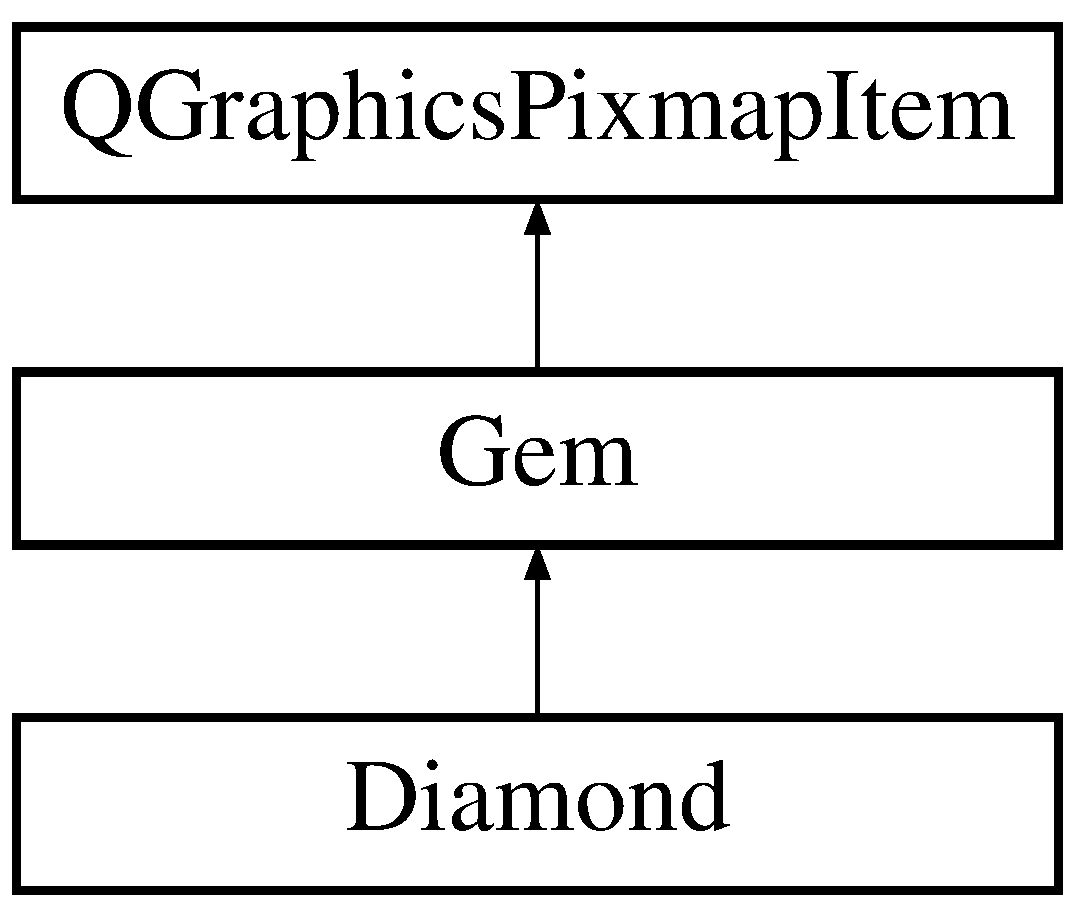
\includegraphics[height=3.000000cm]{classGem}
\end{center}
\end{figure}
\subsection*{Public Member Functions}
\begin{DoxyCompactItemize}
\item 
virtual void \hyperlink{classGem_a7b8029d12d3bfd6d2c897f5c0f930c38}{draw\-Gem} (Q\-Graphics\-Scene $\ast$scene\-\_\-input)
\begin{DoxyCompactList}\small\item\em Draws the \hyperlink{classGem}{Gem} on the scene. \end{DoxyCompactList}\item 
int \hyperlink{classGem_a455e97a96da9442751f6ef221712c031}{get\-Point\-Value} ()
\begin{DoxyCompactList}\small\item\em Get the score given to the player on capture of the \hyperlink{classGem}{Gem}. \end{DoxyCompactList}\item 
bool \hyperlink{classGem_ab7735a029b7980d8851f290c0b8c444f}{get\-Removed\-From\-Screen} ()
\begin{DoxyCompactList}\small\item\em Get if player is not on the screen in the client. \end{DoxyCompactList}\item 
void \hyperlink{classGem_a918dd824b208662f8f215cd961638c46}{set\-Removed\-From\-Screen} (bool input)
\begin{DoxyCompactList}\small\item\em Set whether the \hyperlink{classGem}{Gem} is not on the screen in the client. \end{DoxyCompactList}\item 
bool \hyperlink{classGem_a2507142f69f0c99408a0ce779994db9e}{get\-Is\-On\-Screen} ()
\begin{DoxyCompactList}\small\item\em Get if the \hyperlink{classGem}{Gem} is on the screen in the server. \end{DoxyCompactList}\item 
void \hyperlink{classGem_a65b10ba218d11d69dca0477408dc4da8}{set\-Is\-On\-Screen} (bool input)
\begin{DoxyCompactList}\small\item\em Set whether the \hyperlink{classGem}{Gem} is in the screen in the server. \end{DoxyCompactList}\item 
void \hyperlink{classGem_a791395b9a42eb3a55eb7791621de46e0}{set\-Point\-Value} (int input)
\begin{DoxyCompactList}\small\item\em Set the number of points a player capturing the \hyperlink{classGem}{Gem} would receive. \end{DoxyCompactList}\item 
void \hyperlink{classGem_a05d61a981b55959477159f0dc029b77a}{remove} (Q\-Graphics\-Scene $\ast$input\-\_\-scene)
\begin{DoxyCompactList}\small\item\em Removes the \hyperlink{classGem}{Gem} from the scene. \end{DoxyCompactList}\end{DoxyCompactItemize}


\subsection{Detailed Description}
Describes a \hyperlink{classGem}{Gem} Describes a \hyperlink{classGem}{Gem}, an object that can be captured by players to earn points. Handles the drawing, placement, update, and score of the gems. 

\subsection{Member Function Documentation}
\hypertarget{classGem_a7b8029d12d3bfd6d2c897f5c0f930c38}{\index{Gem@{Gem}!draw\-Gem@{draw\-Gem}}
\index{draw\-Gem@{draw\-Gem}!Gem@{Gem}}
\subsubsection[{draw\-Gem}]{\setlength{\rightskip}{0pt plus 5cm}virtual void Gem\-::draw\-Gem (
\begin{DoxyParamCaption}
\item[{Q\-Graphics\-Scene $\ast$}]{scene\-\_\-input}
\end{DoxyParamCaption}
)\hspace{0.3cm}{\ttfamily [inline]}, {\ttfamily [virtual]}}}\label{classGem_a7b8029d12d3bfd6d2c897f5c0f930c38}


Draws the \hyperlink{classGem}{Gem} on the scene. 


\begin{DoxyParams}{Parameters}
{\em scene\-\_\-input} & the scene on which the \hyperlink{classGem}{Gem} is drawn \\
\hline
\end{DoxyParams}


Reimplemented in \hyperlink{classDiamond_a7139292b0be9a93f99f48e6c00fac072}{Diamond}.

\hypertarget{classGem_a2507142f69f0c99408a0ce779994db9e}{\index{Gem@{Gem}!get\-Is\-On\-Screen@{get\-Is\-On\-Screen}}
\index{get\-Is\-On\-Screen@{get\-Is\-On\-Screen}!Gem@{Gem}}
\subsubsection[{get\-Is\-On\-Screen}]{\setlength{\rightskip}{0pt plus 5cm}bool Gem\-::get\-Is\-On\-Screen (
\begin{DoxyParamCaption}
{}
\end{DoxyParamCaption}
)}}\label{classGem_a2507142f69f0c99408a0ce779994db9e}


Get if the \hyperlink{classGem}{Gem} is on the screen in the server. 

\begin{DoxyReturn}{Returns}
true, if yes, false, if not 
\end{DoxyReturn}
\hypertarget{classGem_a455e97a96da9442751f6ef221712c031}{\index{Gem@{Gem}!get\-Point\-Value@{get\-Point\-Value}}
\index{get\-Point\-Value@{get\-Point\-Value}!Gem@{Gem}}
\subsubsection[{get\-Point\-Value}]{\setlength{\rightskip}{0pt plus 5cm}int Gem\-::get\-Point\-Value (
\begin{DoxyParamCaption}
{}
\end{DoxyParamCaption}
)}}\label{classGem_a455e97a96da9442751f6ef221712c031}


Get the score given to the player on capture of the \hyperlink{classGem}{Gem}. 

\begin{DoxyReturn}{Returns}
the value of the score 
\end{DoxyReturn}
\hypertarget{classGem_ab7735a029b7980d8851f290c0b8c444f}{\index{Gem@{Gem}!get\-Removed\-From\-Screen@{get\-Removed\-From\-Screen}}
\index{get\-Removed\-From\-Screen@{get\-Removed\-From\-Screen}!Gem@{Gem}}
\subsubsection[{get\-Removed\-From\-Screen}]{\setlength{\rightskip}{0pt plus 5cm}bool Gem\-::get\-Removed\-From\-Screen (
\begin{DoxyParamCaption}
{}
\end{DoxyParamCaption}
)}}\label{classGem_ab7735a029b7980d8851f290c0b8c444f}


Get if player is not on the screen in the client. 

\begin{DoxyReturn}{Returns}
true, if not on the screen, false, otherwise 
\end{DoxyReturn}
\hypertarget{classGem_a05d61a981b55959477159f0dc029b77a}{\index{Gem@{Gem}!remove@{remove}}
\index{remove@{remove}!Gem@{Gem}}
\subsubsection[{remove}]{\setlength{\rightskip}{0pt plus 5cm}void Gem\-::remove (
\begin{DoxyParamCaption}
\item[{Q\-Graphics\-Scene $\ast$}]{input\-\_\-scene}
\end{DoxyParamCaption}
)}}\label{classGem_a05d61a981b55959477159f0dc029b77a}


Removes the \hyperlink{classGem}{Gem} from the scene. 


\begin{DoxyParams}{Parameters}
{\em input\-\_\-scene} & the scene from which the \hyperlink{classGem}{Gem} is to be removed \\
\hline
\end{DoxyParams}
\hypertarget{classGem_a65b10ba218d11d69dca0477408dc4da8}{\index{Gem@{Gem}!set\-Is\-On\-Screen@{set\-Is\-On\-Screen}}
\index{set\-Is\-On\-Screen@{set\-Is\-On\-Screen}!Gem@{Gem}}
\subsubsection[{set\-Is\-On\-Screen}]{\setlength{\rightskip}{0pt plus 5cm}void Gem\-::set\-Is\-On\-Screen (
\begin{DoxyParamCaption}
\item[{bool}]{input}
\end{DoxyParamCaption}
)}}\label{classGem_a65b10ba218d11d69dca0477408dc4da8}


Set whether the \hyperlink{classGem}{Gem} is in the screen in the server. 


\begin{DoxyParams}{Parameters}
{\em input} & the value to set \\
\hline
\end{DoxyParams}
\hypertarget{classGem_a791395b9a42eb3a55eb7791621de46e0}{\index{Gem@{Gem}!set\-Point\-Value@{set\-Point\-Value}}
\index{set\-Point\-Value@{set\-Point\-Value}!Gem@{Gem}}
\subsubsection[{set\-Point\-Value}]{\setlength{\rightskip}{0pt plus 5cm}void Gem\-::set\-Point\-Value (
\begin{DoxyParamCaption}
\item[{int}]{input}
\end{DoxyParamCaption}
)}}\label{classGem_a791395b9a42eb3a55eb7791621de46e0}


Set the number of points a player capturing the \hyperlink{classGem}{Gem} would receive. 


\begin{DoxyParams}{Parameters}
{\em input} & the value of the number of points \\
\hline
\end{DoxyParams}
\hypertarget{classGem_a918dd824b208662f8f215cd961638c46}{\index{Gem@{Gem}!set\-Removed\-From\-Screen@{set\-Removed\-From\-Screen}}
\index{set\-Removed\-From\-Screen@{set\-Removed\-From\-Screen}!Gem@{Gem}}
\subsubsection[{set\-Removed\-From\-Screen}]{\setlength{\rightskip}{0pt plus 5cm}void Gem\-::set\-Removed\-From\-Screen (
\begin{DoxyParamCaption}
\item[{bool}]{input}
\end{DoxyParamCaption}
)}}\label{classGem_a918dd824b208662f8f215cd961638c46}


Set whether the \hyperlink{classGem}{Gem} is not on the screen in the client. 


\begin{DoxyParams}{Parameters}
{\em input} & the value to set \\
\hline
\end{DoxyParams}


The documentation for this class was generated from the following file\-:\begin{DoxyCompactItemize}
\item 
gem.\-h\end{DoxyCompactItemize}

\hypertarget{classGraphicsComponent}{\section{Graphics\-Component Class Reference}
\label{classGraphicsComponent}\index{Graphics\-Component@{Graphics\-Component}}
}


Component of a \hyperlink{classGameObject}{Game\-Object} that handles the graphics Handles how to display a game object, and updating the display based on the \hyperlink{classState}{State}.  




{\ttfamily \#include $<$graphicscomponent.\-h$>$}

Inheritance diagram for Graphics\-Component\-:\begin{figure}[H]
\begin{center}
\leavevmode
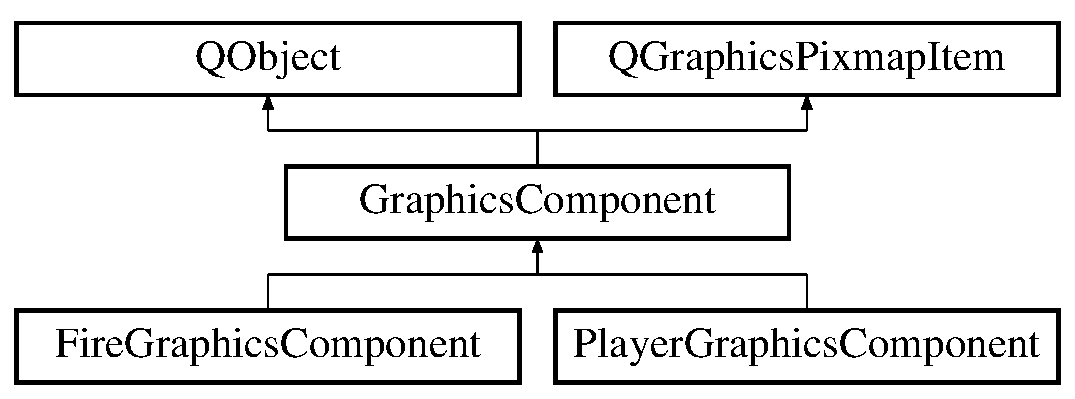
\includegraphics[height=3.000000cm]{classGraphicsComponent}
\end{center}
\end{figure}
\subsection*{Public Member Functions}
\begin{DoxyCompactItemize}
\item 
\hypertarget{classGraphicsComponent_a67fc1b715989a5e18d32e26b27a55c50}{\hyperlink{classGraphicsComponent_a67fc1b715989a5e18d32e26b27a55c50}{Graphics\-Component} ()}\label{classGraphicsComponent_a67fc1b715989a5e18d32e26b27a55c50}

\begin{DoxyCompactList}\small\item\em Constructor. \end{DoxyCompactList}\item 
\hypertarget{classGraphicsComponent_abdd6b7255c198efc5ae2817099760293}{\hyperlink{classGraphicsComponent_abdd6b7255c198efc5ae2817099760293}{$\sim$\-Graphics\-Component} ()}\label{classGraphicsComponent_abdd6b7255c198efc5ae2817099760293}

\begin{DoxyCompactList}\small\item\em Destructor. \end{DoxyCompactList}\item 
virtual void \hyperlink{classGraphicsComponent_a744134b79cf11b2ff29fb7802923fda9}{update} (\hyperlink{classGameObject}{Game\-Object} \&game\-Object)
\begin{DoxyCompactList}\small\item\em Updates the graphics of the game\-Object. \end{DoxyCompactList}\item 
bool \hyperlink{classGraphicsComponent_ab670b9ae59d04b87f2602332997ea059}{get\-Is\-Dangerous} ()
\begin{DoxyCompactList}\small\item\em Get whether the \hyperlink{classGameObject}{Game\-Object} corresponding to the \hyperlink{classGraphicsComponent}{Graphics\-Component} is dangerous. \end{DoxyCompactList}\item 
virtual std\-::vector$<$ qreal $>$ \hyperlink{classGraphicsComponent_a653e0474dd66fc1876f405831e121631}{get\-Size\-Position\-Of\-Object} ()=0
\begin{DoxyCompactList}\small\item\em Get the size and position. \end{DoxyCompactList}\end{DoxyCompactItemize}
\subsection*{Protected Attributes}
\begin{DoxyCompactItemize}
\item 
\hypertarget{classGraphicsComponent_adbd0c2b6656a50c654231f1861e2e6ed}{bool \hyperlink{classGraphicsComponent_adbd0c2b6656a50c654231f1861e2e6ed}{is\-Dangerous}}\label{classGraphicsComponent_adbd0c2b6656a50c654231f1861e2e6ed}

\begin{DoxyCompactList}\small\item\em Specifies whether a player will be destroyed by the \hyperlink{classGameObject}{Game\-Object} corresponding to the \hyperlink{classGraphicsComponent}{Graphics\-Component}. \end{DoxyCompactList}\end{DoxyCompactItemize}


\subsection{Detailed Description}
Component of a \hyperlink{classGameObject}{Game\-Object} that handles the graphics Handles how to display a game object, and updating the display based on the \hyperlink{classState}{State}. 

\subsection{Member Function Documentation}
\hypertarget{classGraphicsComponent_ab670b9ae59d04b87f2602332997ea059}{\index{Graphics\-Component@{Graphics\-Component}!get\-Is\-Dangerous@{get\-Is\-Dangerous}}
\index{get\-Is\-Dangerous@{get\-Is\-Dangerous}!GraphicsComponent@{Graphics\-Component}}
\subsubsection[{get\-Is\-Dangerous}]{\setlength{\rightskip}{0pt plus 5cm}bool Graphics\-Component\-::get\-Is\-Dangerous (
\begin{DoxyParamCaption}
{}
\end{DoxyParamCaption}
)}}\label{classGraphicsComponent_ab670b9ae59d04b87f2602332997ea059}


Get whether the \hyperlink{classGameObject}{Game\-Object} corresponding to the \hyperlink{classGraphicsComponent}{Graphics\-Component} is dangerous. 

\begin{DoxyReturn}{Returns}
true, if a player will be destroyed by it, false, otherwise 
\end{DoxyReturn}
\hypertarget{classGraphicsComponent_a653e0474dd66fc1876f405831e121631}{\index{Graphics\-Component@{Graphics\-Component}!get\-Size\-Position\-Of\-Object@{get\-Size\-Position\-Of\-Object}}
\index{get\-Size\-Position\-Of\-Object@{get\-Size\-Position\-Of\-Object}!GraphicsComponent@{Graphics\-Component}}
\subsubsection[{get\-Size\-Position\-Of\-Object}]{\setlength{\rightskip}{0pt plus 5cm}virtual std\-::vector$<$qreal$>$ Graphics\-Component\-::get\-Size\-Position\-Of\-Object (
\begin{DoxyParamCaption}
{}
\end{DoxyParamCaption}
)\hspace{0.3cm}{\ttfamily [pure virtual]}}}\label{classGraphicsComponent_a653e0474dd66fc1876f405831e121631}


Get the size and position. 

\begin{DoxyReturn}{Returns}
a vector of type qreal, with width, height, x coordinate, y coordinate filled in that order 
\end{DoxyReturn}


Implemented in \hyperlink{classPlayerGraphicsComponent_a9e4f6d92f14886b23791ac2eb8846349}{Player\-Graphics\-Component}, and \hyperlink{classFireGraphicsComponent_a61a1db833ae5aff3a0b4464d3a7d9761}{Fire\-Graphics\-Component}.

\hypertarget{classGraphicsComponent_a744134b79cf11b2ff29fb7802923fda9}{\index{Graphics\-Component@{Graphics\-Component}!update@{update}}
\index{update@{update}!GraphicsComponent@{Graphics\-Component}}
\subsubsection[{update}]{\setlength{\rightskip}{0pt plus 5cm}virtual void Graphics\-Component\-::update (
\begin{DoxyParamCaption}
\item[{{\bf Game\-Object} \&}]{game\-Object}
\end{DoxyParamCaption}
)\hspace{0.3cm}{\ttfamily [inline]}, {\ttfamily [virtual]}}}\label{classGraphicsComponent_a744134b79cf11b2ff29fb7802923fda9}


Updates the graphics of the game\-Object. 


\begin{DoxyParams}{Parameters}
{\em game\-Object} & the \hyperlink{classGameObject}{Game\-Object} the \hyperlink{classGraphicsComponent}{Graphics\-Component} belongs to \\
\hline
\end{DoxyParams}


Reimplemented in \hyperlink{classPlayerGraphicsComponent_ace3901cc8345392c22315f24d617e98b}{Player\-Graphics\-Component}, and \hyperlink{classFireGraphicsComponent_a241b7300febe73c29791803784d65c4a}{Fire\-Graphics\-Component}.



The documentation for this class was generated from the following file\-:\begin{DoxyCompactItemize}
\item 
graphicscomponent.\-h\end{DoxyCompactItemize}

\hypertarget{classHumanInputComponent}{\section{Human\-Input\-Component Class Reference}
\label{classHumanInputComponent}\index{Human\-Input\-Component@{Human\-Input\-Component}}
}


Component of \hyperlink{classGameObject}{Game\-Object} that handles human input Handles keyboard input (key press and key release) events and updates the \hyperlink{classState}{State} of the \hyperlink{classGameObject}{Game\-Object}.  




{\ttfamily \#include $<$humaninputcomponent.\-h$>$}

Inheritance diagram for Human\-Input\-Component\-:\begin{figure}[H]
\begin{center}
\leavevmode
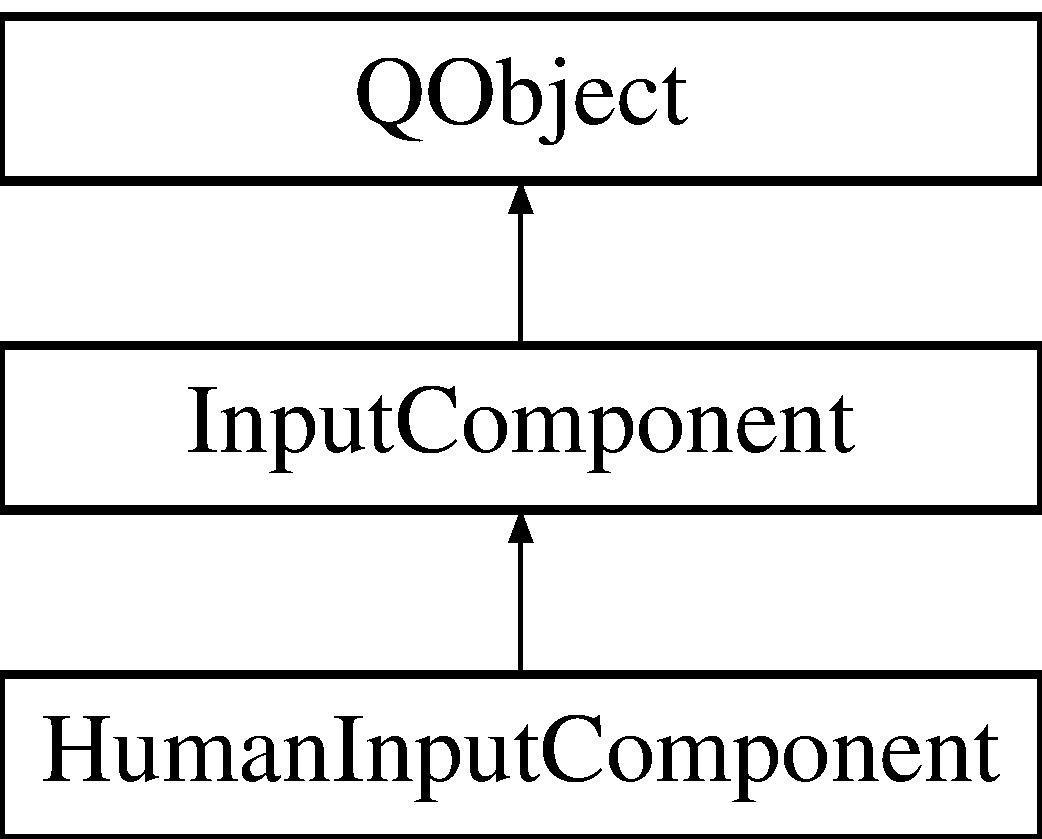
\includegraphics[height=3.000000cm]{classHumanInputComponent}
\end{center}
\end{figure}
\subsection*{Public Member Functions}
\begin{DoxyCompactItemize}
\item 
\hyperlink{classHumanInputComponent_af8c2bd301c382eb5f353089010b20519}{Human\-Input\-Component} (\hyperlink{classKeys}{Keys} $\ast$\hyperlink{classInputComponent_ab4ab656db9378e27c34ff39d1e790308}{keys})
\begin{DoxyCompactList}\small\item\em Constructor. \end{DoxyCompactList}\item 
\hypertarget{classHumanInputComponent_acb45d35e71bd98d382d3684a88aaf42e}{virtual \hyperlink{classHumanInputComponent_acb45d35e71bd98d382d3684a88aaf42e}{$\sim$\-Human\-Input\-Component} ()}\label{classHumanInputComponent_acb45d35e71bd98d382d3684a88aaf42e}

\begin{DoxyCompactList}\small\item\em Destructor. \end{DoxyCompactList}\item 
virtual void \hyperlink{classHumanInputComponent_a10e31c29b86c3c6fff99e699dca28e82}{update} (\hyperlink{classGameObject}{Game\-Object} \&game\-Object)
\begin{DoxyCompactList}\small\item\em Updates the \hyperlink{classInputComponent}{Input\-Component} of game\-Object. \end{DoxyCompactList}\item 
bool \hyperlink{classHumanInputComponent_ac06da10a796d7975c1a97c2618e8fcfd}{event} (Q\-Event $\ast$event)
\begin{DoxyCompactList}\small\item\em Received keyboard events and updates accordingly. \end{DoxyCompactList}\item 
virtual bool \hyperlink{classHumanInputComponent_ac6701b0da2dea7c3764d9159625f269f}{accepts\-Input} ()
\begin{DoxyCompactList}\small\item\em Get whether the corresponding \hyperlink{classGameObject}{Game\-Object} accepts input from th keyboard. \end{DoxyCompactList}\end{DoxyCompactItemize}
\subsection*{Additional Inherited Members}


\subsection{Detailed Description}
Component of \hyperlink{classGameObject}{Game\-Object} that handles human input Handles keyboard input (key press and key release) events and updates the \hyperlink{classState}{State} of the \hyperlink{classGameObject}{Game\-Object}. 

\subsection{Constructor \& Destructor Documentation}
\hypertarget{classHumanInputComponent_af8c2bd301c382eb5f353089010b20519}{\index{Human\-Input\-Component@{Human\-Input\-Component}!Human\-Input\-Component@{Human\-Input\-Component}}
\index{Human\-Input\-Component@{Human\-Input\-Component}!HumanInputComponent@{Human\-Input\-Component}}
\subsubsection[{Human\-Input\-Component}]{\setlength{\rightskip}{0pt plus 5cm}Human\-Input\-Component\-::\-Human\-Input\-Component (
\begin{DoxyParamCaption}
\item[{{\bf Keys} $\ast$}]{keys}
\end{DoxyParamCaption}
)}}\label{classHumanInputComponent_af8c2bd301c382eb5f353089010b20519}


Constructor. 


\begin{DoxyParams}{Parameters}
{\em keys} & Specify the keys for jump, left, and right \\
\hline
\end{DoxyParams}


\subsection{Member Function Documentation}
\hypertarget{classHumanInputComponent_ac6701b0da2dea7c3764d9159625f269f}{\index{Human\-Input\-Component@{Human\-Input\-Component}!accepts\-Input@{accepts\-Input}}
\index{accepts\-Input@{accepts\-Input}!HumanInputComponent@{Human\-Input\-Component}}
\subsubsection[{accepts\-Input}]{\setlength{\rightskip}{0pt plus 5cm}virtual bool Human\-Input\-Component\-::accepts\-Input (
\begin{DoxyParamCaption}
{}
\end{DoxyParamCaption}
)\hspace{0.3cm}{\ttfamily [virtual]}}}\label{classHumanInputComponent_ac6701b0da2dea7c3764d9159625f269f}


Get whether the corresponding \hyperlink{classGameObject}{Game\-Object} accepts input from th keyboard. 

\begin{DoxyReturn}{Returns}
true, as \hyperlink{classGameObject}{Game\-Object} with \hyperlink{classHumanInputComponent}{Human\-Input\-Component} accepts input 
\end{DoxyReturn}


Implements \hyperlink{classInputComponent_a27a4de99780ddf7d7a4f9d469f13640c}{Input\-Component}.

\hypertarget{classHumanInputComponent_ac06da10a796d7975c1a97c2618e8fcfd}{\index{Human\-Input\-Component@{Human\-Input\-Component}!event@{event}}
\index{event@{event}!HumanInputComponent@{Human\-Input\-Component}}
\subsubsection[{event}]{\setlength{\rightskip}{0pt plus 5cm}bool Human\-Input\-Component\-::event (
\begin{DoxyParamCaption}
\item[{Q\-Event $\ast$}]{event}
\end{DoxyParamCaption}
)\hspace{0.3cm}{\ttfamily [virtual]}}}\label{classHumanInputComponent_ac06da10a796d7975c1a97c2618e8fcfd}


Received keyboard events and updates accordingly. 


\begin{DoxyParams}{Parameters}
{\em event} & the event received \\
\hline
\end{DoxyParams}
\begin{DoxyReturn}{Returns}
true, if event is recognized and \hyperlink{classState}{State} updated, false, otherwise 
\end{DoxyReturn}


Reimplemented from \hyperlink{classInputComponent_a6e9e903cdb89d7eb7d9ab89d1734f7aa}{Input\-Component}.

\hypertarget{classHumanInputComponent_a10e31c29b86c3c6fff99e699dca28e82}{\index{Human\-Input\-Component@{Human\-Input\-Component}!update@{update}}
\index{update@{update}!HumanInputComponent@{Human\-Input\-Component}}
\subsubsection[{update}]{\setlength{\rightskip}{0pt plus 5cm}virtual void Human\-Input\-Component\-::update (
\begin{DoxyParamCaption}
\item[{{\bf Game\-Object} \&}]{game\-Object}
\end{DoxyParamCaption}
)\hspace{0.3cm}{\ttfamily [virtual]}}}\label{classHumanInputComponent_a10e31c29b86c3c6fff99e699dca28e82}


Updates the \hyperlink{classInputComponent}{Input\-Component} of game\-Object. 


\begin{DoxyParams}{Parameters}
{\em game\-Object} & the game\-Object to be updated \\
\hline
\end{DoxyParams}


Implements \hyperlink{classInputComponent_a93e790f7279e842ee249fefe7dbf7b32}{Input\-Component}.



The documentation for this class was generated from the following file\-:\begin{DoxyCompactItemize}
\item 
humaninputcomponent.\-h\end{DoxyCompactItemize}

\hypertarget{classInputComponent}{\section{Input\-Component Class Reference}
\label{classInputComponent}\index{Input\-Component@{Input\-Component}}
}


Component to handle inputs given to the \hyperlink{classGameObject}{Game\-Object} Handles the accepting of inputs, processes it, and updates the \hyperlink{classState}{State} of the \hyperlink{classGameObject}{Game\-Object} accordingly.  




{\ttfamily \#include $<$inputcomponent.\-h$>$}

Inheritance diagram for Input\-Component\-:\begin{figure}[H]
\begin{center}
\leavevmode
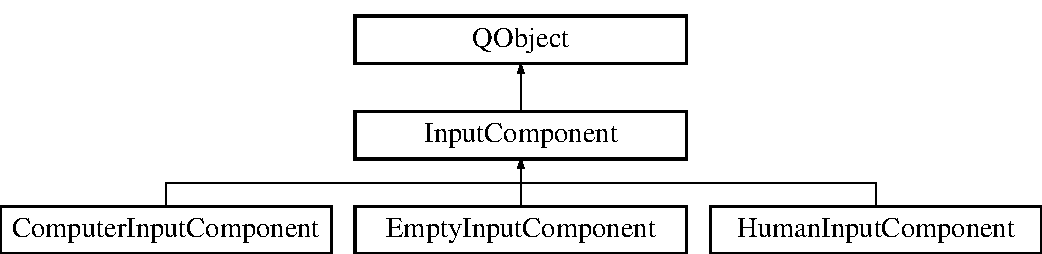
\includegraphics[height=3.000000cm]{classInputComponent}
\end{center}
\end{figure}
\subsection*{Public Member Functions}
\begin{DoxyCompactItemize}
\item 
\hypertarget{classInputComponent_ae3af150f66c8e72ea4bef4b089c48d99}{\hyperlink{classInputComponent_ae3af150f66c8e72ea4bef4b089c48d99}{Input\-Component} ()}\label{classInputComponent_ae3af150f66c8e72ea4bef4b089c48d99}

\begin{DoxyCompactList}\small\item\em Constructor. \end{DoxyCompactList}\item 
\hypertarget{classInputComponent_a2004af6e68e0206f045518cb6ee43981}{virtual \hyperlink{classInputComponent_a2004af6e68e0206f045518cb6ee43981}{$\sim$\-Input\-Component} ()}\label{classInputComponent_a2004af6e68e0206f045518cb6ee43981}

\begin{DoxyCompactList}\small\item\em Destructor. \end{DoxyCompactList}\item 
virtual void \hyperlink{classInputComponent_a93e790f7279e842ee249fefe7dbf7b32}{update} (\hyperlink{classGameObject}{Game\-Object} \&game\-Object)=0
\begin{DoxyCompactList}\small\item\em Updates the \hyperlink{classState}{State} of game\-Object. \end{DoxyCompactList}\item 
virtual bool \hyperlink{classInputComponent_a6e9e903cdb89d7eb7d9ab89d1734f7aa}{event} (Q\-Event $\ast$event)
\begin{DoxyCompactList}\small\item\em Receives events, processes it, and calls update accordingly. \end{DoxyCompactList}\item 
virtual bool \hyperlink{classInputComponent_a27a4de99780ddf7d7a4f9d469f13640c}{accepts\-Input} ()=0
\begin{DoxyCompactList}\small\item\em Get whether the corresponding \hyperlink{classGameObject}{Game\-Object} accepts input from the keyboard. \end{DoxyCompactList}\end{DoxyCompactItemize}
\subsection*{Public Attributes}
\begin{DoxyCompactItemize}
\item 
\hypertarget{classInputComponent_ab4ab656db9378e27c34ff39d1e790308}{\hyperlink{classKeys}{Keys} $\ast$ \hyperlink{classInputComponent_ab4ab656db9378e27c34ff39d1e790308}{keys}}\label{classInputComponent_ab4ab656db9378e27c34ff39d1e790308}

\begin{DoxyCompactList}\small\item\em Stores the keys corresponding to the motion of the \hyperlink{classGameObject}{Game\-Object}. \end{DoxyCompactList}\end{DoxyCompactItemize}


\subsection{Detailed Description}
Component to handle inputs given to the \hyperlink{classGameObject}{Game\-Object} Handles the accepting of inputs, processes it, and updates the \hyperlink{classState}{State} of the \hyperlink{classGameObject}{Game\-Object} accordingly. 

\subsection{Member Function Documentation}
\hypertarget{classInputComponent_a27a4de99780ddf7d7a4f9d469f13640c}{\index{Input\-Component@{Input\-Component}!accepts\-Input@{accepts\-Input}}
\index{accepts\-Input@{accepts\-Input}!InputComponent@{Input\-Component}}
\subsubsection[{accepts\-Input}]{\setlength{\rightskip}{0pt plus 5cm}virtual bool Input\-Component\-::accepts\-Input (
\begin{DoxyParamCaption}
{}
\end{DoxyParamCaption}
)\hspace{0.3cm}{\ttfamily [pure virtual]}}}\label{classInputComponent_a27a4de99780ddf7d7a4f9d469f13640c}


Get whether the corresponding \hyperlink{classGameObject}{Game\-Object} accepts input from the keyboard. 

\begin{DoxyReturn}{Returns}
true, if yes, false, otherwise 
\end{DoxyReturn}


Implemented in \hyperlink{classHumanInputComponent_ac6701b0da2dea7c3764d9159625f269f}{Human\-Input\-Component}, \hyperlink{classComputerInputComponent_a20fda9adf00a1be24b9bcca0b8662a35}{Computer\-Input\-Component}, and \hyperlink{classEmptyInputComponent_a821f567bd824806e2322f22ce5955b06}{Empty\-Input\-Component}.

\hypertarget{classInputComponent_a6e9e903cdb89d7eb7d9ab89d1734f7aa}{\index{Input\-Component@{Input\-Component}!event@{event}}
\index{event@{event}!InputComponent@{Input\-Component}}
\subsubsection[{event}]{\setlength{\rightskip}{0pt plus 5cm}virtual bool Input\-Component\-::event (
\begin{DoxyParamCaption}
\item[{Q\-Event $\ast$}]{event}
\end{DoxyParamCaption}
)\hspace{0.3cm}{\ttfamily [virtual]}}}\label{classInputComponent_a6e9e903cdb89d7eb7d9ab89d1734f7aa}


Receives events, processes it, and calls update accordingly. 


\begin{DoxyParams}{Parameters}
{\em event} & the event received \\
\hline
\end{DoxyParams}
\begin{DoxyReturn}{Returns}
true, if the event is recogized and processed, false, otherwise 
\end{DoxyReturn}


Reimplemented in \hyperlink{classHumanInputComponent_ac06da10a796d7975c1a97c2618e8fcfd}{Human\-Input\-Component}.

\hypertarget{classInputComponent_a93e790f7279e842ee249fefe7dbf7b32}{\index{Input\-Component@{Input\-Component}!update@{update}}
\index{update@{update}!InputComponent@{Input\-Component}}
\subsubsection[{update}]{\setlength{\rightskip}{0pt plus 5cm}virtual void Input\-Component\-::update (
\begin{DoxyParamCaption}
\item[{{\bf Game\-Object} \&}]{game\-Object}
\end{DoxyParamCaption}
)\hspace{0.3cm}{\ttfamily [pure virtual]}}}\label{classInputComponent_a93e790f7279e842ee249fefe7dbf7b32}


Updates the \hyperlink{classState}{State} of game\-Object. 


\begin{DoxyParams}{Parameters}
{\em game\-Object} & the \hyperlink{classGameObject}{Game\-Object} to be updated \\
\hline
\end{DoxyParams}


Implemented in \hyperlink{classHumanInputComponent_a10e31c29b86c3c6fff99e699dca28e82}{Human\-Input\-Component}, \hyperlink{classComputerInputComponent_abddd2bdc7efb465f49173a3634148bbc}{Computer\-Input\-Component}, and \hyperlink{classEmptyInputComponent_a5e11b3048e027761e465072cda02a034}{Empty\-Input\-Component}.



The documentation for this class was generated from the following file\-:\begin{DoxyCompactItemize}
\item 
inputcomponent.\-h\end{DoxyCompactItemize}

\hypertarget{classInputHandler}{\section{Input\-Handler Class Reference}
\label{classInputHandler}\index{Input\-Handler@{Input\-Handler}}
}


View that also handles key press and key release events Used to show the scene, and to receive key press and key release events and pass it where needed.  




{\ttfamily \#include $<$inputhandler.\-h$>$}

Inheritance diagram for Input\-Handler\-:\begin{figure}[H]
\begin{center}
\leavevmode
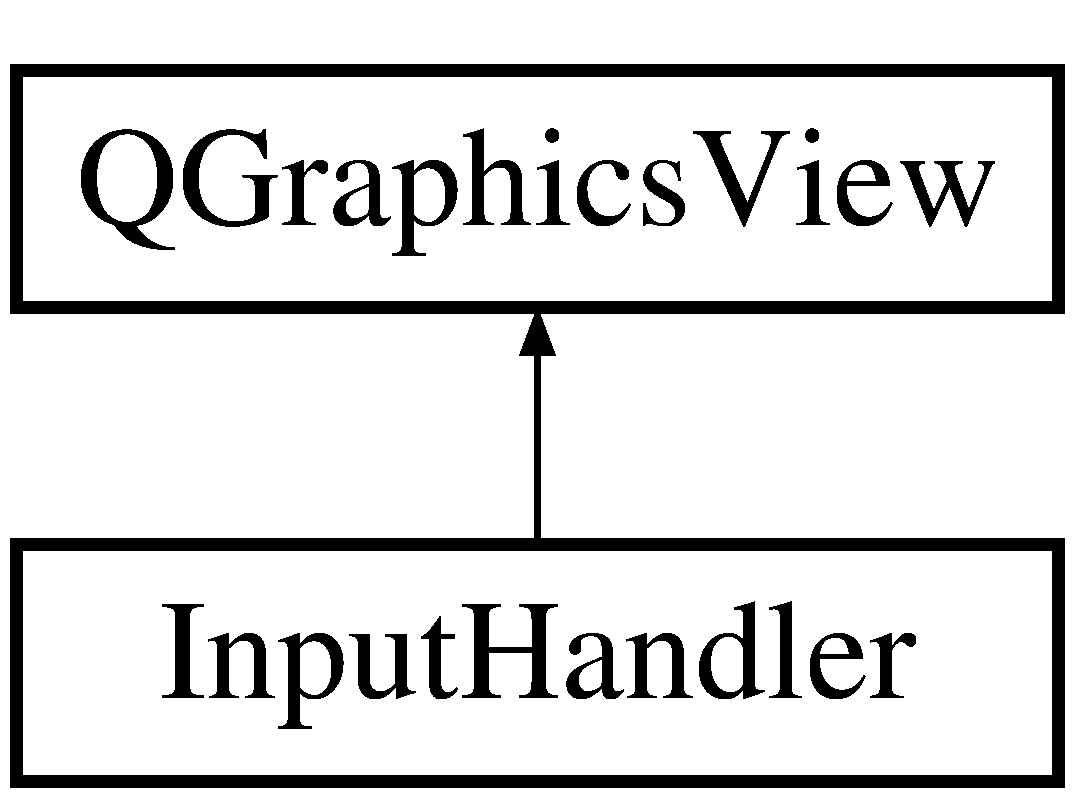
\includegraphics[height=2.000000cm]{classInputHandler}
\end{center}
\end{figure}
\subsection*{Public Member Functions}
\begin{DoxyCompactItemize}
\item 
\hyperlink{classInputHandler_a052ce3adff4a84f49b8380449cf05a5f}{Input\-Handler} (\hyperlink{classGameState}{Game\-State} $\ast$game\-\_\-state)
\begin{DoxyCompactList}\small\item\em Constructor. \end{DoxyCompactList}\item 
void \hyperlink{classInputHandler_a84d1b1ca593d4764114f75c739a8328a}{set\-Game\-Client} (\hyperlink{classClient}{Client} $\ast$client\-\_\-input)
\begin{DoxyCompactList}\small\item\em Store the client object of the game when running in the client. \end{DoxyCompactList}\item 
void \hyperlink{classInputHandler_a30e6f3d86c107f556ff6d904af33a09a}{set\-Game\-State} (\hyperlink{classGameState}{Game\-State} $\ast$game\-\_\-state)
\begin{DoxyCompactList}\small\item\em Set the state of the game here. \end{DoxyCompactList}\item 
void \hyperlink{classInputHandler_a8a3c7799e3930c10da915c7aebd1ae89}{key\-Press\-Event} (Q\-Key\-Event $\ast$event)
\begin{DoxyCompactList}\small\item\em Receive key press events and process it. \end{DoxyCompactList}\item 
void \hyperlink{classInputHandler_a399f396dc428ad1ada35a40170952c55}{key\-Release\-Event} (Q\-Key\-Event $\ast$event)
\begin{DoxyCompactList}\small\item\em Receive key release events and process it. \end{DoxyCompactList}\end{DoxyCompactItemize}


\subsection{Detailed Description}
View that also handles key press and key release events Used to show the scene, and to receive key press and key release events and pass it where needed. 

\subsection{Constructor \& Destructor Documentation}
\hypertarget{classInputHandler_a052ce3adff4a84f49b8380449cf05a5f}{\index{Input\-Handler@{Input\-Handler}!Input\-Handler@{Input\-Handler}}
\index{Input\-Handler@{Input\-Handler}!InputHandler@{Input\-Handler}}
\subsubsection[{Input\-Handler}]{\setlength{\rightskip}{0pt plus 5cm}Input\-Handler\-::\-Input\-Handler (
\begin{DoxyParamCaption}
\item[{{\bf Game\-State} $\ast$}]{game\-\_\-state}
\end{DoxyParamCaption}
)}}\label{classInputHandler_a052ce3adff4a84f49b8380449cf05a5f}


Constructor. 


\begin{DoxyParams}{Parameters}
{\em game\-\_\-state} & the state of the current game \\
\hline
\end{DoxyParams}


\subsection{Member Function Documentation}
\hypertarget{classInputHandler_a8a3c7799e3930c10da915c7aebd1ae89}{\index{Input\-Handler@{Input\-Handler}!key\-Press\-Event@{key\-Press\-Event}}
\index{key\-Press\-Event@{key\-Press\-Event}!InputHandler@{Input\-Handler}}
\subsubsection[{key\-Press\-Event}]{\setlength{\rightskip}{0pt plus 5cm}void Input\-Handler\-::key\-Press\-Event (
\begin{DoxyParamCaption}
\item[{Q\-Key\-Event $\ast$}]{event}
\end{DoxyParamCaption}
)}}\label{classInputHandler_a8a3c7799e3930c10da915c7aebd1ae89}


Receive key press events and process it. 


\begin{DoxyParams}{Parameters}
{\em event} & the key press event received \\
\hline
\end{DoxyParams}
\hypertarget{classInputHandler_a399f396dc428ad1ada35a40170952c55}{\index{Input\-Handler@{Input\-Handler}!key\-Release\-Event@{key\-Release\-Event}}
\index{key\-Release\-Event@{key\-Release\-Event}!InputHandler@{Input\-Handler}}
\subsubsection[{key\-Release\-Event}]{\setlength{\rightskip}{0pt plus 5cm}void Input\-Handler\-::key\-Release\-Event (
\begin{DoxyParamCaption}
\item[{Q\-Key\-Event $\ast$}]{event}
\end{DoxyParamCaption}
)}}\label{classInputHandler_a399f396dc428ad1ada35a40170952c55}


Receive key release events and process it. 


\begin{DoxyParams}{Parameters}
{\em event} & the key release event \\
\hline
\end{DoxyParams}
\hypertarget{classInputHandler_a84d1b1ca593d4764114f75c739a8328a}{\index{Input\-Handler@{Input\-Handler}!set\-Game\-Client@{set\-Game\-Client}}
\index{set\-Game\-Client@{set\-Game\-Client}!InputHandler@{Input\-Handler}}
\subsubsection[{set\-Game\-Client}]{\setlength{\rightskip}{0pt plus 5cm}void Input\-Handler\-::set\-Game\-Client (
\begin{DoxyParamCaption}
\item[{{\bf Client} $\ast$}]{client\-\_\-input}
\end{DoxyParamCaption}
)}}\label{classInputHandler_a84d1b1ca593d4764114f75c739a8328a}


Store the client object of the game when running in the client. 


\begin{DoxyParams}{Parameters}
{\em client\-\_\-input} & \hyperlink{classClient}{Client} object to be stored \\
\hline
\end{DoxyParams}
\hypertarget{classInputHandler_a30e6f3d86c107f556ff6d904af33a09a}{\index{Input\-Handler@{Input\-Handler}!set\-Game\-State@{set\-Game\-State}}
\index{set\-Game\-State@{set\-Game\-State}!InputHandler@{Input\-Handler}}
\subsubsection[{set\-Game\-State}]{\setlength{\rightskip}{0pt plus 5cm}void Input\-Handler\-::set\-Game\-State (
\begin{DoxyParamCaption}
\item[{{\bf Game\-State} $\ast$}]{game\-\_\-state}
\end{DoxyParamCaption}
)}}\label{classInputHandler_a30e6f3d86c107f556ff6d904af33a09a}


Set the state of the game here. 


\begin{DoxyParams}{Parameters}
{\em game\-\_\-state} & the state of the game \\
\hline
\end{DoxyParams}


The documentation for this class was generated from the following file\-:\begin{DoxyCompactItemize}
\item 
inputhandler.\-h\end{DoxyCompactItemize}

\hypertarget{classIsJumping}{\section{Is\-Jumping Class Reference}
\label{classIsJumping}\index{Is\-Jumping@{Is\-Jumping}}
}


\hyperlink{classJumpingState}{Jumping\-State} in which the \hyperlink{classGameObject}{Game\-Object} is jumping.  




{\ttfamily \#include $<$isjumping.\-h$>$}

Inheritance diagram for Is\-Jumping\-:\begin{figure}[H]
\begin{center}
\leavevmode
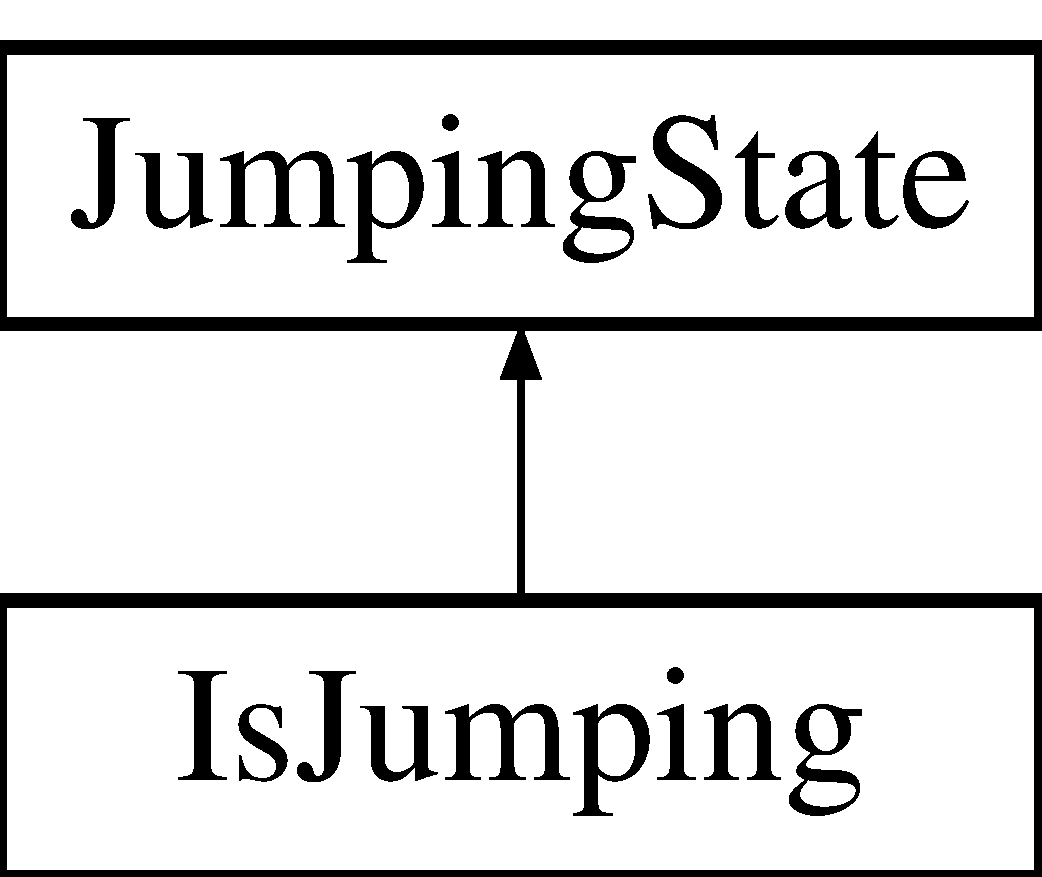
\includegraphics[height=2.000000cm]{classIsJumping}
\end{center}
\end{figure}
\subsection*{Public Member Functions}
\begin{DoxyCompactItemize}
\item 
\hyperlink{classIsJumping_a56fda19df58e162d7cef0db368938a80}{Is\-Jumping} (\hyperlink{classGameObject}{Game\-Object} \&game\-Object)
\begin{DoxyCompactList}\small\item\em Constructor. \end{DoxyCompactList}\item 
\hypertarget{classIsJumping_a6c3eed9fd4ae73c64fee32eaf0c102a0}{virtual \hyperlink{classIsJumping_a6c3eed9fd4ae73c64fee32eaf0c102a0}{$\sim$\-Is\-Jumping} ()}\label{classIsJumping_a6c3eed9fd4ae73c64fee32eaf0c102a0}

\begin{DoxyCompactList}\small\item\em Destructor. \end{DoxyCompactList}\item 
virtual \hyperlink{classJumpingState}{Jumping\-State} $\ast$ \hyperlink{classIsJumping_a3b90719ea42ff820c3e9b26ed7033c4c}{update} (\hyperlink{classInputComponent}{Input\-Component} $\ast$input\-\_\-component, \hyperlink{classGameObject}{Game\-Object} \&game\-\_\-object, std\-::set$<$ Qt\-::\-Key $>$ keys)
\begin{DoxyCompactList}\small\item\em Updates the \hyperlink{classJumpingState}{Jumping\-State}. \end{DoxyCompactList}\item 
virtual \hyperlink{namespaceenumerator_a2f1fb1ef7c57e4549f424d454c1e2179}{enumerator\-::\-Jumping\-State} \hyperlink{classIsJumping_a7cd0858e202392069181097c782710de}{type} ()
\begin{DoxyCompactList}\small\item\em Get the type of the current \hyperlink{classJumpingState}{Jumping\-State}. \end{DoxyCompactList}\end{DoxyCompactItemize}
\subsection*{Additional Inherited Members}


\subsection{Detailed Description}
\hyperlink{classJumpingState}{Jumping\-State} in which the \hyperlink{classGameObject}{Game\-Object} is jumping. 

\subsection{Constructor \& Destructor Documentation}
\hypertarget{classIsJumping_a56fda19df58e162d7cef0db368938a80}{\index{Is\-Jumping@{Is\-Jumping}!Is\-Jumping@{Is\-Jumping}}
\index{Is\-Jumping@{Is\-Jumping}!IsJumping@{Is\-Jumping}}
\subsubsection[{Is\-Jumping}]{\setlength{\rightskip}{0pt plus 5cm}Is\-Jumping\-::\-Is\-Jumping (
\begin{DoxyParamCaption}
\item[{{\bf Game\-Object} \&}]{game\-Object}
\end{DoxyParamCaption}
)}}\label{classIsJumping_a56fda19df58e162d7cef0db368938a80}


Constructor. 


\begin{DoxyParams}{Parameters}
{\em game\-Object} & the \hyperlink{classGameObject}{Game\-Object} the \hyperlink{classJumpingState}{Jumping\-State} belongs \\
\hline
\end{DoxyParams}


\subsection{Member Function Documentation}
\hypertarget{classIsJumping_a7cd0858e202392069181097c782710de}{\index{Is\-Jumping@{Is\-Jumping}!type@{type}}
\index{type@{type}!IsJumping@{Is\-Jumping}}
\subsubsection[{type}]{\setlength{\rightskip}{0pt plus 5cm}virtual {\bf enumerator\-::\-Jumping\-State} Is\-Jumping\-::type (
\begin{DoxyParamCaption}
{}
\end{DoxyParamCaption}
)\hspace{0.3cm}{\ttfamily [virtual]}}}\label{classIsJumping_a7cd0858e202392069181097c782710de}


Get the type of the current \hyperlink{classJumpingState}{Jumping\-State}. 

\begin{DoxyReturn}{Returns}
value of \hyperlink{namespaceenumerator_a2f1fb1ef7c57e4549f424d454c1e2179}{enumerator\-::\-Jumping\-State} with the type 
\end{DoxyReturn}


Implements \hyperlink{classJumpingState_a3c1a2e3c686de946c16e20c717f0a37d}{Jumping\-State}.

\hypertarget{classIsJumping_a3b90719ea42ff820c3e9b26ed7033c4c}{\index{Is\-Jumping@{Is\-Jumping}!update@{update}}
\index{update@{update}!IsJumping@{Is\-Jumping}}
\subsubsection[{update}]{\setlength{\rightskip}{0pt plus 5cm}virtual {\bf Jumping\-State}$\ast$ Is\-Jumping\-::update (
\begin{DoxyParamCaption}
\item[{{\bf Input\-Component} $\ast$}]{input\-\_\-component, }
\item[{{\bf Game\-Object} \&}]{game\-\_\-object, }
\item[{std\-::set$<$ Qt\-::\-Key $>$}]{keys}
\end{DoxyParamCaption}
)\hspace{0.3cm}{\ttfamily [virtual]}}}\label{classIsJumping_a3b90719ea42ff820c3e9b26ed7033c4c}


Updates the \hyperlink{classJumpingState}{Jumping\-State}. 


\begin{DoxyParams}{Parameters}
{\em input\-\_\-component} & the \hyperlink{classInputComponent}{Input\-Component} of the corresponding \hyperlink{classGameObject}{Game\-Object} \\
\hline
{\em game\-\_\-object} & the corresponding \hyperlink{classGameObject}{Game\-Object} \\
\hline
{\em keys} & set of keys currently pressed \\
\hline
\end{DoxyParams}
\begin{DoxyReturn}{Returns}
new \hyperlink{classJumpingState}{Jumping\-State} 
\end{DoxyReturn}


Implements \hyperlink{classJumpingState_a0da4718d614ff36fd1336f01f5ddfa2b}{Jumping\-State}.



The documentation for this class was generated from the following file\-:\begin{DoxyCompactItemize}
\item 
isjumping.\-h\end{DoxyCompactItemize}

\hypertarget{classIsNotJumping}{\section{Is\-Not\-Jumping Class Reference}
\label{classIsNotJumping}\index{Is\-Not\-Jumping@{Is\-Not\-Jumping}}
}


\hyperlink{classJumpingState}{Jumping\-State} in which the \hyperlink{classGameObject}{Game\-Object} is not jumping.  




{\ttfamily \#include $<$isnotjumping.\-h$>$}

Inheritance diagram for Is\-Not\-Jumping\-:\begin{figure}[H]
\begin{center}
\leavevmode
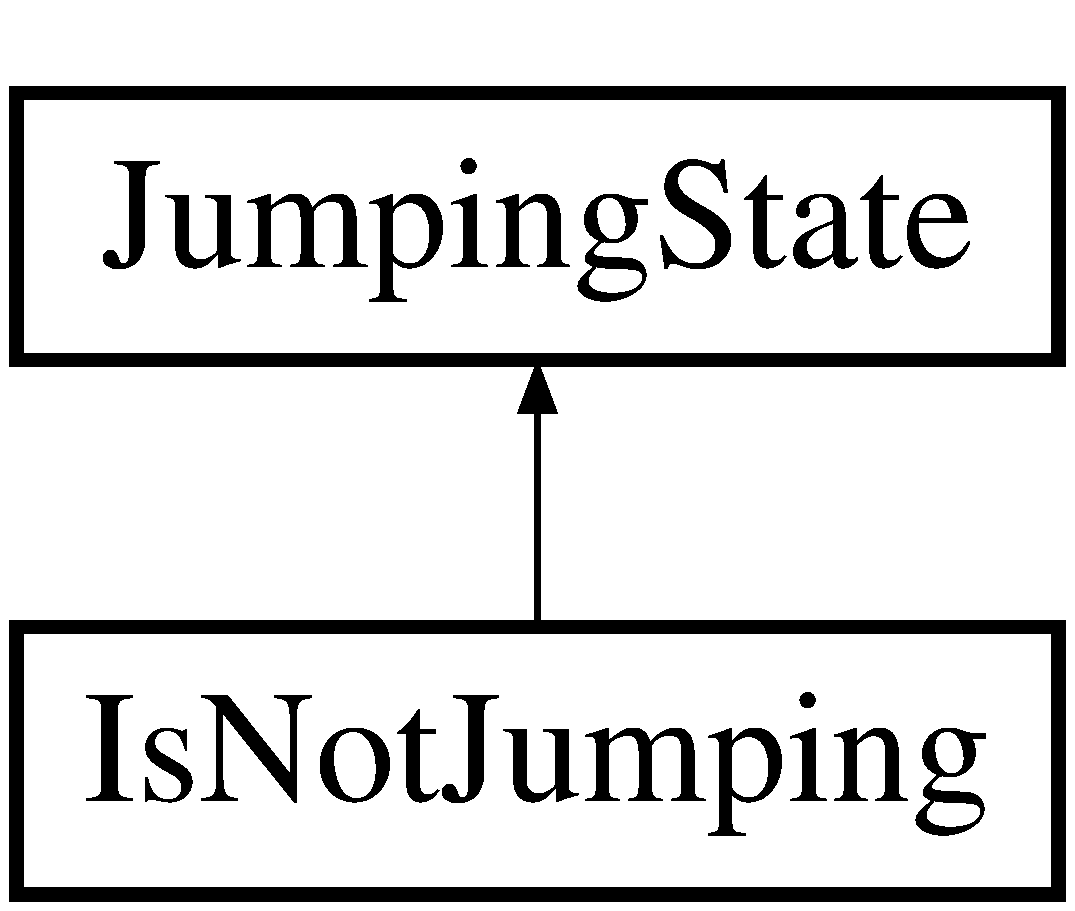
\includegraphics[height=2.000000cm]{classIsNotJumping}
\end{center}
\end{figure}
\subsection*{Public Member Functions}
\begin{DoxyCompactItemize}
\item 
\hyperlink{classIsNotJumping_a4944fdea4979abd38c5cdc7e6eb278ca}{Is\-Not\-Jumping} ()
\begin{DoxyCompactList}\small\item\em Constructor. \end{DoxyCompactList}\item 
\hypertarget{classIsNotJumping_a920891e2d40f4c8b485a857b6830c98c}{virtual \hyperlink{classIsNotJumping_a920891e2d40f4c8b485a857b6830c98c}{$\sim$\-Is\-Not\-Jumping} ()}\label{classIsNotJumping_a920891e2d40f4c8b485a857b6830c98c}

\begin{DoxyCompactList}\small\item\em Destructor. \end{DoxyCompactList}\item 
virtual \hyperlink{classJumpingState}{Jumping\-State} $\ast$ \hyperlink{classIsNotJumping_ae58898ada922fab24c37735bee506c8c}{update} (\hyperlink{classInputComponent}{Input\-Component} $\ast$, \hyperlink{classGameObject}{Game\-Object} \&, std\-::set$<$ Qt\-::\-Key $>$)
\begin{DoxyCompactList}\small\item\em Updates the \hyperlink{classJumpingState}{Jumping\-State}. \end{DoxyCompactList}\item 
virtual \hyperlink{namespaceenumerator_a2f1fb1ef7c57e4549f424d454c1e2179}{enumerator\-::\-Jumping\-State} \hyperlink{classIsNotJumping_a2fc57703b1017b434e82b4a054f2c9d1}{type} ()
\begin{DoxyCompactList}\small\item\em Get the type of the current \hyperlink{classJumpingState}{Jumping\-State}. \end{DoxyCompactList}\end{DoxyCompactItemize}
\subsection*{Additional Inherited Members}


\subsection{Detailed Description}
\hyperlink{classJumpingState}{Jumping\-State} in which the \hyperlink{classGameObject}{Game\-Object} is not jumping. 

\subsection{Constructor \& Destructor Documentation}
\hypertarget{classIsNotJumping_a4944fdea4979abd38c5cdc7e6eb278ca}{\index{Is\-Not\-Jumping@{Is\-Not\-Jumping}!Is\-Not\-Jumping@{Is\-Not\-Jumping}}
\index{Is\-Not\-Jumping@{Is\-Not\-Jumping}!IsNotJumping@{Is\-Not\-Jumping}}
\subsubsection[{Is\-Not\-Jumping}]{\setlength{\rightskip}{0pt plus 5cm}Is\-Not\-Jumping\-::\-Is\-Not\-Jumping (
\begin{DoxyParamCaption}
{}
\end{DoxyParamCaption}
)\hspace{0.3cm}{\ttfamily [inline]}}}\label{classIsNotJumping_a4944fdea4979abd38c5cdc7e6eb278ca}


Constructor. 


\begin{DoxyParams}{Parameters}
{\em game\-Object} & the \hyperlink{classGameObject}{Game\-Object} the \hyperlink{classJumpingState}{Jumping\-State} belongs \\
\hline
\end{DoxyParams}


\subsection{Member Function Documentation}
\hypertarget{classIsNotJumping_a2fc57703b1017b434e82b4a054f2c9d1}{\index{Is\-Not\-Jumping@{Is\-Not\-Jumping}!type@{type}}
\index{type@{type}!IsNotJumping@{Is\-Not\-Jumping}}
\subsubsection[{type}]{\setlength{\rightskip}{0pt plus 5cm}virtual {\bf enumerator\-::\-Jumping\-State} Is\-Not\-Jumping\-::type (
\begin{DoxyParamCaption}
{}
\end{DoxyParamCaption}
)\hspace{0.3cm}{\ttfamily [virtual]}}}\label{classIsNotJumping_a2fc57703b1017b434e82b4a054f2c9d1}


Get the type of the current \hyperlink{classJumpingState}{Jumping\-State}. 

\begin{DoxyReturn}{Returns}
value of \hyperlink{namespaceenumerator_a2f1fb1ef7c57e4549f424d454c1e2179}{enumerator\-::\-Jumping\-State} with the type 
\end{DoxyReturn}


Implements \hyperlink{classJumpingState_a3c1a2e3c686de946c16e20c717f0a37d}{Jumping\-State}.

\hypertarget{classIsNotJumping_ae58898ada922fab24c37735bee506c8c}{\index{Is\-Not\-Jumping@{Is\-Not\-Jumping}!update@{update}}
\index{update@{update}!IsNotJumping@{Is\-Not\-Jumping}}
\subsubsection[{update}]{\setlength{\rightskip}{0pt plus 5cm}virtual {\bf Jumping\-State}$\ast$ Is\-Not\-Jumping\-::update (
\begin{DoxyParamCaption}
\item[{{\bf Input\-Component} $\ast$}]{, }
\item[{{\bf Game\-Object} \&}]{, }
\item[{std\-::set$<$ Qt\-::\-Key $>$}]{}
\end{DoxyParamCaption}
)\hspace{0.3cm}{\ttfamily [virtual]}}}\label{classIsNotJumping_ae58898ada922fab24c37735bee506c8c}


Updates the \hyperlink{classJumpingState}{Jumping\-State}. 


\begin{DoxyParams}{Parameters}
{\em input\-\_\-component} & the \hyperlink{classInputComponent}{Input\-Component} of the corresponding \hyperlink{classGameObject}{Game\-Object} \\
\hline
{\em game\-\_\-object} & the corresponding \hyperlink{classGameObject}{Game\-Object} \\
\hline
{\em keys} & set of keys currently pressed \\
\hline
\end{DoxyParams}
\begin{DoxyReturn}{Returns}
new \hyperlink{classJumpingState}{Jumping\-State} 
\end{DoxyReturn}


Implements \hyperlink{classJumpingState_a0da4718d614ff36fd1336f01f5ddfa2b}{Jumping\-State}.



The documentation for this class was generated from the following file\-:\begin{DoxyCompactItemize}
\item 
isnotjumping.\-h\end{DoxyCompactItemize}

\hypertarget{classJumpingState}{\section{Jumping\-State Class Reference}
\label{classJumpingState}\index{Jumping\-State@{Jumping\-State}}
}


This class is used to store whether the player is jumping or not.  




{\ttfamily \#include $<$jumpingstate.\-h$>$}

Inheritance diagram for Jumping\-State\-:\begin{figure}[H]
\begin{center}
\leavevmode
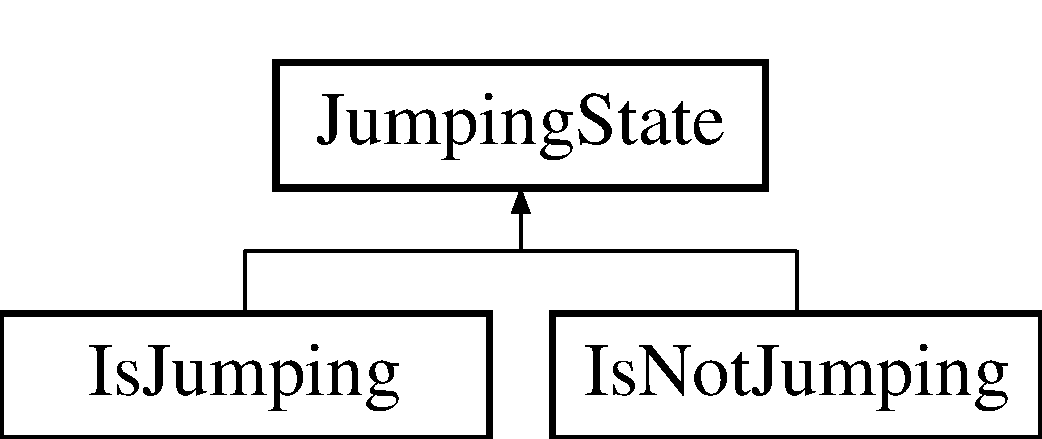
\includegraphics[height=2.000000cm]{classJumpingState}
\end{center}
\end{figure}
\subsection*{Public Member Functions}
\begin{DoxyCompactItemize}
\item 
\hypertarget{classJumpingState_a74a6fbd65de0937c949cb04d7567041f}{\hyperlink{classJumpingState_a74a6fbd65de0937c949cb04d7567041f}{Jumping\-State} ()}\label{classJumpingState_a74a6fbd65de0937c949cb04d7567041f}

\begin{DoxyCompactList}\small\item\em Constructor for Jumping \hyperlink{classState}{State}. \end{DoxyCompactList}\item 
\hypertarget{classJumpingState_aa8fed3f92395e3b1a5c0ab71387fe7da}{virtual \hyperlink{classJumpingState_aa8fed3f92395e3b1a5c0ab71387fe7da}{$\sim$\-Jumping\-State} ()}\label{classJumpingState_aa8fed3f92395e3b1a5c0ab71387fe7da}

\begin{DoxyCompactList}\small\item\em Destructor. \end{DoxyCompactList}\item 
virtual \hyperlink{classJumpingState}{Jumping\-State} $\ast$ \hyperlink{classJumpingState_a0da4718d614ff36fd1336f01f5ddfa2b}{update} (\hyperlink{classInputComponent}{Input\-Component} $\ast$, \hyperlink{classGameObject}{Game\-Object} \&, std\-::set$<$ Qt\-::\-Key $>$)=0
\begin{DoxyCompactList}\small\item\em To update the Jumping \hyperlink{classState}{State} of the Game Object. \end{DoxyCompactList}\item 
virtual \hyperlink{namespaceenumerator_a2f1fb1ef7c57e4549f424d454c1e2179}{enumerator\-::\-Jumping\-State} \hyperlink{classJumpingState_a3c1a2e3c686de946c16e20c717f0a37d}{type} ()=0
\begin{DoxyCompactList}\small\item\em To return the Type of Jumping state. \end{DoxyCompactList}\item 
int \hyperlink{classJumpingState_a254b08129da2b292be700307f6c31af0}{get\-Jump\-Count} ()
\begin{DoxyCompactList}\small\item\em To find current value of Jump Count. \end{DoxyCompactList}\item 
\hypertarget{classJumpingState_ad3caaec1aa20d63f5a86de1004263ca2}{void \hyperlink{classJumpingState_ad3caaec1aa20d63f5a86de1004263ca2}{set\-Jump\-Count} (int)}\label{classJumpingState_ad3caaec1aa20d63f5a86de1004263ca2}

\begin{DoxyCompactList}\small\item\em To set the Value of Jump Count. \end{DoxyCompactList}\item 
\hypertarget{classJumpingState_aae4b61ee4143d536a35d3c5b0ddb0dc7}{void \hyperlink{classJumpingState_aae4b61ee4143d536a35d3c5b0ddb0dc7}{jump\-Update} ()}\label{classJumpingState_aae4b61ee4143d536a35d3c5b0ddb0dc7}

\begin{DoxyCompactList}\small\item\em To update the Jump \hyperlink{classState}{State}. \end{DoxyCompactList}\end{DoxyCompactItemize}
\subsection*{Public Attributes}
\begin{DoxyCompactItemize}
\item 
\hypertarget{classJumpingState_a461c5e80710d25abbe1e94f7477986b2}{int \hyperlink{classJumpingState_a461c5e80710d25abbe1e94f7477986b2}{jump\-Count}}\label{classJumpingState_a461c5e80710d25abbe1e94f7477986b2}

\begin{DoxyCompactList}\small\item\em To store how long the player is in air. \end{DoxyCompactList}\end{DoxyCompactItemize}


\subsection{Detailed Description}
This class is used to store whether the player is jumping or not. 

\subsection{Member Function Documentation}
\hypertarget{classJumpingState_a254b08129da2b292be700307f6c31af0}{\index{Jumping\-State@{Jumping\-State}!get\-Jump\-Count@{get\-Jump\-Count}}
\index{get\-Jump\-Count@{get\-Jump\-Count}!JumpingState@{Jumping\-State}}
\subsubsection[{get\-Jump\-Count}]{\setlength{\rightskip}{0pt plus 5cm}int Jumping\-State\-::get\-Jump\-Count (
\begin{DoxyParamCaption}
{}
\end{DoxyParamCaption}
)}}\label{classJumpingState_a254b08129da2b292be700307f6c31af0}


To find current value of Jump Count. 

\begin{DoxyReturn}{Returns}

\end{DoxyReturn}
\hypertarget{classJumpingState_a3c1a2e3c686de946c16e20c717f0a37d}{\index{Jumping\-State@{Jumping\-State}!type@{type}}
\index{type@{type}!JumpingState@{Jumping\-State}}
\subsubsection[{type}]{\setlength{\rightskip}{0pt plus 5cm}virtual {\bf enumerator\-::\-Jumping\-State} Jumping\-State\-::type (
\begin{DoxyParamCaption}
{}
\end{DoxyParamCaption}
)\hspace{0.3cm}{\ttfamily [pure virtual]}}}\label{classJumpingState_a3c1a2e3c686de946c16e20c717f0a37d}


To return the Type of Jumping state. 

\begin{DoxyReturn}{Returns}

\end{DoxyReturn}


Implemented in \hyperlink{classIsJumping_a7cd0858e202392069181097c782710de}{Is\-Jumping}, and \hyperlink{classIsNotJumping_a2fc57703b1017b434e82b4a054f2c9d1}{Is\-Not\-Jumping}.

\hypertarget{classJumpingState_a0da4718d614ff36fd1336f01f5ddfa2b}{\index{Jumping\-State@{Jumping\-State}!update@{update}}
\index{update@{update}!JumpingState@{Jumping\-State}}
\subsubsection[{update}]{\setlength{\rightskip}{0pt plus 5cm}virtual {\bf Jumping\-State}$\ast$ Jumping\-State\-::update (
\begin{DoxyParamCaption}
\item[{{\bf Input\-Component} $\ast$}]{, }
\item[{{\bf Game\-Object} \&}]{, }
\item[{std\-::set$<$ Qt\-::\-Key $>$}]{}
\end{DoxyParamCaption}
)\hspace{0.3cm}{\ttfamily [pure virtual]}}}\label{classJumpingState_a0da4718d614ff36fd1336f01f5ddfa2b}


To update the Jumping \hyperlink{classState}{State} of the Game Object. 

\begin{DoxyReturn}{Returns}

\end{DoxyReturn}


Implemented in \hyperlink{classIsJumping_a3b90719ea42ff820c3e9b26ed7033c4c}{Is\-Jumping}, and \hyperlink{classIsNotJumping_ae58898ada922fab24c37735bee506c8c}{Is\-Not\-Jumping}.



The documentation for this class was generated from the following file\-:\begin{DoxyCompactItemize}
\item 
jumpingstate.\-h\end{DoxyCompactItemize}

\hypertarget{classKeys}{\section{Keys Class Reference}
\label{classKeys}\index{Keys@{Keys}}
}


\hyperlink{classKeys}{Keys} that correspond to different movements of the \hyperlink{classGameObject}{Game\-Object} Stores keys for jump, left, and right movements.  




{\ttfamily \#include $<$keys.\-h$>$}

\subsection*{Public Member Functions}
\begin{DoxyCompactItemize}
\item 
\hyperlink{classKeys_a3de538e20099b64d2a99525406564337}{Keys} (Qt\-::\-Key jump\-\_\-input, Qt\-::\-Key right\-\_\-input, Qt\-::\-Key left\-\_\-input)
\begin{DoxyCompactList}\small\item\em Constructor. \end{DoxyCompactList}\item 
bool \hyperlink{classKeys_a993f866650aa42565a5e866459368fb0}{find} (Qt\-::\-Key find\-\_\-key)
\begin{DoxyCompactList}\small\item\em Check if a given key belongs to the set of keys. \end{DoxyCompactList}\end{DoxyCompactItemize}
\subsection*{Public Attributes}
\begin{DoxyCompactItemize}
\item 
\hypertarget{classKeys_a423cdf9007d6522eac211b4d6b3d5d99}{Qt\-::\-Key \hyperlink{classKeys_a423cdf9007d6522eac211b4d6b3d5d99}{jump}}\label{classKeys_a423cdf9007d6522eac211b4d6b3d5d99}

\begin{DoxyCompactList}\small\item\em Key corresponding to jumping. \end{DoxyCompactList}\item 
\hypertarget{classKeys_a686e2fceead69500441aebf9ccfbc467}{Qt\-::\-Key \hyperlink{classKeys_a686e2fceead69500441aebf9ccfbc467}{right}}\label{classKeys_a686e2fceead69500441aebf9ccfbc467}

\begin{DoxyCompactList}\small\item\em Key corresponding to moving right. \end{DoxyCompactList}\item 
\hypertarget{classKeys_ae18fc7daf34b51af75a7ba6f1c30e49d}{Qt\-::\-Key \hyperlink{classKeys_ae18fc7daf34b51af75a7ba6f1c30e49d}{left}}\label{classKeys_ae18fc7daf34b51af75a7ba6f1c30e49d}

\begin{DoxyCompactList}\small\item\em Key corresponding to moving left. \end{DoxyCompactList}\end{DoxyCompactItemize}


\subsection{Detailed Description}
\hyperlink{classKeys}{Keys} that correspond to different movements of the \hyperlink{classGameObject}{Game\-Object} Stores keys for jump, left, and right movements. 

\subsection{Constructor \& Destructor Documentation}
\hypertarget{classKeys_a3de538e20099b64d2a99525406564337}{\index{Keys@{Keys}!Keys@{Keys}}
\index{Keys@{Keys}!Keys@{Keys}}
\subsubsection[{Keys}]{\setlength{\rightskip}{0pt plus 5cm}Keys\-::\-Keys (
\begin{DoxyParamCaption}
\item[{Qt\-::\-Key}]{jump\-\_\-input, }
\item[{Qt\-::\-Key}]{right\-\_\-input, }
\item[{Qt\-::\-Key}]{left\-\_\-input}
\end{DoxyParamCaption}
)}}\label{classKeys_a3de538e20099b64d2a99525406564337}


Constructor. 


\begin{DoxyParams}{Parameters}
{\em jump\-\_\-input} & key for jumping \\
\hline
{\em right\-\_\-input} & key for moving right \\
\hline
{\em left\-\_\-input} & key for moving left \\
\hline
\end{DoxyParams}


\subsection{Member Function Documentation}
\hypertarget{classKeys_a993f866650aa42565a5e866459368fb0}{\index{Keys@{Keys}!find@{find}}
\index{find@{find}!Keys@{Keys}}
\subsubsection[{find}]{\setlength{\rightskip}{0pt plus 5cm}bool Keys\-::find (
\begin{DoxyParamCaption}
\item[{Qt\-::\-Key}]{find\-\_\-key}
\end{DoxyParamCaption}
)}}\label{classKeys_a993f866650aa42565a5e866459368fb0}


Check if a given key belongs to the set of keys. 


\begin{DoxyParams}{Parameters}
{\em find\-\_\-key} & the key to be checked \\
\hline
\end{DoxyParams}
\begin{DoxyReturn}{Returns}
true, if yes, false, if no 
\end{DoxyReturn}


The documentation for this class was generated from the following file\-:\begin{DoxyCompactItemize}
\item 
keys.\-h\end{DoxyCompactItemize}

\hypertarget{classMonsterPhysicsComponent}{\section{Monster\-Physics\-Component Class Reference}
\label{classMonsterPhysicsComponent}\index{Monster\-Physics\-Component@{Monster\-Physics\-Component}}
}


Component to handle the physics for monster \hyperlink{classGameObject}{Game\-Object} objects Handles movement and position update of monsters based on \hyperlink{classState}{State}.  




{\ttfamily \#include $<$monsterphysicscomponent.\-h$>$}

Inheritance diagram for Monster\-Physics\-Component\-:\begin{figure}[H]
\begin{center}
\leavevmode
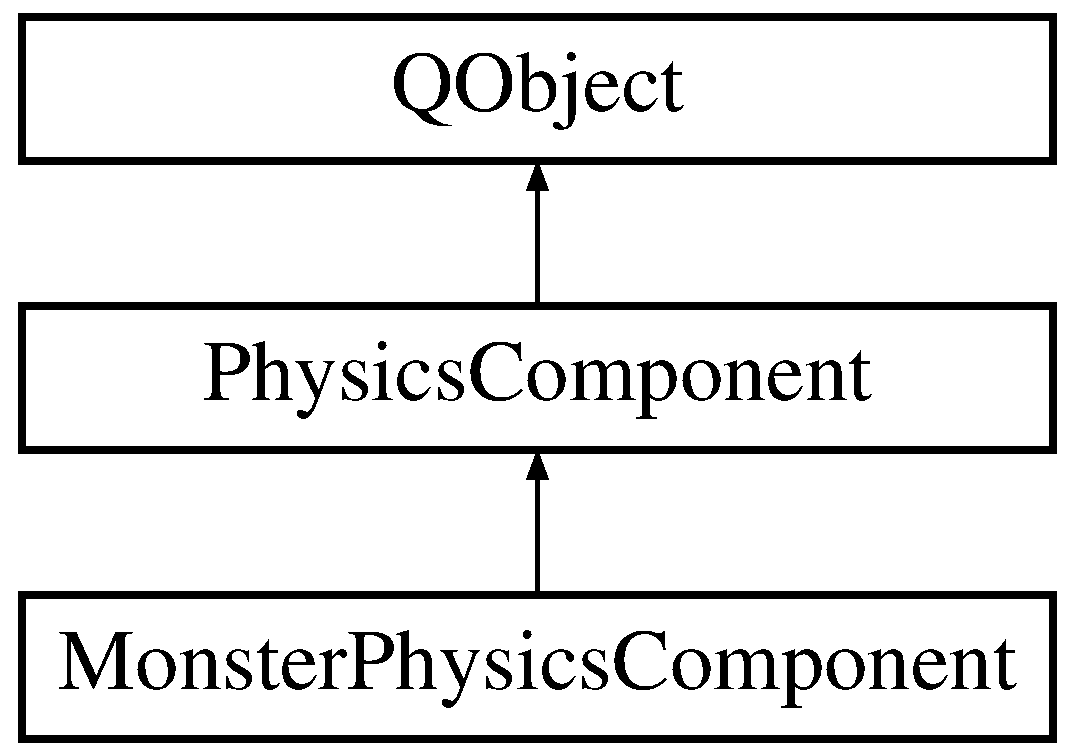
\includegraphics[height=3.000000cm]{classMonsterPhysicsComponent}
\end{center}
\end{figure}
\subsection*{Public Member Functions}
\begin{DoxyCompactItemize}
\item 
\hyperlink{classMonsterPhysicsComponent_a38c2ebc955ad3ac8fc03b0fa6452ed6e}{Monster\-Physics\-Component} (std\-::vector$<$ std\-::vector$<$ \hyperlink{classTile}{Tile} $\ast$ $>$ $>$ \&Tilesmap, qreal theight, qreal twidth, qreal sheight, qreal swidth, int fraction\-\_\-of\-\_\-speed)
\begin{DoxyCompactList}\small\item\em Constructor. \end{DoxyCompactList}\item 
\hypertarget{classMonsterPhysicsComponent_a23a31d1b31465e71f3851ad01559b0fa}{virtual \hyperlink{classMonsterPhysicsComponent_a23a31d1b31465e71f3851ad01559b0fa}{$\sim$\-Monster\-Physics\-Component} ()}\label{classMonsterPhysicsComponent_a23a31d1b31465e71f3851ad01559b0fa}

\begin{DoxyCompactList}\small\item\em Destructor. \end{DoxyCompactList}\item 
void \hyperlink{classMonsterPhysicsComponent_a590efe1034e71fa0dc039d547926e2f2}{update} (\hyperlink{classGameObject}{Game\-Object} \&game\-Object)
\begin{DoxyCompactList}\small\item\em Update the position of the monster based on \hyperlink{classState}{State} and surroundings. \end{DoxyCompactList}\end{DoxyCompactItemize}
\subsection*{Additional Inherited Members}


\subsection{Detailed Description}
Component to handle the physics for monster \hyperlink{classGameObject}{Game\-Object} objects Handles movement and position update of monsters based on \hyperlink{classState}{State}. 

\subsection{Constructor \& Destructor Documentation}
\hypertarget{classMonsterPhysicsComponent_a38c2ebc955ad3ac8fc03b0fa6452ed6e}{\index{Monster\-Physics\-Component@{Monster\-Physics\-Component}!Monster\-Physics\-Component@{Monster\-Physics\-Component}}
\index{Monster\-Physics\-Component@{Monster\-Physics\-Component}!MonsterPhysicsComponent@{Monster\-Physics\-Component}}
\subsubsection[{Monster\-Physics\-Component}]{\setlength{\rightskip}{0pt plus 5cm}Monster\-Physics\-Component\-::\-Monster\-Physics\-Component (
\begin{DoxyParamCaption}
\item[{std\-::vector$<$ std\-::vector$<$ {\bf Tile} $\ast$ $>$ $>$ \&}]{Tilesmap, }
\item[{qreal}]{theight, }
\item[{qreal}]{twidth, }
\item[{qreal}]{sheight, }
\item[{qreal}]{swidth, }
\item[{int}]{fraction\-\_\-of\-\_\-speed}
\end{DoxyParamCaption}
)}}\label{classMonsterPhysicsComponent_a38c2ebc955ad3ac8fc03b0fa6452ed6e}


Constructor. 


\begin{DoxyParams}{Parameters}
{\em Tilesmap} & the tile map of the game \\
\hline
{\em theight} & height of a tile \\
\hline
{\em twidth} & width of a tile \\
\hline
{\em sheight} & height of the screen \\
\hline
{\em swidth} & width of the screen \\
\hline
{\em fraction\-\_\-of\-\_\-speed} & fraction of total frames the monster moves \\
\hline
\end{DoxyParams}


\subsection{Member Function Documentation}
\hypertarget{classMonsterPhysicsComponent_a590efe1034e71fa0dc039d547926e2f2}{\index{Monster\-Physics\-Component@{Monster\-Physics\-Component}!update@{update}}
\index{update@{update}!MonsterPhysicsComponent@{Monster\-Physics\-Component}}
\subsubsection[{update}]{\setlength{\rightskip}{0pt plus 5cm}void Monster\-Physics\-Component\-::update (
\begin{DoxyParamCaption}
\item[{{\bf Game\-Object} \&}]{game\-Object}
\end{DoxyParamCaption}
)\hspace{0.3cm}{\ttfamily [virtual]}}}\label{classMonsterPhysicsComponent_a590efe1034e71fa0dc039d547926e2f2}


Update the position of the monster based on \hyperlink{classState}{State} and surroundings. 


\begin{DoxyParams}{Parameters}
{\em game\-Object} & the \hyperlink{classGameObject}{Game\-Object} of the monster \\
\hline
\end{DoxyParams}


Implements \hyperlink{classPhysicsComponent_a5498919fee09ce15271a5c273c2dc836}{Physics\-Component}.



The documentation for this class was generated from the following file\-:\begin{DoxyCompactItemize}
\item 
monsterphysicscomponent.\-h\end{DoxyCompactItemize}

\hypertarget{classMovingLeft}{\section{Moving\-Left Class Reference}
\label{classMovingLeft}\index{Moving\-Left@{Moving\-Left}}
}


The state in which the player is moving left This also handles the responds to key press and key release inputs so as to change the state of the \hyperlink{classGameObject}{Game\-Object}.  




{\ttfamily \#include $<$movingleft.\-h$>$}

Inheritance diagram for Moving\-Left\-:\begin{figure}[H]
\begin{center}
\leavevmode
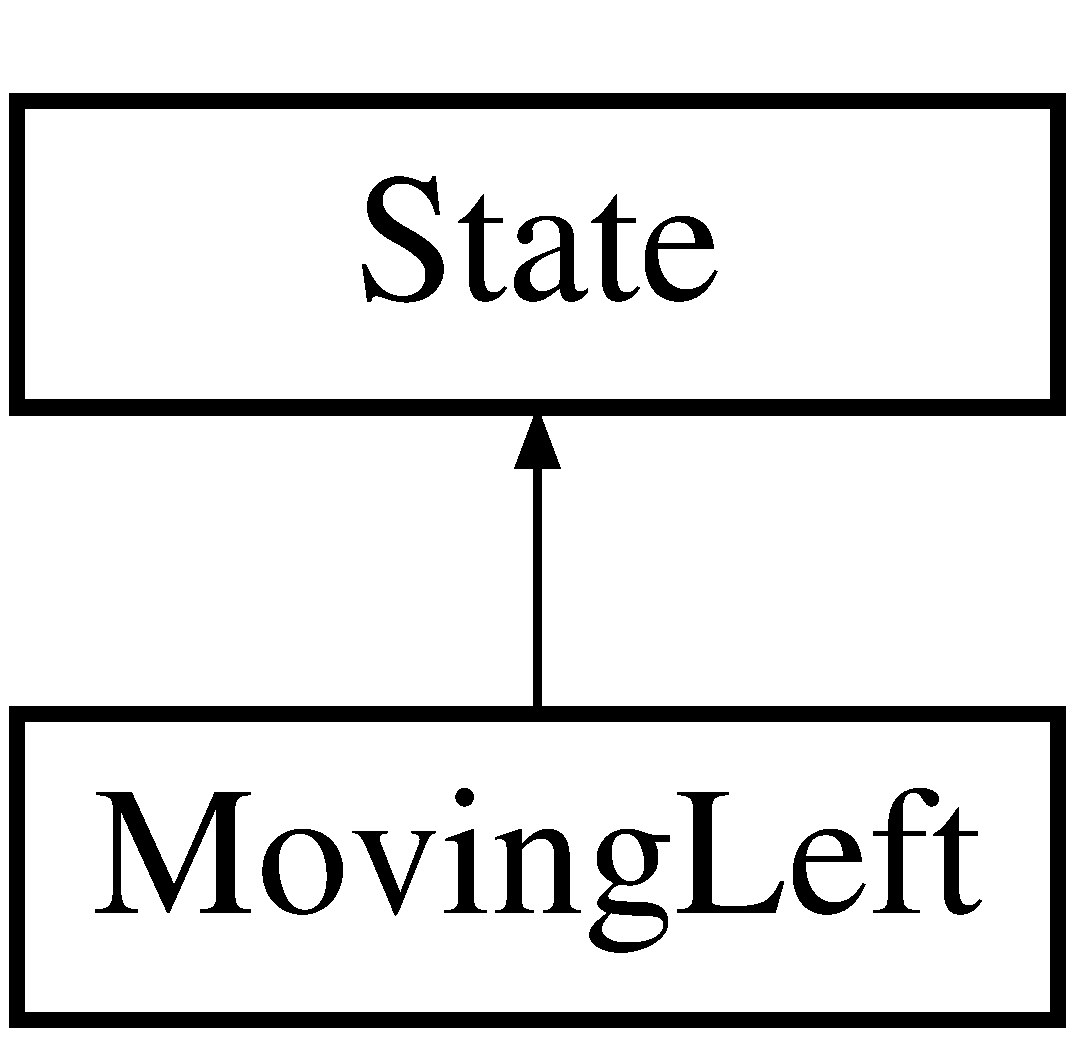
\includegraphics[height=2.000000cm]{classMovingLeft}
\end{center}
\end{figure}
\subsection*{Public Member Functions}
\begin{DoxyCompactItemize}
\item 
\hypertarget{classMovingLeft_a8a89983c75d13fa11e54299944ac79db}{\hyperlink{classMovingLeft_a8a89983c75d13fa11e54299944ac79db}{Moving\-Left} ()}\label{classMovingLeft_a8a89983c75d13fa11e54299944ac79db}

\begin{DoxyCompactList}\small\item\em Constructor. \end{DoxyCompactList}\item 
\hypertarget{classMovingLeft_a01d8becd5f957652c3a2e6e69d261bf1}{virtual \hyperlink{classMovingLeft_a01d8becd5f957652c3a2e6e69d261bf1}{$\sim$\-Moving\-Left} ()}\label{classMovingLeft_a01d8becd5f957652c3a2e6e69d261bf1}

\begin{DoxyCompactList}\small\item\em Destructor. \end{DoxyCompactList}\item 
virtual \hyperlink{classState}{State} $\ast$ \hyperlink{classMovingLeft_a0ddbc7a065b820e06caa76c650ab6765}{update} (\hyperlink{classInputComponent}{Input\-Component} $\ast$input\-Component, std\-::set$<$ Qt\-::\-Key $>$ key)
\begin{DoxyCompactList}\small\item\em Updates the state on the basis of the keys currently pressed. \end{DoxyCompactList}\item 
virtual \hyperlink{namespaceenumerator_a5fc7b342c2c633e1037b07cea237a222}{enumerator\-::\-State} \hyperlink{classMovingLeft_a2bf0f28568b5188d4b9bad622b52e47d}{type} ()
\begin{DoxyCompactList}\small\item\em Provides the type of the \hyperlink{classState}{State}, i.\-e., \hyperlink{classDeadLeft}{Dead\-Left}. \end{DoxyCompactList}\end{DoxyCompactItemize}


\subsection{Detailed Description}
The state in which the player is moving left This also handles the responds to key press and key release inputs so as to change the state of the \hyperlink{classGameObject}{Game\-Object}. 

\subsection{Member Function Documentation}
\hypertarget{classMovingLeft_a2bf0f28568b5188d4b9bad622b52e47d}{\index{Moving\-Left@{Moving\-Left}!type@{type}}
\index{type@{type}!MovingLeft@{Moving\-Left}}
\subsubsection[{type}]{\setlength{\rightskip}{0pt plus 5cm}virtual {\bf enumerator\-::\-State} Moving\-Left\-::type (
\begin{DoxyParamCaption}
{}
\end{DoxyParamCaption}
)\hspace{0.3cm}{\ttfamily [virtual]}}}\label{classMovingLeft_a2bf0f28568b5188d4b9bad622b52e47d}


Provides the type of the \hyperlink{classState}{State}, i.\-e., \hyperlink{classDeadLeft}{Dead\-Left}. 

\begin{DoxyReturn}{Returns}
enumerator\-::\-State\-::\-M\-O\-V\-I\-N\-G\-\_\-\-L\-E\-F\-T 
\end{DoxyReturn}


Implements \hyperlink{classState_a8c6cc1ff1ecdf88e586f857339b7e071}{State}.

\hypertarget{classMovingLeft_a0ddbc7a065b820e06caa76c650ab6765}{\index{Moving\-Left@{Moving\-Left}!update@{update}}
\index{update@{update}!MovingLeft@{Moving\-Left}}
\subsubsection[{update}]{\setlength{\rightskip}{0pt plus 5cm}virtual {\bf State}$\ast$ Moving\-Left\-::update (
\begin{DoxyParamCaption}
\item[{{\bf Input\-Component} $\ast$}]{input\-Component, }
\item[{std\-::set$<$ Qt\-::\-Key $>$}]{key}
\end{DoxyParamCaption}
)\hspace{0.3cm}{\ttfamily [virtual]}}}\label{classMovingLeft_a0ddbc7a065b820e06caa76c650ab6765}


Updates the state on the basis of the keys currently pressed. 


\begin{DoxyParams}{Parameters}
{\em input\-Component} & the \hyperlink{classInputComponent}{Input\-Component} of the \hyperlink{classGameObject}{Game\-Object} whose state is being updated \\
\hline
{\em key} & the set of keys currently pressed \\
\hline
\end{DoxyParams}
\begin{DoxyReturn}{Returns}
the new state 
\end{DoxyReturn}


Implements \hyperlink{classState_a5f2bc9804614c5ca9e7feb7d8c57668d}{State}.



The documentation for this class was generated from the following file\-:\begin{DoxyCompactItemize}
\item 
movingleft.\-h\end{DoxyCompactItemize}

\hypertarget{classMovingRight}{\section{Moving\-Right Class Reference}
\label{classMovingRight}\index{Moving\-Right@{Moving\-Right}}
}


The state in which the player is moving right This also handles the responds to key press and key release inputs so as to change the state of the \hyperlink{classGameObject}{Game\-Object}.  




{\ttfamily \#include $<$movingright.\-h$>$}

Inheritance diagram for Moving\-Right\-:\begin{figure}[H]
\begin{center}
\leavevmode
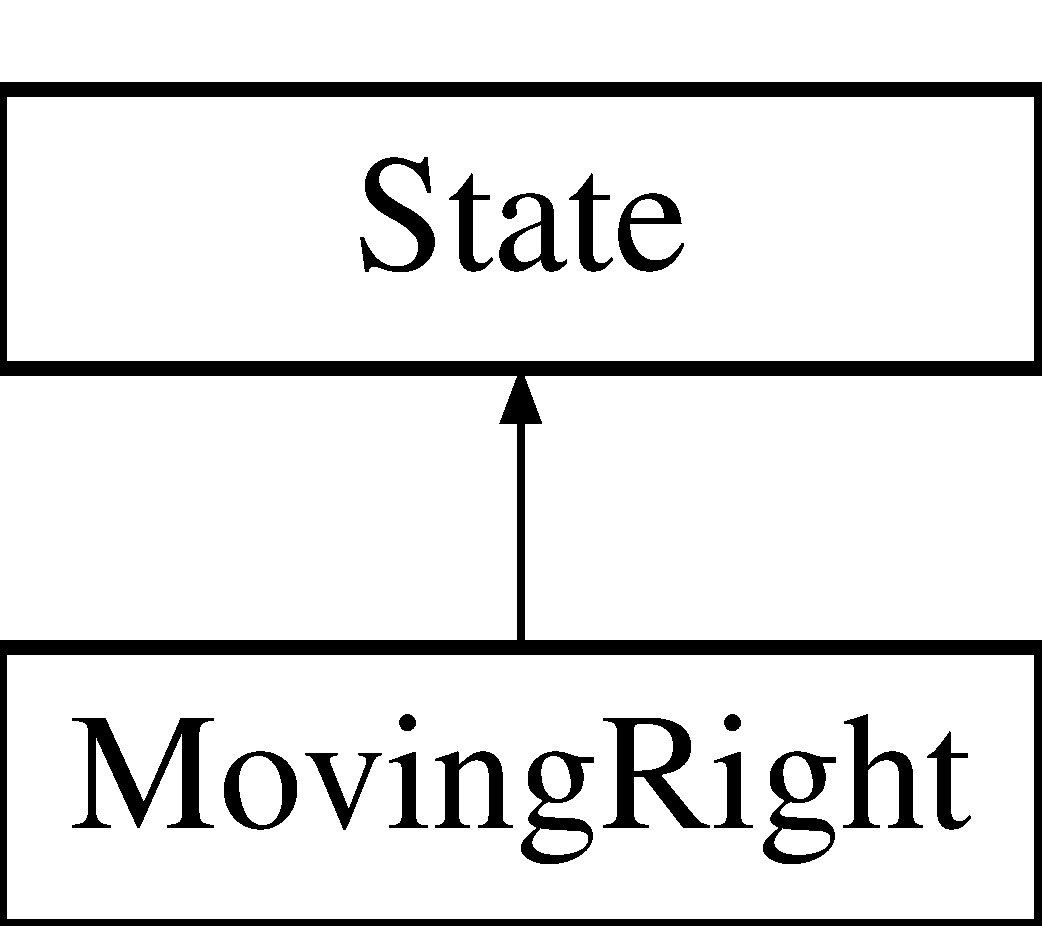
\includegraphics[height=2.000000cm]{classMovingRight}
\end{center}
\end{figure}
\subsection*{Public Member Functions}
\begin{DoxyCompactItemize}
\item 
\hypertarget{classMovingRight_a7e0aedcb305334cb740216e8ff5bf9cc}{\hyperlink{classMovingRight_a7e0aedcb305334cb740216e8ff5bf9cc}{Moving\-Right} ()}\label{classMovingRight_a7e0aedcb305334cb740216e8ff5bf9cc}

\begin{DoxyCompactList}\small\item\em Constructor. \end{DoxyCompactList}\item 
\hypertarget{classMovingRight_a9558cd656fb789be52081d7798ca3bc4}{virtual \hyperlink{classMovingRight_a9558cd656fb789be52081d7798ca3bc4}{$\sim$\-Moving\-Right} ()}\label{classMovingRight_a9558cd656fb789be52081d7798ca3bc4}

\begin{DoxyCompactList}\small\item\em Destructor. \end{DoxyCompactList}\item 
virtual \hyperlink{classState}{State} $\ast$ \hyperlink{classMovingRight_aa3ccaf974ea8137e77a26cb3738345c1}{update} (\hyperlink{classInputComponent}{Input\-Component} $\ast$input\-Component, std\-::set$<$ Qt\-::\-Key $>$ key)
\begin{DoxyCompactList}\small\item\em Updates the state on the basis of the keys currently pressed. \end{DoxyCompactList}\item 
virtual \hyperlink{namespaceenumerator_a5fc7b342c2c633e1037b07cea237a222}{enumerator\-::\-State} \hyperlink{classMovingRight_a9d8e60b64a11346a518e222ae36366ca}{type} ()
\begin{DoxyCompactList}\small\item\em Provides the type of the \hyperlink{classState}{State}, i.\-e., \hyperlink{classDeadLeft}{Dead\-Left}. \end{DoxyCompactList}\end{DoxyCompactItemize}


\subsection{Detailed Description}
The state in which the player is moving right This also handles the responds to key press and key release inputs so as to change the state of the \hyperlink{classGameObject}{Game\-Object}. 

\subsection{Member Function Documentation}
\hypertarget{classMovingRight_a9d8e60b64a11346a518e222ae36366ca}{\index{Moving\-Right@{Moving\-Right}!type@{type}}
\index{type@{type}!MovingRight@{Moving\-Right}}
\subsubsection[{type}]{\setlength{\rightskip}{0pt plus 5cm}virtual {\bf enumerator\-::\-State} Moving\-Right\-::type (
\begin{DoxyParamCaption}
{}
\end{DoxyParamCaption}
)\hspace{0.3cm}{\ttfamily [virtual]}}}\label{classMovingRight_a9d8e60b64a11346a518e222ae36366ca}


Provides the type of the \hyperlink{classState}{State}, i.\-e., \hyperlink{classDeadLeft}{Dead\-Left}. 

\begin{DoxyReturn}{Returns}
enumerator\-::\-State\-::\-M\-O\-V\-I\-N\-G\-\_\-\-R\-I\-G\-H\-T 
\end{DoxyReturn}


Implements \hyperlink{classState_a8c6cc1ff1ecdf88e586f857339b7e071}{State}.

\hypertarget{classMovingRight_aa3ccaf974ea8137e77a26cb3738345c1}{\index{Moving\-Right@{Moving\-Right}!update@{update}}
\index{update@{update}!MovingRight@{Moving\-Right}}
\subsubsection[{update}]{\setlength{\rightskip}{0pt plus 5cm}virtual {\bf State}$\ast$ Moving\-Right\-::update (
\begin{DoxyParamCaption}
\item[{{\bf Input\-Component} $\ast$}]{input\-Component, }
\item[{std\-::set$<$ Qt\-::\-Key $>$}]{key}
\end{DoxyParamCaption}
)\hspace{0.3cm}{\ttfamily [virtual]}}}\label{classMovingRight_aa3ccaf974ea8137e77a26cb3738345c1}


Updates the state on the basis of the keys currently pressed. 


\begin{DoxyParams}{Parameters}
{\em input\-Component} & the \hyperlink{classInputComponent}{Input\-Component} of the \hyperlink{classGameObject}{Game\-Object} whose state is being updated \\
\hline
{\em key} & the set of keys currently pressed \\
\hline
\end{DoxyParams}
\begin{DoxyReturn}{Returns}
the new state 
\end{DoxyReturn}


Implements \hyperlink{classState_a5f2bc9804614c5ca9e7feb7d8c57668d}{State}.



The documentation for this class was generated from the following file\-:\begin{DoxyCompactItemize}
\item 
movingright.\-h\end{DoxyCompactItemize}

\hypertarget{classPhysicsComponent}{\section{Physics\-Component Class Reference}
\label{classPhysicsComponent}\index{Physics\-Component@{Physics\-Component}}
}


Component that governs the physics handling of the \hyperlink{classGameObject}{Game\-Object} Handles the movement of the \hyperlink{classGameObject}{Game\-Object}, and sets the position on the scene based on the \hyperlink{classState}{State}.  




{\ttfamily \#include $<$physicscomponent.\-h$>$}

Inheritance diagram for Physics\-Component\-:\begin{figure}[H]
\begin{center}
\leavevmode
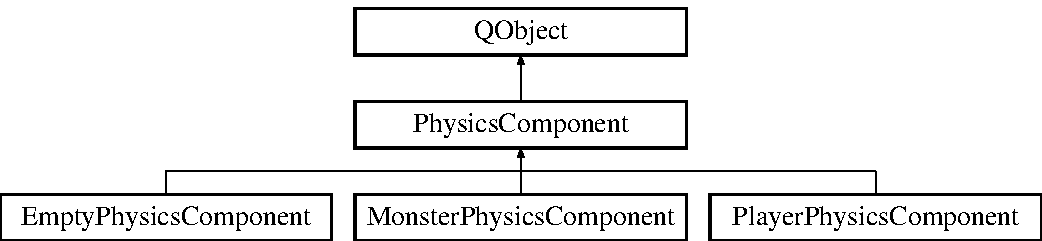
\includegraphics[height=3.000000cm]{classPhysicsComponent}
\end{center}
\end{figure}
\subsection*{Public Member Functions}
\begin{DoxyCompactItemize}
\item 
\hypertarget{classPhysicsComponent_aeb544a2a04cde8f050c6a51ec436ec4e}{\hyperlink{classPhysicsComponent_aeb544a2a04cde8f050c6a51ec436ec4e}{Physics\-Component} ()}\label{classPhysicsComponent_aeb544a2a04cde8f050c6a51ec436ec4e}

\begin{DoxyCompactList}\small\item\em Constructor. \end{DoxyCompactList}\item 
\hypertarget{classPhysicsComponent_afadf481ee69c12d205435ede58da6121}{virtual \hyperlink{classPhysicsComponent_afadf481ee69c12d205435ede58da6121}{$\sim$\-Physics\-Component} ()}\label{classPhysicsComponent_afadf481ee69c12d205435ede58da6121}

\begin{DoxyCompactList}\small\item\em Destructor. \end{DoxyCompactList}\item 
\hypertarget{classPhysicsComponent_a5498919fee09ce15271a5c273c2dc836}{virtual void \hyperlink{classPhysicsComponent_a5498919fee09ce15271a5c273c2dc836}{update} (\hyperlink{classGameObject}{Game\-Object} \&)=0}\label{classPhysicsComponent_a5498919fee09ce15271a5c273c2dc836}

\begin{DoxyCompactList}\small\item\em Updates the \hyperlink{classGameObject}{Game\-Object} object's position based on \hyperlink{classState}{State}. \end{DoxyCompactList}\item 
bool \hyperlink{classPhysicsComponent_a75cfebb94e323fd00935c369b2b8e11f}{in\-Range} (Q\-Point\-F point)
\begin{DoxyCompactList}\small\item\em Checks whether it is valid for \hyperlink{classGameObject}{Game\-Object} to be at point. \end{DoxyCompactList}\item 
bool \hyperlink{classPhysicsComponent_ab8dc7351bb7ac17177840669ef6abaaa}{test\-Point} (Q\-Point\-F point)
\begin{DoxyCompactList}\small\item\em Checks whether it is valid for \hyperlink{classGameObject}{Game\-Object} to be at point. \end{DoxyCompactList}\item 
bool \hyperlink{classPhysicsComponent_ae0c5998a85b314cb5ea324f509f919a8}{test\-Position\-For\-Player} (Q\-Point\-F input\-\_\-point, qreal player\-\_\-width, qreal player\-\_\-height)
\begin{DoxyCompactList}\small\item\em Check if a \hyperlink{classGameObject}{Game\-Object} can be placed at point such that all the points it covers are valid. \end{DoxyCompactList}\item 
bool \hyperlink{classPhysicsComponent_a2f2fab8cd26c709f50d44d404455f700}{has\-No\-Platform\-Under} (\hyperlink{classGameObject}{Game\-Object} \&game\-Object)
\begin{DoxyCompactList}\small\item\em Check whether game\-Object would start falling. \end{DoxyCompactList}\item 
bool \hyperlink{classPhysicsComponent_a552bad9336bf5cf9e9ee73c685a53edd}{has\-Obstacle\-In\-Front} (\hyperlink{classGameObject}{Game\-Object} \&game\-Object)
\begin{DoxyCompactList}\small\item\em Check whether game\-Object has an obstacle right in front of it. \end{DoxyCompactList}\end{DoxyCompactItemize}
\subsection*{Protected Attributes}
\begin{DoxyCompactItemize}
\item 
\hypertarget{classPhysicsComponent_aa1d5e5b95523225244e36df0f7490465}{std\-::vector$<$ std\-::vector$<$ \hyperlink{classTile}{Tile} $\ast$ $>$ $>$ \hyperlink{classPhysicsComponent_aa1d5e5b95523225244e36df0f7490465}{tiles\-Map}}\label{classPhysicsComponent_aa1d5e5b95523225244e36df0f7490465}

\begin{DoxyCompactList}\small\item\em Stores the tile map of the game. \end{DoxyCompactList}\item 
\hypertarget{classPhysicsComponent_a838b5b49b38cfaf7a1a4b4ab2ff6accd}{Q\-Graphics\-Scene $\ast$ \hyperlink{classPhysicsComponent_a838b5b49b38cfaf7a1a4b4ab2ff6accd}{scene}}\label{classPhysicsComponent_a838b5b49b38cfaf7a1a4b4ab2ff6accd}

\begin{DoxyCompactList}\small\item\em Stores the scene of the game. \end{DoxyCompactList}\item 
\hypertarget{classPhysicsComponent_aafd178b1852f4907462b02236675bc8e}{qreal \hyperlink{classPhysicsComponent_aafd178b1852f4907462b02236675bc8e}{width\-\_\-of\-\_\-tile}}\label{classPhysicsComponent_aafd178b1852f4907462b02236675bc8e}

\begin{DoxyCompactList}\small\item\em Width of a tile in the tile map. \end{DoxyCompactList}\item 
\hypertarget{classPhysicsComponent_af2fccaddf29b9d7beb69e90877d3f6b1}{qreal \hyperlink{classPhysicsComponent_af2fccaddf29b9d7beb69e90877d3f6b1}{height\-\_\-of\-\_\-tile}}\label{classPhysicsComponent_af2fccaddf29b9d7beb69e90877d3f6b1}

\begin{DoxyCompactList}\small\item\em Height of a tile in the tile map. \end{DoxyCompactList}\item 
\hypertarget{classPhysicsComponent_abb107c2629e5fa404b0ec29517ead1fe}{qreal \hyperlink{classPhysicsComponent_abb107c2629e5fa404b0ec29517ead1fe}{screen\-Width}}\label{classPhysicsComponent_abb107c2629e5fa404b0ec29517ead1fe}

\begin{DoxyCompactList}\small\item\em Width of the window in which the game runs. \end{DoxyCompactList}\item 
\hypertarget{classPhysicsComponent_a1541f4f1eb4a7e231683f2769ed397f3}{qreal \hyperlink{classPhysicsComponent_a1541f4f1eb4a7e231683f2769ed397f3}{screen\-Height}}\label{classPhysicsComponent_a1541f4f1eb4a7e231683f2769ed397f3}

\begin{DoxyCompactList}\small\item\em Height of the window in which the game runs. \end{DoxyCompactList}\item 
\hypertarget{classPhysicsComponent_ae88a255f60e8d4bcaab4b431d6744562}{int \hyperlink{classPhysicsComponent_ae88a255f60e8d4bcaab4b431d6744562}{cur\-Jump\-Count}}\label{classPhysicsComponent_ae88a255f60e8d4bcaab4b431d6744562}

\begin{DoxyCompactList}\small\item\em Stores the number of frames more the object will move up when jumping. \end{DoxyCompactList}\item 
\hypertarget{classPhysicsComponent_af619d6984f110bb81bdfe5889d1ef431}{int \hyperlink{classPhysicsComponent_af619d6984f110bb81bdfe5889d1ef431}{max\-Jump\-Count}}\label{classPhysicsComponent_af619d6984f110bb81bdfe5889d1ef431}

\begin{DoxyCompactList}\small\item\em Stores the total number of tiles the object moves up when jumping. \end{DoxyCompactList}\end{DoxyCompactItemize}


\subsection{Detailed Description}
Component that governs the physics handling of the \hyperlink{classGameObject}{Game\-Object} Handles the movement of the \hyperlink{classGameObject}{Game\-Object}, and sets the position on the scene based on the \hyperlink{classState}{State}. 

\subsection{Member Function Documentation}
\hypertarget{classPhysicsComponent_a2f2fab8cd26c709f50d44d404455f700}{\index{Physics\-Component@{Physics\-Component}!has\-No\-Platform\-Under@{has\-No\-Platform\-Under}}
\index{has\-No\-Platform\-Under@{has\-No\-Platform\-Under}!PhysicsComponent@{Physics\-Component}}
\subsubsection[{has\-No\-Platform\-Under}]{\setlength{\rightskip}{0pt plus 5cm}bool Physics\-Component\-::has\-No\-Platform\-Under (
\begin{DoxyParamCaption}
\item[{{\bf Game\-Object} \&}]{game\-Object}
\end{DoxyParamCaption}
)}}\label{classPhysicsComponent_a2f2fab8cd26c709f50d44d404455f700}


Check whether game\-Object would start falling. 


\begin{DoxyParams}{Parameters}
{\em game\-Object} & the \hyperlink{classGameObject}{Game\-Object} to test on \\
\hline
\end{DoxyParams}
\begin{DoxyReturn}{Returns}
true if not, false otherwise 
\end{DoxyReturn}
\hypertarget{classPhysicsComponent_a552bad9336bf5cf9e9ee73c685a53edd}{\index{Physics\-Component@{Physics\-Component}!has\-Obstacle\-In\-Front@{has\-Obstacle\-In\-Front}}
\index{has\-Obstacle\-In\-Front@{has\-Obstacle\-In\-Front}!PhysicsComponent@{Physics\-Component}}
\subsubsection[{has\-Obstacle\-In\-Front}]{\setlength{\rightskip}{0pt plus 5cm}bool Physics\-Component\-::has\-Obstacle\-In\-Front (
\begin{DoxyParamCaption}
\item[{{\bf Game\-Object} \&}]{game\-Object}
\end{DoxyParamCaption}
)}}\label{classPhysicsComponent_a552bad9336bf5cf9e9ee73c685a53edd}


Check whether game\-Object has an obstacle right in front of it. 


\begin{DoxyParams}{Parameters}
{\em game\-Object} & the \hyperlink{classGameObject}{Game\-Object} to test on \\
\hline
\end{DoxyParams}
\begin{DoxyReturn}{Returns}
true if yes, false otherwise 
\end{DoxyReturn}
\hypertarget{classPhysicsComponent_a75cfebb94e323fd00935c369b2b8e11f}{\index{Physics\-Component@{Physics\-Component}!in\-Range@{in\-Range}}
\index{in\-Range@{in\-Range}!PhysicsComponent@{Physics\-Component}}
\subsubsection[{in\-Range}]{\setlength{\rightskip}{0pt plus 5cm}bool Physics\-Component\-::in\-Range (
\begin{DoxyParamCaption}
\item[{Q\-Point\-F}]{point}
\end{DoxyParamCaption}
)}}\label{classPhysicsComponent_a75cfebb94e323fd00935c369b2b8e11f}


Checks whether it is valid for \hyperlink{classGameObject}{Game\-Object} to be at point. 


\begin{DoxyParams}{Parameters}
{\em point} & the point to be checked \\
\hline
\end{DoxyParams}
\begin{DoxyReturn}{Returns}
true, if valid position in tile map free of obstacles, false otherwise 
\end{DoxyReturn}
\hypertarget{classPhysicsComponent_ab8dc7351bb7ac17177840669ef6abaaa}{\index{Physics\-Component@{Physics\-Component}!test\-Point@{test\-Point}}
\index{test\-Point@{test\-Point}!PhysicsComponent@{Physics\-Component}}
\subsubsection[{test\-Point}]{\setlength{\rightskip}{0pt plus 5cm}bool Physics\-Component\-::test\-Point (
\begin{DoxyParamCaption}
\item[{Q\-Point\-F}]{point}
\end{DoxyParamCaption}
)}}\label{classPhysicsComponent_ab8dc7351bb7ac17177840669ef6abaaa}


Checks whether it is valid for \hyperlink{classGameObject}{Game\-Object} to be at point. 


\begin{DoxyParams}{Parameters}
{\em point} & the point to be checked \\
\hline
\end{DoxyParams}
\begin{DoxyReturn}{Returns}
true, if valid position in tile map free of obstacles, false otherwise 
\end{DoxyReturn}
\hypertarget{classPhysicsComponent_ae0c5998a85b314cb5ea324f509f919a8}{\index{Physics\-Component@{Physics\-Component}!test\-Position\-For\-Player@{test\-Position\-For\-Player}}
\index{test\-Position\-For\-Player@{test\-Position\-For\-Player}!PhysicsComponent@{Physics\-Component}}
\subsubsection[{test\-Position\-For\-Player}]{\setlength{\rightskip}{0pt plus 5cm}bool Physics\-Component\-::test\-Position\-For\-Player (
\begin{DoxyParamCaption}
\item[{Q\-Point\-F}]{input\-\_\-point, }
\item[{qreal}]{player\-\_\-width, }
\item[{qreal}]{player\-\_\-height}
\end{DoxyParamCaption}
)}}\label{classPhysicsComponent_ae0c5998a85b314cb5ea324f509f919a8}


Check if a \hyperlink{classGameObject}{Game\-Object} can be placed at point such that all the points it covers are valid. 


\begin{DoxyParams}{Parameters}
{\em input\-\_\-point} & the point to be checked \\
\hline
{\em player\-\_\-width} & the width of the \hyperlink{classGraphicsComponent}{Graphics\-Component} of the \hyperlink{classGameObject}{Game\-Object} \\
\hline
{\em player\-\_\-height} & the height of the \hyperlink{classGraphicsComponent}{Graphics\-Component} of the \hyperlink{classGameObject}{Game\-Object} \\
\hline
\end{DoxyParams}
\begin{DoxyReturn}{Returns}
true, if valid position in tile map free of obstacles, false otherwise 
\end{DoxyReturn}


The documentation for this class was generated from the following file\-:\begin{DoxyCompactItemize}
\item 
physicscomponent.\-h\end{DoxyCompactItemize}

\hypertarget{classPlayerGraphicsComponent}{\section{Player\-Graphics\-Component Class Reference}
\label{classPlayerGraphicsComponent}\index{Player\-Graphics\-Component@{Player\-Graphics\-Component}}
}


Component to handle graphics of a \hyperlink{classGameObject}{Game\-Object} Handles how the \hyperlink{classGameObject}{Game\-Object} looks, and updates based on the \hyperlink{classState}{State}.  




{\ttfamily \#include $<$playergraphicscomponent.\-h$>$}

Inheritance diagram for Player\-Graphics\-Component\-:\begin{figure}[H]
\begin{center}
\leavevmode
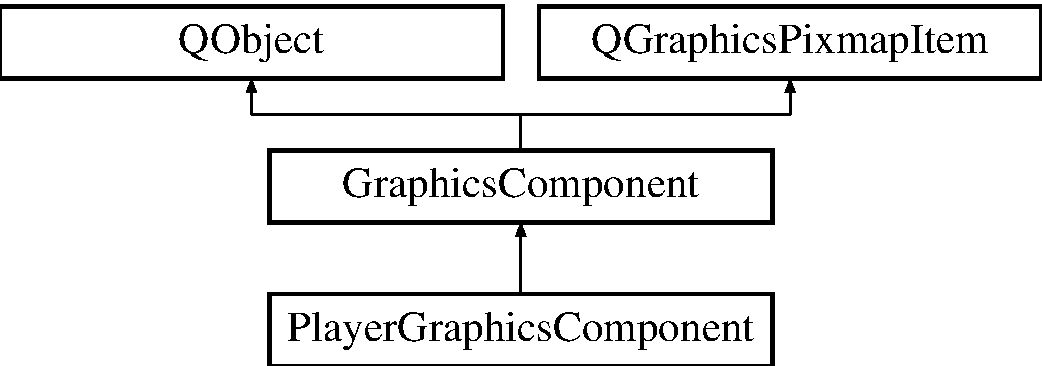
\includegraphics[height=3.000000cm]{classPlayerGraphicsComponent}
\end{center}
\end{figure}
\subsection*{Public Member Functions}
\begin{DoxyCompactItemize}
\item 
std\-::vector$<$ qreal $>$ \hyperlink{classPlayerGraphicsComponent_a9e4f6d92f14886b23791ac2eb8846349}{get\-Size\-Position\-Of\-Object} ()
\begin{DoxyCompactList}\small\item\em get left top coordinate and width and height of rectangle \end{DoxyCompactList}\item 
\hyperlink{classPlayerGraphicsComponent_a398184a4c0bc09ff5011d57359bc102b}{Player\-Graphics\-Component} (Q\-Graphics\-Scene $\ast$scene, std\-::string images\-\_\-location, std\-::vector$<$ int $>$ \&images\-\_\-total\-\_\-count, int image\-\_\-width, int image\-\_\-height, qreal x\-\_\-coordinate, qreal y\-\_\-coordinate, bool is\-\_\-dangerous, Q\-Application $\ast$a)
\begin{DoxyCompactList}\small\item\em constructor for all the images of player and monster \end{DoxyCompactList}\item 
\hypertarget{classPlayerGraphicsComponent_a9bec033acf2dc9abab5e7240e47cc98f}{\hyperlink{classPlayerGraphicsComponent_a9bec033acf2dc9abab5e7240e47cc98f}{$\sim$\-Player\-Graphics\-Component} ()}\label{classPlayerGraphicsComponent_a9bec033acf2dc9abab5e7240e47cc98f}

\begin{DoxyCompactList}\small\item\em destructor \end{DoxyCompactList}\item 
void \hyperlink{classPlayerGraphicsComponent_ace3901cc8345392c22315f24d617e98b}{update} (\hyperlink{classGameObject}{Game\-Object} \&obj)
\begin{DoxyCompactList}\small\item\em in each game loop this function is called which changes the image based on graphics\-Counter\mbox{[}\mbox{]} \end{DoxyCompactList}\item 
void \hyperlink{classPlayerGraphicsComponent_a9f5a0e1621cb9809a7aebe2927a5fad3}{set\-App} (Q\-Application $\ast$a)
\begin{DoxyCompactList}\small\item\em set\-App set the Qapplication \end{DoxyCompactList}\end{DoxyCompactItemize}
\subsection*{Additional Inherited Members}


\subsection{Detailed Description}
Component to handle graphics of a \hyperlink{classGameObject}{Game\-Object} Handles how the \hyperlink{classGameObject}{Game\-Object} looks, and updates based on the \hyperlink{classState}{State}. 

\subsection{Constructor \& Destructor Documentation}
\hypertarget{classPlayerGraphicsComponent_a398184a4c0bc09ff5011d57359bc102b}{\index{Player\-Graphics\-Component@{Player\-Graphics\-Component}!Player\-Graphics\-Component@{Player\-Graphics\-Component}}
\index{Player\-Graphics\-Component@{Player\-Graphics\-Component}!PlayerGraphicsComponent@{Player\-Graphics\-Component}}
\subsubsection[{Player\-Graphics\-Component}]{\setlength{\rightskip}{0pt plus 5cm}Player\-Graphics\-Component\-::\-Player\-Graphics\-Component (
\begin{DoxyParamCaption}
\item[{Q\-Graphics\-Scene $\ast$}]{scene, }
\item[{std\-::string}]{images\-\_\-location, }
\item[{std\-::vector$<$ int $>$ \&}]{images\-\_\-total\-\_\-count, }
\item[{int}]{image\-\_\-width, }
\item[{int}]{image\-\_\-height, }
\item[{qreal}]{x\-\_\-coordinate, }
\item[{qreal}]{y\-\_\-coordinate, }
\item[{bool}]{is\-\_\-dangerous, }
\item[{Q\-Application $\ast$}]{a}
\end{DoxyParamCaption}
)}}\label{classPlayerGraphicsComponent_a398184a4c0bc09ff5011d57359bc102b}


constructor for all the images of player and monster 


\begin{DoxyParams}{Parameters}
{\em scene} & add items to screen \\
\hline
{\em images\-\_\-location} & substring of the images location path \\
\hline
{\em images\-\_\-total\-\_\-count} & vector of total images for the different states \\
\hline
{\em image\-\_\-width} & width of all images \\
\hline
{\em image\-\_\-height} & height of all images \\
\hline
{\em x\-\_\-coordinate} & x position of image \\
\hline
{\em y\-\_\-coordinate} & y position of image \\
\hline
{\em is\-\_\-dangerous} & differentiate player and monster \\
\hline
{\em a} & Qapplication for process\-Events \\
\hline
\end{DoxyParams}


\subsection{Member Function Documentation}
\hypertarget{classPlayerGraphicsComponent_a9e4f6d92f14886b23791ac2eb8846349}{\index{Player\-Graphics\-Component@{Player\-Graphics\-Component}!get\-Size\-Position\-Of\-Object@{get\-Size\-Position\-Of\-Object}}
\index{get\-Size\-Position\-Of\-Object@{get\-Size\-Position\-Of\-Object}!PlayerGraphicsComponent@{Player\-Graphics\-Component}}
\subsubsection[{get\-Size\-Position\-Of\-Object}]{\setlength{\rightskip}{0pt plus 5cm}std\-::vector$<$qreal$>$ Player\-Graphics\-Component\-::get\-Size\-Position\-Of\-Object (
\begin{DoxyParamCaption}
{}
\end{DoxyParamCaption}
)\hspace{0.3cm}{\ttfamily [virtual]}}}\label{classPlayerGraphicsComponent_a9e4f6d92f14886b23791ac2eb8846349}


get left top coordinate and width and height of rectangle 

\begin{DoxyReturn}{Returns}
vector of image characteristics 
\end{DoxyReturn}


Implements \hyperlink{classGraphicsComponent_a653e0474dd66fc1876f405831e121631}{Graphics\-Component}.

\hypertarget{classPlayerGraphicsComponent_a9f5a0e1621cb9809a7aebe2927a5fad3}{\index{Player\-Graphics\-Component@{Player\-Graphics\-Component}!set\-App@{set\-App}}
\index{set\-App@{set\-App}!PlayerGraphicsComponent@{Player\-Graphics\-Component}}
\subsubsection[{set\-App}]{\setlength{\rightskip}{0pt plus 5cm}void Player\-Graphics\-Component\-::set\-App (
\begin{DoxyParamCaption}
\item[{Q\-Application $\ast$}]{a}
\end{DoxyParamCaption}
)}}\label{classPlayerGraphicsComponent_a9f5a0e1621cb9809a7aebe2927a5fad3}


set\-App set the Qapplication 


\begin{DoxyParams}{Parameters}
{\em a} & Qapplication \\
\hline
\end{DoxyParams}
\hypertarget{classPlayerGraphicsComponent_ace3901cc8345392c22315f24d617e98b}{\index{Player\-Graphics\-Component@{Player\-Graphics\-Component}!update@{update}}
\index{update@{update}!PlayerGraphicsComponent@{Player\-Graphics\-Component}}
\subsubsection[{update}]{\setlength{\rightskip}{0pt plus 5cm}void Player\-Graphics\-Component\-::update (
\begin{DoxyParamCaption}
\item[{{\bf Game\-Object} \&}]{obj}
\end{DoxyParamCaption}
)\hspace{0.3cm}{\ttfamily [virtual]}}}\label{classPlayerGraphicsComponent_ace3901cc8345392c22315f24d617e98b}


in each game loop this function is called which changes the image based on graphics\-Counter\mbox{[}\mbox{]} 


\begin{DoxyParams}{Parameters}
{\em obj} & player or zombie game\-Object \\
\hline
\end{DoxyParams}


Reimplemented from \hyperlink{classGraphicsComponent_a744134b79cf11b2ff29fb7802923fda9}{Graphics\-Component}.



The documentation for this class was generated from the following file\-:\begin{DoxyCompactItemize}
\item 
playergraphicscomponent.\-h\end{DoxyCompactItemize}

\hypertarget{classPlayerPhysicsComponent}{\section{Player\-Physics\-Component Class Reference}
\label{classPlayerPhysicsComponent}\index{Player\-Physics\-Component@{Player\-Physics\-Component}}
}


Component to handle the physics of a \hyperlink{classGameObject}{Game\-Object} that is a player Handles movement and sets position of the \hyperlink{classGameObject}{Game\-Object} based on its \hyperlink{classState}{State}.  




{\ttfamily \#include $<$playerphysicscomponent.\-h$>$}

Inheritance diagram for Player\-Physics\-Component\-:\begin{figure}[H]
\begin{center}
\leavevmode
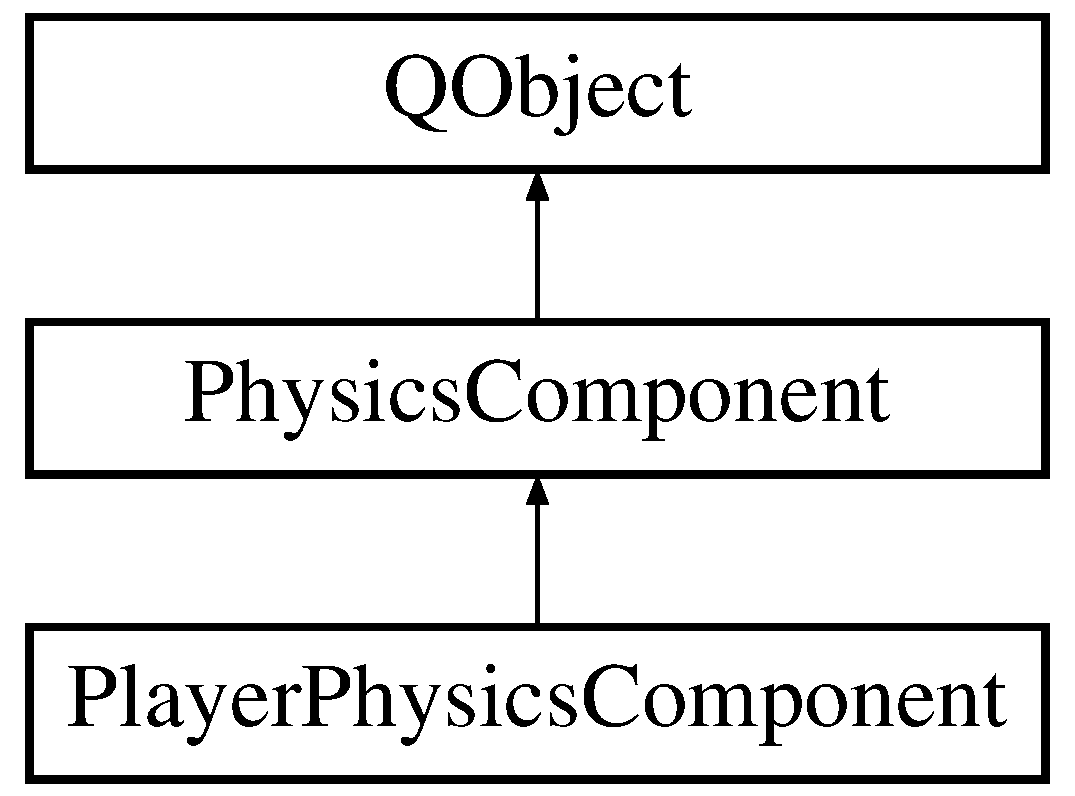
\includegraphics[height=3.000000cm]{classPlayerPhysicsComponent}
\end{center}
\end{figure}
\subsection*{Public Member Functions}
\begin{DoxyCompactItemize}
\item 
\hyperlink{classPlayerPhysicsComponent_aa369c3e7e53e11bea700b75832bab9e5}{Player\-Physics\-Component} (std\-::vector$<$ std\-::vector$<$ \hyperlink{classTile}{Tile} $\ast$ $>$ $>$ \&Tilesmap, qreal theight, qreal twidth, qreal sheight, qreal swidth, Q\-Graphics\-Scene $\ast$\hyperlink{classPhysicsComponent_a838b5b49b38cfaf7a1a4b4ab2ff6accd}{scene})
\begin{DoxyCompactList}\small\item\em Constructor. \end{DoxyCompactList}\item 
void \hyperlink{classPlayerPhysicsComponent_a637c081a84bb314c6e69a50ccdcc83f4}{update} (\hyperlink{classGameObject}{Game\-Object} \&game\-Object)
\begin{DoxyCompactList}\small\item\em Updates the positions of the \hyperlink{classGameObject}{Game\-Object} based on the \hyperlink{classState}{State}. \end{DoxyCompactList}\end{DoxyCompactItemize}
\subsection*{Additional Inherited Members}


\subsection{Detailed Description}
Component to handle the physics of a \hyperlink{classGameObject}{Game\-Object} that is a player Handles movement and sets position of the \hyperlink{classGameObject}{Game\-Object} based on its \hyperlink{classState}{State}. 

\subsection{Constructor \& Destructor Documentation}
\hypertarget{classPlayerPhysicsComponent_aa369c3e7e53e11bea700b75832bab9e5}{\index{Player\-Physics\-Component@{Player\-Physics\-Component}!Player\-Physics\-Component@{Player\-Physics\-Component}}
\index{Player\-Physics\-Component@{Player\-Physics\-Component}!PlayerPhysicsComponent@{Player\-Physics\-Component}}
\subsubsection[{Player\-Physics\-Component}]{\setlength{\rightskip}{0pt plus 5cm}Player\-Physics\-Component\-::\-Player\-Physics\-Component (
\begin{DoxyParamCaption}
\item[{std\-::vector$<$ std\-::vector$<$ {\bf Tile} $\ast$ $>$ $>$ \&}]{Tilesmap, }
\item[{qreal}]{theight, }
\item[{qreal}]{twidth, }
\item[{qreal}]{sheight, }
\item[{qreal}]{swidth, }
\item[{Q\-Graphics\-Scene $\ast$}]{scene}
\end{DoxyParamCaption}
)}}\label{classPlayerPhysicsComponent_aa369c3e7e53e11bea700b75832bab9e5}


Constructor. 


\begin{DoxyParams}{Parameters}
{\em Tilesmap} & the tile map of the game \\
\hline
{\em theight} & height of a tile \\
\hline
{\em twidth} & width of a tile \\
\hline
{\em sheight} & height of the window in which the game is played \\
\hline
{\em swidth} & width of the window in which the game is played \\
\hline
{\em scene} & scene of the game \\
\hline
\end{DoxyParams}


\subsection{Member Function Documentation}
\hypertarget{classPlayerPhysicsComponent_a637c081a84bb314c6e69a50ccdcc83f4}{\index{Player\-Physics\-Component@{Player\-Physics\-Component}!update@{update}}
\index{update@{update}!PlayerPhysicsComponent@{Player\-Physics\-Component}}
\subsubsection[{update}]{\setlength{\rightskip}{0pt plus 5cm}void Player\-Physics\-Component\-::update (
\begin{DoxyParamCaption}
\item[{{\bf Game\-Object} \&}]{game\-Object}
\end{DoxyParamCaption}
)\hspace{0.3cm}{\ttfamily [virtual]}}}\label{classPlayerPhysicsComponent_a637c081a84bb314c6e69a50ccdcc83f4}


Updates the positions of the \hyperlink{classGameObject}{Game\-Object} based on the \hyperlink{classState}{State}. 


\begin{DoxyParams}{Parameters}
{\em game\-Object} & the \hyperlink{classGameObject}{Game\-Object} to be updated \\
\hline
\end{DoxyParams}


Implements \hyperlink{classPhysicsComponent_a5498919fee09ce15271a5c273c2dc836}{Physics\-Component}.



The documentation for this class was generated from the following file\-:\begin{DoxyCompactItemize}
\item 
playerphysicscomponent.\-h\end{DoxyCompactItemize}

\hypertarget{classReadInput}{\section{Read\-Input Class Reference}
\label{classReadInput}\index{Read\-Input@{Read\-Input}}
}


Function to read input from the game files.  




{\ttfamily \#include $<$readinput.\-h$>$}

\subsection*{Public Member Functions}
\begin{DoxyCompactItemize}
\item 
\hyperlink{classReadInput_a25c8fa92ada2fb103817fb1eb1c67020}{Read\-Input} (Q\-Graphics\-Scene $\ast$\hyperlink{classReadInput_a6ef3ea2e71749ad16f4bcd0bdae740c4}{scene}, int screen\-\_\-width, int screen\-\_\-height)
\begin{DoxyCompactList}\small\item\em Constructor. \end{DoxyCompactList}\item 
\hypertarget{classReadInput_aec19e94e448ed46207c55412a61728fa}{\hyperlink{classReadInput_aec19e94e448ed46207c55412a61728fa}{$\sim$\-Read\-Input} ()}\label{classReadInput_aec19e94e448ed46207c55412a61728fa}

\begin{DoxyCompactList}\small\item\em Destructor. \end{DoxyCompactList}\item 
void \hyperlink{classReadInput_a3bf04a443a4ef1df2c1a380c81ba0f0b}{function\-To\-Create\-Tile\-Map} (std\-::string file\-\_\-path)
\begin{DoxyCompactList}\small\item\em Function to Create the \hyperlink{classTile}{Tile} Map. \end{DoxyCompactList}\item 
void \hyperlink{classReadInput_a8784d64abe0ee437915679d7d602ab10}{function\-To\-Create\-Gem} (std\-::string file\-\_\-path)
\begin{DoxyCompactList}\small\item\em Function to Create Gems. \end{DoxyCompactList}\item 
void \hyperlink{classReadInput_a1ed7e1e601b0fe876b289884c289bda5}{function\-To\-Create\-Player\-Game\-Object} (std\-::string file\-\_\-path)
\begin{DoxyCompactList}\small\item\em Function to Create The Players. \end{DoxyCompactList}\item 
void \hyperlink{classReadInput_a627c05559722971112fdc9b076234907}{function\-To\-Create\-Monster\-Game\-Object} (std\-::string file\-\_\-path)
\begin{DoxyCompactList}\small\item\em Function to Create the Monsters. \end{DoxyCompactList}\item 
void \hyperlink{classReadInput_acf8a8a99a12546eb1fd2871626411ec6}{function\-To\-Create\-Fire\-Object} (std\-::string fire\-\_\-file\-\_\-path)
\begin{DoxyCompactList}\small\item\em Function to Create Fire. \end{DoxyCompactList}\item 
void \hyperlink{classReadInput_a51ac6aba5ed863639d7cbbbd962a9996}{function\-To\-Create\-Door} (std\-::string door\-\_\-file\-\_\-path)
\begin{DoxyCompactList}\small\item\em function\-To\-Create\-Door \end{DoxyCompactList}\item 
void \hyperlink{classReadInput_a2aac5874b99ac1dc471ad8ea8ddbba8b}{set\-App} (Q\-Application $\ast$a)
\begin{DoxyCompactList}\small\item\em To set the Current Q\-Application. \end{DoxyCompactList}\end{DoxyCompactItemize}
\subsection*{Public Attributes}
\begin{DoxyCompactItemize}
\item 
\hypertarget{classReadInput_adc606d86ae9c132ab1621cee0ea75bf7}{\hyperlink{namespaceenumerator_aa4c03441b2e09279e43235eb80525c6d}{enumerator\-::\-Identity} \hyperlink{classReadInput_adc606d86ae9c132ab1621cee0ea75bf7}{remote\-Identity}}\label{classReadInput_adc606d86ae9c132ab1621cee0ea75bf7}

\begin{DoxyCompactList}\small\item\em Stores whether it is \hyperlink{classServer}{Server} or \hyperlink{classClient}{Client}. \end{DoxyCompactList}\item 
\hypertarget{classReadInput_a21ac8a09fc880cd70eb4bdfc61d05007}{std\-::vector$<$ \hyperlink{classGameObject}{Game\-Object} $\ast$ $>$ \hyperlink{classReadInput_a21ac8a09fc880cd70eb4bdfc61d05007}{game\-Object}}\label{classReadInput_a21ac8a09fc880cd70eb4bdfc61d05007}

\begin{DoxyCompactList}\small\item\em Vector Containing all the Game Objects. \end{DoxyCompactList}\item 
\hypertarget{classReadInput_a074e31396ae2e02327562d9233b6c22e}{std\-::vector$<$ std\-::vector$<$ \hyperlink{classTile}{Tile} $\ast$ $>$ $>$ \hyperlink{classReadInput_a074e31396ae2e02327562d9233b6c22e}{tile\-Map}}\label{classReadInput_a074e31396ae2e02327562d9233b6c22e}

\begin{DoxyCompactList}\small\item\em The \hyperlink{classTile}{Tile} Map Vector. \end{DoxyCompactList}\item 
\hypertarget{classReadInput_ac69175ef5ebd6c14ac491ade5a2409a8}{std\-::vector$<$ \hyperlink{classGem}{Gem} $\ast$ $>$ \hyperlink{classReadInput_ac69175ef5ebd6c14ac491ade5a2409a8}{gems}}\label{classReadInput_ac69175ef5ebd6c14ac491ade5a2409a8}

\begin{DoxyCompactList}\small\item\em vector to store all the gems \end{DoxyCompactList}\item 
\hypertarget{classReadInput_a6ef3ea2e71749ad16f4bcd0bdae740c4}{Q\-Graphics\-Scene $\ast$ \hyperlink{classReadInput_a6ef3ea2e71749ad16f4bcd0bdae740c4}{scene}}\label{classReadInput_a6ef3ea2e71749ad16f4bcd0bdae740c4}

\begin{DoxyCompactList}\small\item\em The Scene where to add all the game objects. \end{DoxyCompactList}\item 
\hypertarget{classReadInput_ac37f50f8dccc35548092fc547a696e8b}{qreal \hyperlink{classReadInput_ac37f50f8dccc35548092fc547a696e8b}{width\-\_\-of\-\_\-tile}}\label{classReadInput_ac37f50f8dccc35548092fc547a696e8b}

\begin{DoxyCompactList}\small\item\em Width of the \hyperlink{classTile}{Tile} relative to Screen Width. \end{DoxyCompactList}\item 
\hypertarget{classReadInput_a5f2147dd5ccbcfcd0bda7ad4a4223806}{qreal \hyperlink{classReadInput_a5f2147dd5ccbcfcd0bda7ad4a4223806}{height\-\_\-of\-\_\-tile}}\label{classReadInput_a5f2147dd5ccbcfcd0bda7ad4a4223806}

\begin{DoxyCompactList}\small\item\em Height of the \hyperlink{classTile}{Tile} relative to Screen Height. \end{DoxyCompactList}\item 
\hypertarget{classReadInput_a110330967ab2d06e89240eff7b933f9d}{Q\-Application $\ast$ \hyperlink{classReadInput_a110330967ab2d06e89240eff7b933f9d}{app}}\label{classReadInput_a110330967ab2d06e89240eff7b933f9d}

\begin{DoxyCompactList}\small\item\em Q\-Application. \end{DoxyCompactList}\item 
\hypertarget{classReadInput_abdeefb04b7789d19ef130522fa8eacf8}{int \hyperlink{classReadInput_abdeefb04b7789d19ef130522fa8eacf8}{screen\-Width}}\label{classReadInput_abdeefb04b7789d19ef130522fa8eacf8}

\begin{DoxyCompactList}\small\item\em Width of the Screen. \end{DoxyCompactList}\item 
\hypertarget{classReadInput_a0d6a1690d18753353603622b8ab0e99c}{int \hyperlink{classReadInput_a0d6a1690d18753353603622b8ab0e99c}{screen\-Height}}\label{classReadInput_a0d6a1690d18753353603622b8ab0e99c}

\begin{DoxyCompactList}\small\item\em Height of the Screen. \end{DoxyCompactList}\item 
\hypertarget{classReadInput_a4b07fa90c576175ceb01f7e87e7ffd96}{int \hyperlink{classReadInput_a4b07fa90c576175ceb01f7e87e7ffd96}{total\-Time}}\label{classReadInput_a4b07fa90c576175ceb01f7e87e7ffd96}

\begin{DoxyCompactList}\small\item\em Total Time before Game Ends. \end{DoxyCompactList}\end{DoxyCompactItemize}


\subsection{Detailed Description}
Function to read input from the game files. 

\subsection{Constructor \& Destructor Documentation}
\hypertarget{classReadInput_a25c8fa92ada2fb103817fb1eb1c67020}{\index{Read\-Input@{Read\-Input}!Read\-Input@{Read\-Input}}
\index{Read\-Input@{Read\-Input}!ReadInput@{Read\-Input}}
\subsubsection[{Read\-Input}]{\setlength{\rightskip}{0pt plus 5cm}Read\-Input\-::\-Read\-Input (
\begin{DoxyParamCaption}
\item[{Q\-Graphics\-Scene $\ast$}]{scene, }
\item[{int}]{screen\-\_\-width, }
\item[{int}]{screen\-\_\-height}
\end{DoxyParamCaption}
)}}\label{classReadInput_a25c8fa92ada2fb103817fb1eb1c67020}


Constructor. 


\begin{DoxyParams}{Parameters}
{\em scene} & The Scene pointer \\
\hline
{\em screen\-\_\-width} & Value of Width of Screen \\
\hline
{\em screen\-\_\-height} & Value of Height of Screen \\
\hline
\end{DoxyParams}


\subsection{Member Function Documentation}
\hypertarget{classReadInput_a51ac6aba5ed863639d7cbbbd962a9996}{\index{Read\-Input@{Read\-Input}!function\-To\-Create\-Door@{function\-To\-Create\-Door}}
\index{function\-To\-Create\-Door@{function\-To\-Create\-Door}!ReadInput@{Read\-Input}}
\subsubsection[{function\-To\-Create\-Door}]{\setlength{\rightskip}{0pt plus 5cm}void Read\-Input\-::function\-To\-Create\-Door (
\begin{DoxyParamCaption}
\item[{std\-::string}]{door\-\_\-file\-\_\-path}
\end{DoxyParamCaption}
)}}\label{classReadInput_a51ac6aba5ed863639d7cbbbd962a9996}


function\-To\-Create\-Door 


\begin{DoxyParams}{Parameters}
{\em door\-\_\-file\-\_\-path} & Path of the File containing \hyperlink{classDoor}{Door} information \\
\hline
\end{DoxyParams}
\hypertarget{classReadInput_acf8a8a99a12546eb1fd2871626411ec6}{\index{Read\-Input@{Read\-Input}!function\-To\-Create\-Fire\-Object@{function\-To\-Create\-Fire\-Object}}
\index{function\-To\-Create\-Fire\-Object@{function\-To\-Create\-Fire\-Object}!ReadInput@{Read\-Input}}
\subsubsection[{function\-To\-Create\-Fire\-Object}]{\setlength{\rightskip}{0pt plus 5cm}void Read\-Input\-::function\-To\-Create\-Fire\-Object (
\begin{DoxyParamCaption}
\item[{std\-::string}]{fire\-\_\-file\-\_\-path}
\end{DoxyParamCaption}
)}}\label{classReadInput_acf8a8a99a12546eb1fd2871626411ec6}


Function to Create Fire. 


\begin{DoxyParams}{Parameters}
{\em fire\-\_\-file\-\_\-path} & Path of the File containing Fire \\
\hline
\end{DoxyParams}
\hypertarget{classReadInput_a8784d64abe0ee437915679d7d602ab10}{\index{Read\-Input@{Read\-Input}!function\-To\-Create\-Gem@{function\-To\-Create\-Gem}}
\index{function\-To\-Create\-Gem@{function\-To\-Create\-Gem}!ReadInput@{Read\-Input}}
\subsubsection[{function\-To\-Create\-Gem}]{\setlength{\rightskip}{0pt plus 5cm}void Read\-Input\-::function\-To\-Create\-Gem (
\begin{DoxyParamCaption}
\item[{std\-::string}]{file\-\_\-path}
\end{DoxyParamCaption}
)}}\label{classReadInput_a8784d64abe0ee437915679d7d602ab10}


Function to Create Gems. 


\begin{DoxyParams}{Parameters}
{\em file\-\_\-path} & Path of the File containing information about Gems \\
\hline
\end{DoxyParams}
\hypertarget{classReadInput_a627c05559722971112fdc9b076234907}{\index{Read\-Input@{Read\-Input}!function\-To\-Create\-Monster\-Game\-Object@{function\-To\-Create\-Monster\-Game\-Object}}
\index{function\-To\-Create\-Monster\-Game\-Object@{function\-To\-Create\-Monster\-Game\-Object}!ReadInput@{Read\-Input}}
\subsubsection[{function\-To\-Create\-Monster\-Game\-Object}]{\setlength{\rightskip}{0pt plus 5cm}void Read\-Input\-::function\-To\-Create\-Monster\-Game\-Object (
\begin{DoxyParamCaption}
\item[{std\-::string}]{file\-\_\-path}
\end{DoxyParamCaption}
)}}\label{classReadInput_a627c05559722971112fdc9b076234907}


Function to Create the Monsters. 


\begin{DoxyParams}{Parameters}
{\em file\-\_\-path} & Path of the File Containing monsters \\
\hline
\end{DoxyParams}
\hypertarget{classReadInput_a1ed7e1e601b0fe876b289884c289bda5}{\index{Read\-Input@{Read\-Input}!function\-To\-Create\-Player\-Game\-Object@{function\-To\-Create\-Player\-Game\-Object}}
\index{function\-To\-Create\-Player\-Game\-Object@{function\-To\-Create\-Player\-Game\-Object}!ReadInput@{Read\-Input}}
\subsubsection[{function\-To\-Create\-Player\-Game\-Object}]{\setlength{\rightskip}{0pt plus 5cm}void Read\-Input\-::function\-To\-Create\-Player\-Game\-Object (
\begin{DoxyParamCaption}
\item[{std\-::string}]{file\-\_\-path}
\end{DoxyParamCaption}
)}}\label{classReadInput_a1ed7e1e601b0fe876b289884c289bda5}


Function to Create The Players. 


\begin{DoxyParams}{Parameters}
{\em file\-\_\-path} & Path of the File containing all the information about players \\
\hline
\end{DoxyParams}
\hypertarget{classReadInput_a3bf04a443a4ef1df2c1a380c81ba0f0b}{\index{Read\-Input@{Read\-Input}!function\-To\-Create\-Tile\-Map@{function\-To\-Create\-Tile\-Map}}
\index{function\-To\-Create\-Tile\-Map@{function\-To\-Create\-Tile\-Map}!ReadInput@{Read\-Input}}
\subsubsection[{function\-To\-Create\-Tile\-Map}]{\setlength{\rightskip}{0pt plus 5cm}void Read\-Input\-::function\-To\-Create\-Tile\-Map (
\begin{DoxyParamCaption}
\item[{std\-::string}]{file\-\_\-path}
\end{DoxyParamCaption}
)}}\label{classReadInput_a3bf04a443a4ef1df2c1a380c81ba0f0b}


Function to Create the \hyperlink{classTile}{Tile} Map. 


\begin{DoxyParams}{Parameters}
{\em file\-\_\-path} & Path of File containing information of \hyperlink{classTile}{Tile} Map \\
\hline
\end{DoxyParams}
\hypertarget{classReadInput_a2aac5874b99ac1dc471ad8ea8ddbba8b}{\index{Read\-Input@{Read\-Input}!set\-App@{set\-App}}
\index{set\-App@{set\-App}!ReadInput@{Read\-Input}}
\subsubsection[{set\-App}]{\setlength{\rightskip}{0pt plus 5cm}void Read\-Input\-::set\-App (
\begin{DoxyParamCaption}
\item[{Q\-Application $\ast$}]{a}
\end{DoxyParamCaption}
)}}\label{classReadInput_a2aac5874b99ac1dc471ad8ea8ddbba8b}


To set the Current Q\-Application. 


\begin{DoxyParams}{Parameters}
{\em Q\-Application} & Pointer \\
\hline
\end{DoxyParams}


The documentation for this class was generated from the following file\-:\begin{DoxyCompactItemize}
\item 
readinput.\-h\end{DoxyCompactItemize}

\hypertarget{classScoreComponent}{\section{Score\-Component Class Reference}
\label{classScoreComponent}\index{Score\-Component@{Score\-Component}}
}


Class to Display the Score on top of Player.  




{\ttfamily \#include $<$scorecomponent.\-h$>$}

Inheritance diagram for Score\-Component\-:\begin{figure}[H]
\begin{center}
\leavevmode
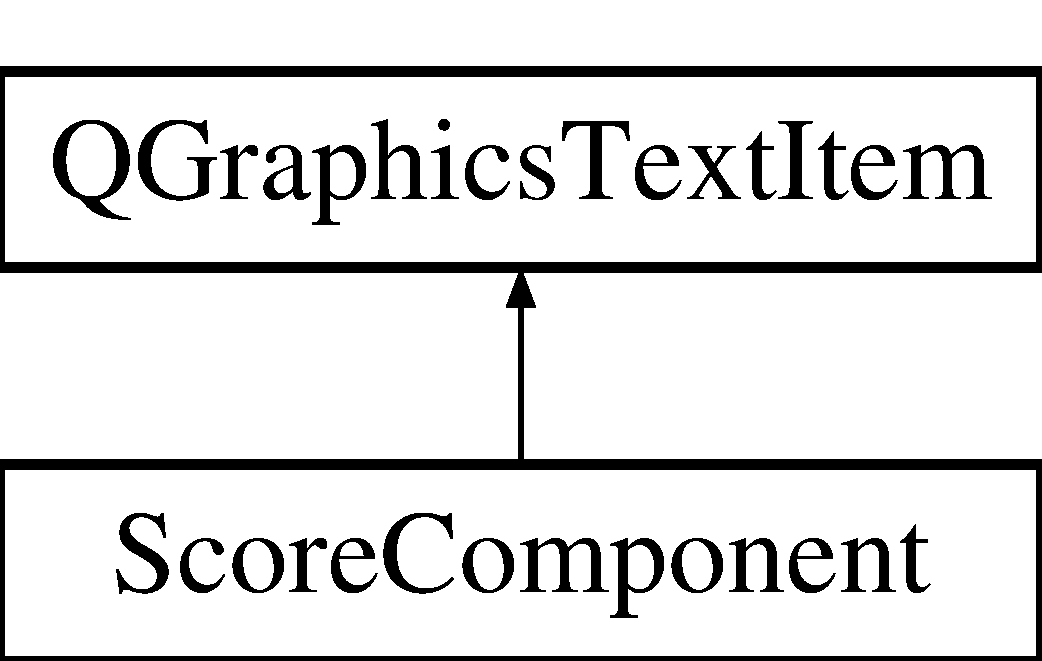
\includegraphics[height=2.000000cm]{classScoreComponent}
\end{center}
\end{figure}
\subsection*{Public Member Functions}
\begin{DoxyCompactItemize}
\item 
int \hyperlink{classScoreComponent_ac6ea09da203a3fa8424f4c0201629148}{getscore\-Display\-Diff\-X} ()
\begin{DoxyCompactList}\small\item\em Function to get score\-Display\-Diff\-X. \end{DoxyCompactList}\item 
int \hyperlink{classScoreComponent_a094c0593268e53b082f18a74a7774890}{getscore\-Display\-Diff\-Y} ()
\begin{DoxyCompactList}\small\item\em Function to get score\-Display\-Diff\-Y. \end{DoxyCompactList}\item 
\hyperlink{classScoreComponent_a39001d5cd9b6a7315d4bc9c9cf1b1383}{Score\-Component} (Q\-Graphics\-Scene $\ast$scene, qreal x\-\_\-coordinate, qreal y\-\_\-coordinate, int score\-\_\-display\-\_\-diff\-\_\-x, int score\-\_\-display\-\_\-diff\-\_\-y, Q\-Color text\-\_\-color, Q\-Font text\-\_\-font)
\begin{DoxyCompactList}\small\item\em Contructor. \end{DoxyCompactList}\item 
void \hyperlink{classScoreComponent_aa1d8f83108617d4e68209e480fb9964a}{update} (int new\-\_\-score)
\begin{DoxyCompactList}\small\item\em To Update \hyperlink{classScoreComponent}{Score\-Component}. \end{DoxyCompactList}\end{DoxyCompactItemize}
\subsection*{Public Attributes}
\begin{DoxyCompactItemize}
\item 
\hypertarget{classScoreComponent_af4e35536cd51f75d1eef5670ca914785}{const int \hyperlink{classScoreComponent_af4e35536cd51f75d1eef5670ca914785}{score\-Display\-Diff\-X}}\label{classScoreComponent_af4e35536cd51f75d1eef5670ca914785}

\begin{DoxyCompactList}\small\item\em X Coordinate of the Score Display. \end{DoxyCompactList}\item 
\hypertarget{classScoreComponent_a02fb0e04e19e4164ecec6a0e372ad06e}{const int \hyperlink{classScoreComponent_a02fb0e04e19e4164ecec6a0e372ad06e}{score\-Display\-Diff\-Y}}\label{classScoreComponent_a02fb0e04e19e4164ecec6a0e372ad06e}

\begin{DoxyCompactList}\small\item\em Y Coordinate of the Score Display. \end{DoxyCompactList}\end{DoxyCompactItemize}


\subsection{Detailed Description}
Class to Display the Score on top of Player. 

\subsection{Constructor \& Destructor Documentation}
\hypertarget{classScoreComponent_a39001d5cd9b6a7315d4bc9c9cf1b1383}{\index{Score\-Component@{Score\-Component}!Score\-Component@{Score\-Component}}
\index{Score\-Component@{Score\-Component}!ScoreComponent@{Score\-Component}}
\subsubsection[{Score\-Component}]{\setlength{\rightskip}{0pt plus 5cm}Score\-Component\-::\-Score\-Component (
\begin{DoxyParamCaption}
\item[{Q\-Graphics\-Scene $\ast$}]{scene, }
\item[{qreal}]{x\-\_\-coordinate, }
\item[{qreal}]{y\-\_\-coordinate, }
\item[{int}]{score\-\_\-display\-\_\-diff\-\_\-x, }
\item[{int}]{score\-\_\-display\-\_\-diff\-\_\-y, }
\item[{Q\-Color}]{text\-\_\-color, }
\item[{Q\-Font}]{text\-\_\-font}
\end{DoxyParamCaption}
)}}\label{classScoreComponent_a39001d5cd9b6a7315d4bc9c9cf1b1383}


Contructor. 


\begin{DoxyParams}{Parameters}
{\em scene} & The scene where to add the score component \\
\hline
{\em x\-\_\-coordinate} & the position of x coordinate \\
\hline
{\em y\-\_\-coordinate} & the position of y coordinate \\
\hline
{\em score\-\_\-display\-\_\-diff\-\_\-x} & Difference in player and Score position in X \\
\hline
{\em score\-\_\-display\-\_\-diff\-\_\-y} & Difference in player and Score position in Y \\
\hline
{\em text\-\_\-color} & Color of the \hyperlink{classScoreComponent}{Score\-Component} \\
\hline
{\em text\-\_\-font} & Font of the \hyperlink{classScoreComponent}{Score\-Component} \\
\hline
\end{DoxyParams}


\subsection{Member Function Documentation}
\hypertarget{classScoreComponent_ac6ea09da203a3fa8424f4c0201629148}{\index{Score\-Component@{Score\-Component}!getscore\-Display\-Diff\-X@{getscore\-Display\-Diff\-X}}
\index{getscore\-Display\-Diff\-X@{getscore\-Display\-Diff\-X}!ScoreComponent@{Score\-Component}}
\subsubsection[{getscore\-Display\-Diff\-X}]{\setlength{\rightskip}{0pt plus 5cm}int Score\-Component\-::getscore\-Display\-Diff\-X (
\begin{DoxyParamCaption}
{}
\end{DoxyParamCaption}
)}}\label{classScoreComponent_ac6ea09da203a3fa8424f4c0201629148}


Function to get score\-Display\-Diff\-X. 

\begin{DoxyReturn}{Returns}
value of score\-Display\-Diff\-X 
\end{DoxyReturn}
\hypertarget{classScoreComponent_a094c0593268e53b082f18a74a7774890}{\index{Score\-Component@{Score\-Component}!getscore\-Display\-Diff\-Y@{getscore\-Display\-Diff\-Y}}
\index{getscore\-Display\-Diff\-Y@{getscore\-Display\-Diff\-Y}!ScoreComponent@{Score\-Component}}
\subsubsection[{getscore\-Display\-Diff\-Y}]{\setlength{\rightskip}{0pt plus 5cm}int Score\-Component\-::getscore\-Display\-Diff\-Y (
\begin{DoxyParamCaption}
{}
\end{DoxyParamCaption}
)}}\label{classScoreComponent_a094c0593268e53b082f18a74a7774890}


Function to get score\-Display\-Diff\-Y. 

\begin{DoxyReturn}{Returns}
value of score\-Display\-Diff\-Y 
\end{DoxyReturn}
\hypertarget{classScoreComponent_aa1d8f83108617d4e68209e480fb9964a}{\index{Score\-Component@{Score\-Component}!update@{update}}
\index{update@{update}!ScoreComponent@{Score\-Component}}
\subsubsection[{update}]{\setlength{\rightskip}{0pt plus 5cm}void Score\-Component\-::update (
\begin{DoxyParamCaption}
\item[{int}]{new\-\_\-score}
\end{DoxyParamCaption}
)}}\label{classScoreComponent_aa1d8f83108617d4e68209e480fb9964a}


To Update \hyperlink{classScoreComponent}{Score\-Component}. 


\begin{DoxyParams}{Parameters}
{\em new\-\_\-score} & The new score \\
\hline
\end{DoxyParams}


The documentation for this class was generated from the following file\-:\begin{DoxyCompactItemize}
\item 
scorecomponent.\-h\end{DoxyCompactItemize}

\hypertarget{classServer}{\section{Server Class Reference}
\label{classServer}\index{Server@{Server}}
}


for making networking websocket server  




{\ttfamily \#include $<$server.\-h$>$}

Inheritance diagram for Server\-:\begin{figure}[H]
\begin{center}
\leavevmode
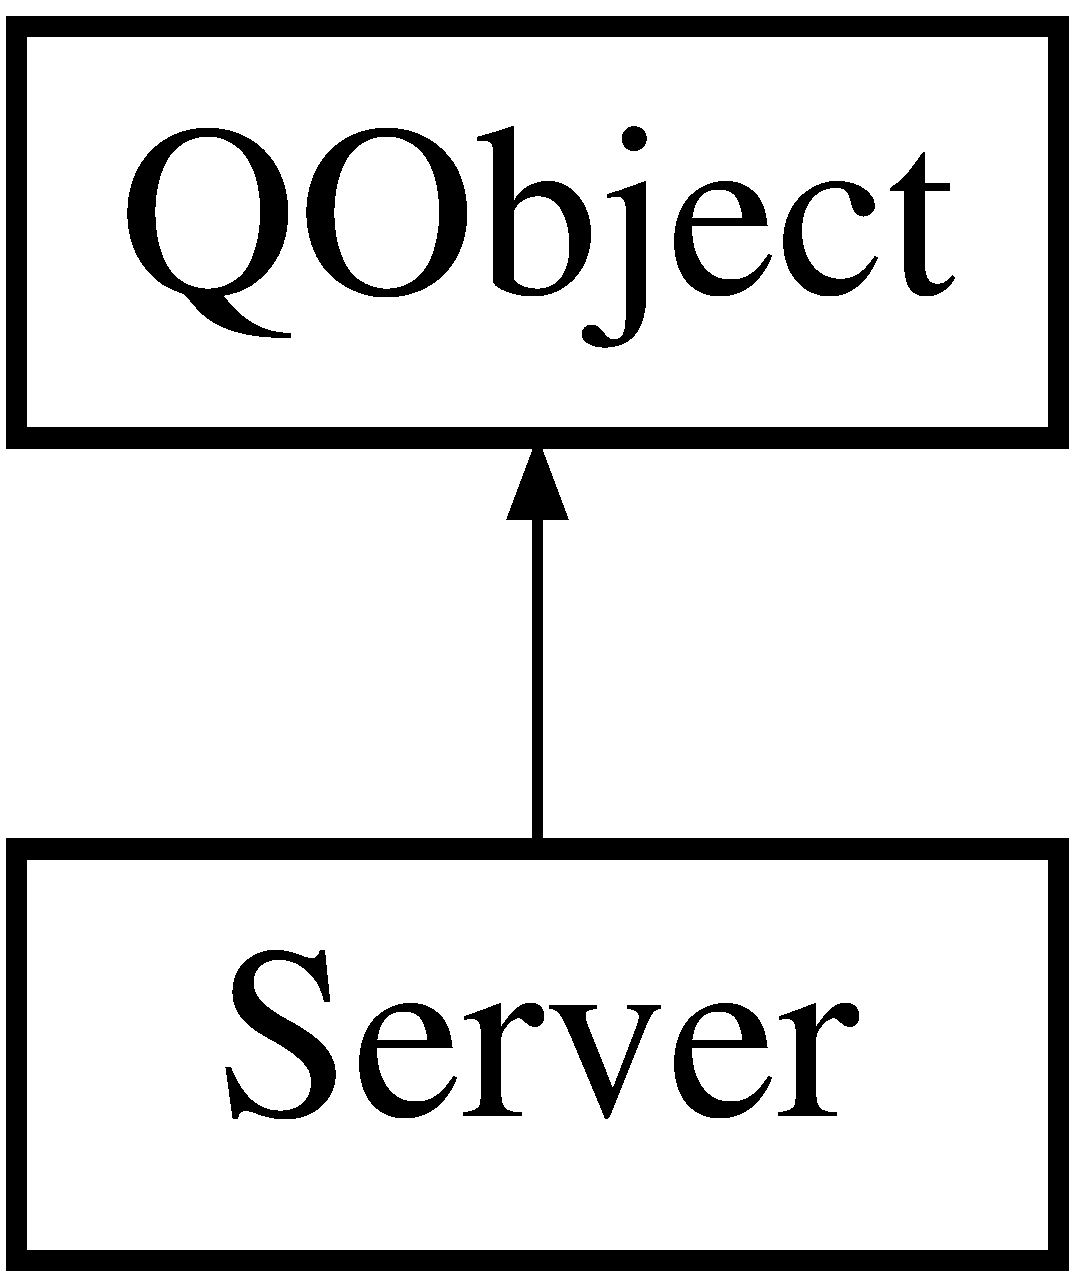
\includegraphics[height=2.000000cm]{classServer}
\end{center}
\end{figure}
\subsection*{Signals}
\begin{DoxyCompactItemize}
\item 
\hypertarget{classServer_a67295c05cd7776a05d4d26f3872b97d1}{void \hyperlink{classServer_a67295c05cd7776a05d4d26f3872b97d1}{closed} ()}\label{classServer_a67295c05cd7776a05d4d26f3872b97d1}

\begin{DoxyCompactList}\small\item\em signal to close screen \end{DoxyCompactList}\item 
\hypertarget{classServer_a064bb50dac3db0c39d99b512942251c7}{void \hyperlink{classServer_a064bb50dac3db0c39d99b512942251c7}{contents\-Changed} (Q\-String)}\label{classServer_a064bb50dac3db0c39d99b512942251c7}

\begin{DoxyCompactList}\small\item\em signal for changing content on screen \end{DoxyCompactList}\end{DoxyCompactItemize}
\subsection*{Public Member Functions}
\begin{DoxyCompactItemize}
\item 
\hypertarget{classServer_af5b47a498608d9cd1740621ae11172ca}{\hyperlink{classServer_af5b47a498608d9cd1740621ae11172ca}{Server} (quint16 port, Q\-Application $\ast$a, Q\-Graphics\-Scene $\ast$scene\-\_\-local, int milliseconds\-\_\-per\-\_\-frame, int number\-\_\-of\-\_\-threads, Q\-Label $\ast$label, Q\-Object $\ast$parent=N\-U\-L\-L)}\label{classServer_af5b47a498608d9cd1740621ae11172ca}

\begin{DoxyCompactList}\small\item\em constructor \end{DoxyCompactList}\item 
\hypertarget{classServer_a4b3aa2579cb1c8cd1d069582c14d0fa6}{\hyperlink{classServer_a4b3aa2579cb1c8cd1d069582c14d0fa6}{$\sim$\-Server} ()}\label{classServer_a4b3aa2579cb1c8cd1d069582c14d0fa6}

\begin{DoxyCompactList}\small\item\em destructor \end{DoxyCompactList}\item 
void \hyperlink{classServer_a21f4d5fa308381bd91b5d584b222c471}{start\-Server} (int screen\-\_\-width, int screen\-\_\-height)
\begin{DoxyCompactList}\small\item\em button click \end{DoxyCompactList}\item 
void \hyperlink{classServer_a4f7a988666f3cd4b91d14a6016a0cedf}{set\-Client\-I\-P\-List} (Q\-Graphics\-Text\-Item $\ast$client\-\_\-\-I\-P\-\_\-list)
\begin{DoxyCompactList}\small\item\em display no of connection \end{DoxyCompactList}\item 
\hypertarget{classServer_a5fa376b713c9c80ad1cd6ffb3ac1e23d}{void \hyperlink{classServer_a5fa376b713c9c80ad1cd6ffb3ac1e23d}{start\-Game\-Slot\-Button\-Click} (Q\-Graphics\-Text\-Item $\ast$server\-\_\-message)}\label{classServer_a5fa376b713c9c80ad1cd6ffb3ac1e23d}

\begin{DoxyCompactList}\small\item\em button click \end{DoxyCompactList}\end{DoxyCompactItemize}
\subsection*{Public Attributes}
\begin{DoxyCompactItemize}
\item 
\hypertarget{classServer_afff26cb9a4bb0c136ead3e974c725902}{\hyperlink{classGameState}{Game\-State} $\ast$ \hyperlink{classServer_afff26cb9a4bb0c136ead3e974c725902}{game\-Pointer}}\label{classServer_afff26cb9a4bb0c136ead3e974c725902}

\begin{DoxyCompactList}\small\item\em gamestate pointer \end{DoxyCompactList}\end{DoxyCompactItemize}


\subsection{Detailed Description}
for making networking websocket server 

\subsection{Member Function Documentation}
\hypertarget{classServer_a4f7a988666f3cd4b91d14a6016a0cedf}{\index{Server@{Server}!set\-Client\-I\-P\-List@{set\-Client\-I\-P\-List}}
\index{set\-Client\-I\-P\-List@{set\-Client\-I\-P\-List}!Server@{Server}}
\subsubsection[{set\-Client\-I\-P\-List}]{\setlength{\rightskip}{0pt plus 5cm}void Server\-::set\-Client\-I\-P\-List (
\begin{DoxyParamCaption}
\item[{Q\-Graphics\-Text\-Item $\ast$}]{client\-\_\-\-I\-P\-\_\-list}
\end{DoxyParamCaption}
)}}\label{classServer_a4f7a988666f3cd4b91d14a6016a0cedf}


display no of connection 


\begin{DoxyParams}{Parameters}
{\em client\-\_\-\-I\-P\-\_\-list} & text\-Item pointer \\
\hline
\end{DoxyParams}
\hypertarget{classServer_a21f4d5fa308381bd91b5d584b222c471}{\index{Server@{Server}!start\-Server@{start\-Server}}
\index{start\-Server@{start\-Server}!Server@{Server}}
\subsubsection[{start\-Server}]{\setlength{\rightskip}{0pt plus 5cm}void Server\-::start\-Server (
\begin{DoxyParamCaption}
\item[{int}]{screen\-\_\-width, }
\item[{int}]{screen\-\_\-height}
\end{DoxyParamCaption}
)}}\label{classServer_a21f4d5fa308381bd91b5d584b222c471}


button click 


\begin{DoxyParams}{Parameters}
{\em screen} & width \\
\hline
{\em screen} & height \\
\hline
\end{DoxyParams}


The documentation for this class was generated from the following file\-:\begin{DoxyCompactItemize}
\item 
server.\-h\end{DoxyCompactItemize}

\hypertarget{classState}{\section{State Class Reference}
\label{classState}\index{State@{State}}
}


Class to Identify the Different States that the Players can be in.  




{\ttfamily \#include $<$state.\-h$>$}

Inheritance diagram for State\-:\begin{figure}[H]
\begin{center}
\leavevmode
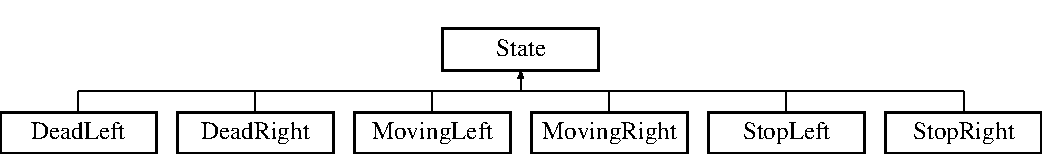
\includegraphics[height=2.000000cm]{classState}
\end{center}
\end{figure}
\subsection*{Public Member Functions}
\begin{DoxyCompactItemize}
\item 
\hypertarget{classState_a9ddc1df6f998184d6477b48fab90281c}{virtual \hyperlink{classState_a9ddc1df6f998184d6477b48fab90281c}{$\sim$\-State} ()}\label{classState_a9ddc1df6f998184d6477b48fab90281c}

\begin{DoxyCompactList}\small\item\em Destructor. \end{DoxyCompactList}\item 
virtual \hyperlink{classState}{State} $\ast$ \hyperlink{classState_a5f2bc9804614c5ca9e7feb7d8c57668d}{update} (\hyperlink{classInputComponent}{Input\-Component} $\ast$, std\-::set$<$ Qt\-::\-Key $>$)=0
\begin{DoxyCompactList}\small\item\em Virtual Fucntion to update the current state based on keypressevent. \end{DoxyCompactList}\item 
virtual \hyperlink{namespaceenumerator_a5fc7b342c2c633e1037b07cea237a222}{enumerator\-::\-State} \hyperlink{classState_a8c6cc1ff1ecdf88e586f857339b7e071}{type} ()=0
\begin{DoxyCompactList}\small\item\em Provides the Type of \hyperlink{classState}{State}. \end{DoxyCompactList}\end{DoxyCompactItemize}


\subsection{Detailed Description}
Class to Identify the Different States that the Players can be in. 

\subsection{Member Function Documentation}
\hypertarget{classState_a8c6cc1ff1ecdf88e586f857339b7e071}{\index{State@{State}!type@{type}}
\index{type@{type}!State@{State}}
\subsubsection[{type}]{\setlength{\rightskip}{0pt plus 5cm}virtual {\bf enumerator\-::\-State} State\-::type (
\begin{DoxyParamCaption}
{}
\end{DoxyParamCaption}
)\hspace{0.3cm}{\ttfamily [pure virtual]}}}\label{classState_a8c6cc1ff1ecdf88e586f857339b7e071}


Provides the Type of \hyperlink{classState}{State}. 

\begin{DoxyReturn}{Returns}
enumerator\-::\-State\-::\-S\-T\-A\-T\-E\-\_\-\-T\-Y\-P\-E 
\end{DoxyReturn}


Implemented in \hyperlink{classMovingLeft_a2bf0f28568b5188d4b9bad622b52e47d}{Moving\-Left}, \hyperlink{classMovingRight_a9d8e60b64a11346a518e222ae36366ca}{Moving\-Right}, \hyperlink{classDeadLeft_a564f47ceebef43f5553072c446b3c12f}{Dead\-Left}, \hyperlink{classDeadRight_abd8e52205ddafd19858a81f25cd87106}{Dead\-Right}, \hyperlink{classStopLeft_a715c78b6093aa8624c41582c2435ee69}{Stop\-Left}, and \hyperlink{classStopRight_a5d5dabb814633abfb33d114806be282a}{Stop\-Right}.

\hypertarget{classState_a5f2bc9804614c5ca9e7feb7d8c57668d}{\index{State@{State}!update@{update}}
\index{update@{update}!State@{State}}
\subsubsection[{update}]{\setlength{\rightskip}{0pt plus 5cm}virtual {\bf State}$\ast$ State\-::update (
\begin{DoxyParamCaption}
\item[{{\bf Input\-Component} $\ast$}]{, }
\item[{std\-::set$<$ Qt\-::\-Key $>$}]{}
\end{DoxyParamCaption}
)\hspace{0.3cm}{\ttfamily [pure virtual]}}}\label{classState_a5f2bc9804614c5ca9e7feb7d8c57668d}


Virtual Fucntion to update the current state based on keypressevent. 

\begin{DoxyReturn}{Returns}

\end{DoxyReturn}


Implemented in \hyperlink{classMovingLeft_a0ddbc7a065b820e06caa76c650ab6765}{Moving\-Left}, \hyperlink{classMovingRight_aa3ccaf974ea8137e77a26cb3738345c1}{Moving\-Right}, \hyperlink{classDeadLeft_a641116efda392a1c6437e9034443a1ea}{Dead\-Left}, \hyperlink{classDeadRight_a90bbfab63b08a87dd2b36bbdb8830aa5}{Dead\-Right}, \hyperlink{classStopLeft_ae853fc7d82f2a8d306adc186ab9e52dd}{Stop\-Left}, and \hyperlink{classStopRight_a40403908f1cf3ac8ca809c550fea3783}{Stop\-Right}.



The documentation for this class was generated from the following file\-:\begin{DoxyCompactItemize}
\item 
state.\-h\end{DoxyCompactItemize}

\hypertarget{classStopLeft}{\section{Stop\-Left Class Reference}
\label{classStopLeft}\index{Stop\-Left@{Stop\-Left}}
}


The state in which the player is standing facing left This also handles the responds to key press and key release inputs so as to change the state of the \hyperlink{classGameObject}{Game\-Object}.  




{\ttfamily \#include $<$stopleft.\-h$>$}

Inheritance diagram for Stop\-Left\-:\begin{figure}[H]
\begin{center}
\leavevmode
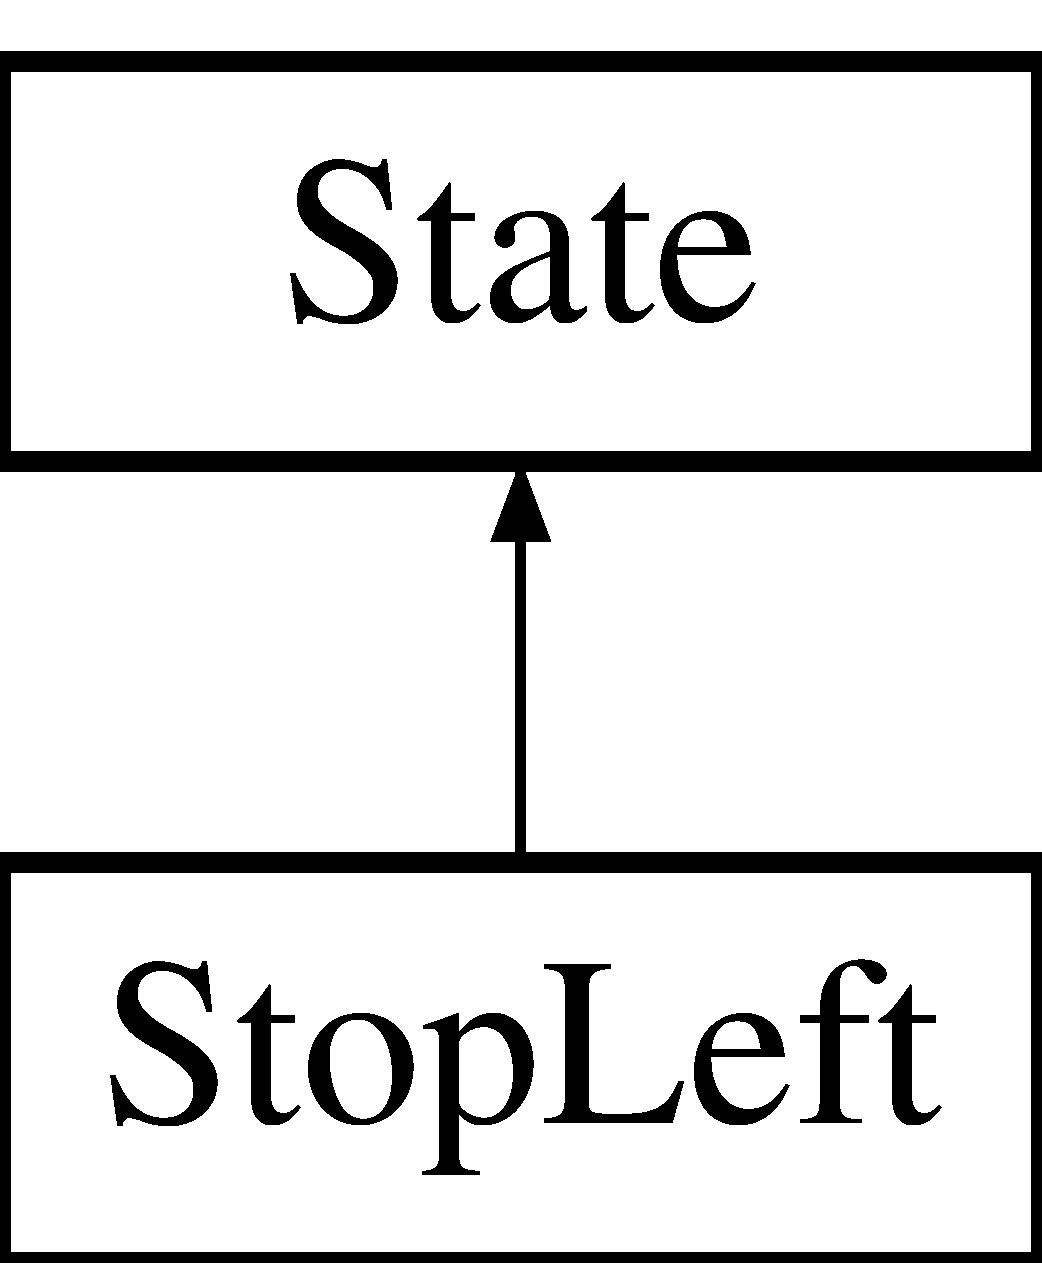
\includegraphics[height=2.000000cm]{classStopLeft}
\end{center}
\end{figure}
\subsection*{Public Member Functions}
\begin{DoxyCompactItemize}
\item 
\hypertarget{classStopLeft_ae09316bd4da3643256b6b7d464117a58}{virtual \hyperlink{classStopLeft_ae09316bd4da3643256b6b7d464117a58}{$\sim$\-Stop\-Left} ()}\label{classStopLeft_ae09316bd4da3643256b6b7d464117a58}

\begin{DoxyCompactList}\small\item\em Destructor. \end{DoxyCompactList}\item 
virtual \hyperlink{classState}{State} $\ast$ \hyperlink{classStopLeft_ae853fc7d82f2a8d306adc186ab9e52dd}{update} (\hyperlink{classInputComponent}{Input\-Component} $\ast$input\-Component, std\-::set$<$ Qt\-::\-Key $>$ key)
\begin{DoxyCompactList}\small\item\em Updates the state on the basis of the keys currently pressed. \end{DoxyCompactList}\item 
virtual \hyperlink{namespaceenumerator_a5fc7b342c2c633e1037b07cea237a222}{enumerator\-::\-State} \hyperlink{classStopLeft_a715c78b6093aa8624c41582c2435ee69}{type} ()
\begin{DoxyCompactList}\small\item\em Provides the type of the \hyperlink{classState}{State}. \end{DoxyCompactList}\end{DoxyCompactItemize}


\subsection{Detailed Description}
The state in which the player is standing facing left This also handles the responds to key press and key release inputs so as to change the state of the \hyperlink{classGameObject}{Game\-Object}. 

\subsection{Member Function Documentation}
\hypertarget{classStopLeft_a715c78b6093aa8624c41582c2435ee69}{\index{Stop\-Left@{Stop\-Left}!type@{type}}
\index{type@{type}!StopLeft@{Stop\-Left}}
\subsubsection[{type}]{\setlength{\rightskip}{0pt plus 5cm}virtual {\bf enumerator\-::\-State} Stop\-Left\-::type (
\begin{DoxyParamCaption}
{}
\end{DoxyParamCaption}
)\hspace{0.3cm}{\ttfamily [virtual]}}}\label{classStopLeft_a715c78b6093aa8624c41582c2435ee69}


Provides the type of the \hyperlink{classState}{State}. 

\begin{DoxyReturn}{Returns}
enumerator\-::\-State\-::\-S\-T\-O\-P\-\_\-\-L\-E\-F\-T 
\end{DoxyReturn}


Implements \hyperlink{classState_a8c6cc1ff1ecdf88e586f857339b7e071}{State}.

\hypertarget{classStopLeft_ae853fc7d82f2a8d306adc186ab9e52dd}{\index{Stop\-Left@{Stop\-Left}!update@{update}}
\index{update@{update}!StopLeft@{Stop\-Left}}
\subsubsection[{update}]{\setlength{\rightskip}{0pt plus 5cm}virtual {\bf State}$\ast$ Stop\-Left\-::update (
\begin{DoxyParamCaption}
\item[{{\bf Input\-Component} $\ast$}]{input\-Component, }
\item[{std\-::set$<$ Qt\-::\-Key $>$}]{key}
\end{DoxyParamCaption}
)\hspace{0.3cm}{\ttfamily [virtual]}}}\label{classStopLeft_ae853fc7d82f2a8d306adc186ab9e52dd}


Updates the state on the basis of the keys currently pressed. 


\begin{DoxyParams}{Parameters}
{\em input\-Component} & the \hyperlink{classInputComponent}{Input\-Component} of the \hyperlink{classGameObject}{Game\-Object} whose state is being updated \\
\hline
{\em key} & the set of keys currently pressed \\
\hline
\end{DoxyParams}
\begin{DoxyReturn}{Returns}
the new state 
\end{DoxyReturn}


Implements \hyperlink{classState_a5f2bc9804614c5ca9e7feb7d8c57668d}{State}.



The documentation for this class was generated from the following file\-:\begin{DoxyCompactItemize}
\item 
stopleft.\-h\end{DoxyCompactItemize}

\hypertarget{classStopRight}{\section{Stop\-Right Class Reference}
\label{classStopRight}\index{Stop\-Right@{Stop\-Right}}
}


The state in which the player is standing facing right This also handles the responds to key press and key release inputs so as to change the state of the \hyperlink{classGameObject}{Game\-Object}.  




{\ttfamily \#include $<$stopright.\-h$>$}

Inheritance diagram for Stop\-Right\-:\begin{figure}[H]
\begin{center}
\leavevmode
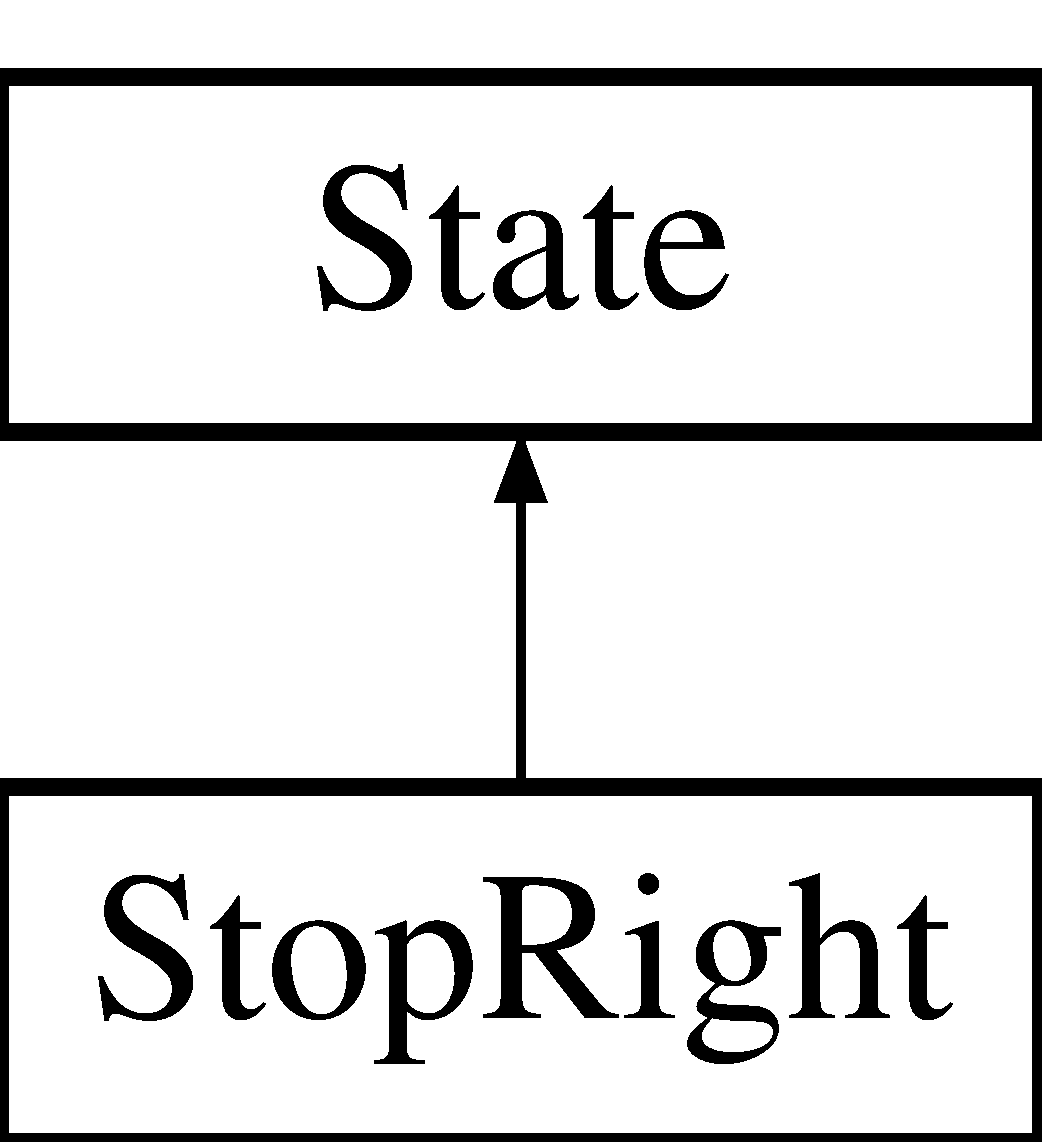
\includegraphics[height=2.000000cm]{classStopRight}
\end{center}
\end{figure}
\subsection*{Public Member Functions}
\begin{DoxyCompactItemize}
\item 
\hypertarget{classStopRight_a545fb26595a15ade51344e4ec7837aaf}{virtual \hyperlink{classStopRight_a545fb26595a15ade51344e4ec7837aaf}{$\sim$\-Stop\-Right} ()}\label{classStopRight_a545fb26595a15ade51344e4ec7837aaf}

\begin{DoxyCompactList}\small\item\em Destructor. \end{DoxyCompactList}\item 
virtual \hyperlink{classState}{State} $\ast$ \hyperlink{classStopRight_a40403908f1cf3ac8ca809c550fea3783}{update} (\hyperlink{classInputComponent}{Input\-Component} $\ast$input\-Component, std\-::set$<$ Qt\-::\-Key $>$ key)
\begin{DoxyCompactList}\small\item\em Updates the state on the basis of the keys currently pressed. \end{DoxyCompactList}\item 
virtual \hyperlink{namespaceenumerator_a5fc7b342c2c633e1037b07cea237a222}{enumerator\-::\-State} \hyperlink{classStopRight_a5d5dabb814633abfb33d114806be282a}{type} ()
\begin{DoxyCompactList}\small\item\em Provides the type of the \hyperlink{classState}{State}. \end{DoxyCompactList}\end{DoxyCompactItemize}


\subsection{Detailed Description}
The state in which the player is standing facing right This also handles the responds to key press and key release inputs so as to change the state of the \hyperlink{classGameObject}{Game\-Object}. 

\subsection{Member Function Documentation}
\hypertarget{classStopRight_a5d5dabb814633abfb33d114806be282a}{\index{Stop\-Right@{Stop\-Right}!type@{type}}
\index{type@{type}!StopRight@{Stop\-Right}}
\subsubsection[{type}]{\setlength{\rightskip}{0pt plus 5cm}virtual {\bf enumerator\-::\-State} Stop\-Right\-::type (
\begin{DoxyParamCaption}
{}
\end{DoxyParamCaption}
)\hspace{0.3cm}{\ttfamily [virtual]}}}\label{classStopRight_a5d5dabb814633abfb33d114806be282a}


Provides the type of the \hyperlink{classState}{State}. 

\begin{DoxyReturn}{Returns}
enumerator\-::\-State\-::\-S\-T\-O\-P\-\_\-\-R\-I\-G\-H\-T 
\end{DoxyReturn}


Implements \hyperlink{classState_a8c6cc1ff1ecdf88e586f857339b7e071}{State}.

\hypertarget{classStopRight_a40403908f1cf3ac8ca809c550fea3783}{\index{Stop\-Right@{Stop\-Right}!update@{update}}
\index{update@{update}!StopRight@{Stop\-Right}}
\subsubsection[{update}]{\setlength{\rightskip}{0pt plus 5cm}virtual {\bf State}$\ast$ Stop\-Right\-::update (
\begin{DoxyParamCaption}
\item[{{\bf Input\-Component} $\ast$}]{input\-Component, }
\item[{std\-::set$<$ Qt\-::\-Key $>$}]{key}
\end{DoxyParamCaption}
)\hspace{0.3cm}{\ttfamily [virtual]}}}\label{classStopRight_a40403908f1cf3ac8ca809c550fea3783}


Updates the state on the basis of the keys currently pressed. 


\begin{DoxyParams}{Parameters}
{\em input\-Component} & the \hyperlink{classInputComponent}{Input\-Component} of the \hyperlink{classGameObject}{Game\-Object} whose state is being updated \\
\hline
{\em key} & the set of keys currently pressed \\
\hline
\end{DoxyParams}
\begin{DoxyReturn}{Returns}
the new state 
\end{DoxyReturn}


Implements \hyperlink{classState_a5f2bc9804614c5ca9e7feb7d8c57668d}{State}.



The documentation for this class was generated from the following file\-:\begin{DoxyCompactItemize}
\item 
stopright.\-h\end{DoxyCompactItemize}

\hypertarget{classThreadPool}{\section{Thread\-Pool Class Reference}
\label{classThreadPool}\index{Thread\-Pool@{Thread\-Pool}}
}


Thread Pool to allot work concurrently Handles the creation of threads, assigns work, and handles wait till all threads complete execution.  




{\ttfamily \#include $<$threadpool.\-h$>$}

\subsection*{Public Member Functions}
\begin{DoxyCompactItemize}
\item 
\hyperlink{classThreadPool_a53fb4db20e08699bb52c2c332f611cc9}{Thread\-Pool} (int number\-\_\-of\-\_\-threads)
\begin{DoxyCompactList}\small\item\em Constructor. \end{DoxyCompactList}\item 
\hypertarget{classThreadPool_a7290a593e893111e2db6a6e226c471cb}{void \hyperlink{classThreadPool_a7290a593e893111e2db6a6e226c471cb}{add\-Thread} ()}\label{classThreadPool_a7290a593e893111e2db6a6e226c471cb}

\begin{DoxyCompactList}\small\item\em Adds a thread to the thread pool. \end{DoxyCompactList}\item 
void \hyperlink{classThreadPool_a07a236b214390a314589c1432d091d38}{assign\-To\-Thread} (std\-::function$<$ void()$>$ function\-\_\-to\-\_\-execute)
\begin{DoxyCompactList}\small\item\em Puts function in the queue waiting for a thread to execute. \end{DoxyCompactList}\item 
void \hyperlink{classThreadPool_a29dd5bbafbf80aeb33a1f60de36baed4}{wait\-Or\-Work} (int i)
\begin{DoxyCompactList}\small\item\em function run by each thread that waits till work is available in the queue, and executes it \end{DoxyCompactList}\item 
\hypertarget{classThreadPool_a44d3d2ab618970605e684efc216655eb}{\hyperlink{classThreadPool_a44d3d2ab618970605e684efc216655eb}{$\sim$\-Thread\-Pool} ()}\label{classThreadPool_a44d3d2ab618970605e684efc216655eb}

\begin{DoxyCompactList}\small\item\em Destructor. \end{DoxyCompactList}\item 
\hypertarget{classThreadPool_ac6f5b38e46d7c1225f726c2c2d3fa02e}{void \hyperlink{classThreadPool_ac6f5b38e46d7c1225f726c2c2d3fa02e}{wait\-Till\-All\-Complete} ()}\label{classThreadPool_ac6f5b38e46d7c1225f726c2c2d3fa02e}

\begin{DoxyCompactList}\small\item\em Wait till all current threads complete their current tasks. \end{DoxyCompactList}\end{DoxyCompactItemize}


\subsection{Detailed Description}
Thread Pool to allot work concurrently Handles the creation of threads, assigns work, and handles wait till all threads complete execution. 

\subsection{Constructor \& Destructor Documentation}
\hypertarget{classThreadPool_a53fb4db20e08699bb52c2c332f611cc9}{\index{Thread\-Pool@{Thread\-Pool}!Thread\-Pool@{Thread\-Pool}}
\index{Thread\-Pool@{Thread\-Pool}!ThreadPool@{Thread\-Pool}}
\subsubsection[{Thread\-Pool}]{\setlength{\rightskip}{0pt plus 5cm}Thread\-Pool\-::\-Thread\-Pool (
\begin{DoxyParamCaption}
\item[{int}]{number\-\_\-of\-\_\-threads}
\end{DoxyParamCaption}
)}}\label{classThreadPool_a53fb4db20e08699bb52c2c332f611cc9}


Constructor. 


\begin{DoxyParams}{Parameters}
{\em number\-\_\-of\-\_\-threads} & the number of threads in the thread pool \\
\hline
\end{DoxyParams}


\subsection{Member Function Documentation}
\hypertarget{classThreadPool_a07a236b214390a314589c1432d091d38}{\index{Thread\-Pool@{Thread\-Pool}!assign\-To\-Thread@{assign\-To\-Thread}}
\index{assign\-To\-Thread@{assign\-To\-Thread}!ThreadPool@{Thread\-Pool}}
\subsubsection[{assign\-To\-Thread}]{\setlength{\rightskip}{0pt plus 5cm}void Thread\-Pool\-::assign\-To\-Thread (
\begin{DoxyParamCaption}
\item[{std\-::function$<$ void()$>$}]{function\-\_\-to\-\_\-execute}
\end{DoxyParamCaption}
)}}\label{classThreadPool_a07a236b214390a314589c1432d091d38}


Puts function in the queue waiting for a thread to execute. 


\begin{DoxyParams}{Parameters}
{\em function\-\_\-to\-\_\-execute} & the function to be executed \\
\hline
\end{DoxyParams}
\hypertarget{classThreadPool_a29dd5bbafbf80aeb33a1f60de36baed4}{\index{Thread\-Pool@{Thread\-Pool}!wait\-Or\-Work@{wait\-Or\-Work}}
\index{wait\-Or\-Work@{wait\-Or\-Work}!ThreadPool@{Thread\-Pool}}
\subsubsection[{wait\-Or\-Work}]{\setlength{\rightskip}{0pt plus 5cm}void Thread\-Pool\-::wait\-Or\-Work (
\begin{DoxyParamCaption}
\item[{int}]{i}
\end{DoxyParamCaption}
)}}\label{classThreadPool_a29dd5bbafbf80aeb33a1f60de36baed4}


function run by each thread that waits till work is available in the queue, and executes it 


\begin{DoxyParams}{Parameters}
{\em i} & the I\-D of the thread \\
\hline
\end{DoxyParams}


The documentation for this class was generated from the following file\-:\begin{DoxyCompactItemize}
\item 
threadpool.\-h\end{DoxyCompactItemize}

\hypertarget{classTile}{\section{Tile Class Reference}
\label{classTile}\index{Tile@{Tile}}
}


The Class to Make Tiles A class for a tile rectangle Used for stopping player on obstacle detection.  




{\ttfamily \#include $<$tile.\-h$>$}

Inheritance diagram for Tile\-:\begin{figure}[H]
\begin{center}
\leavevmode
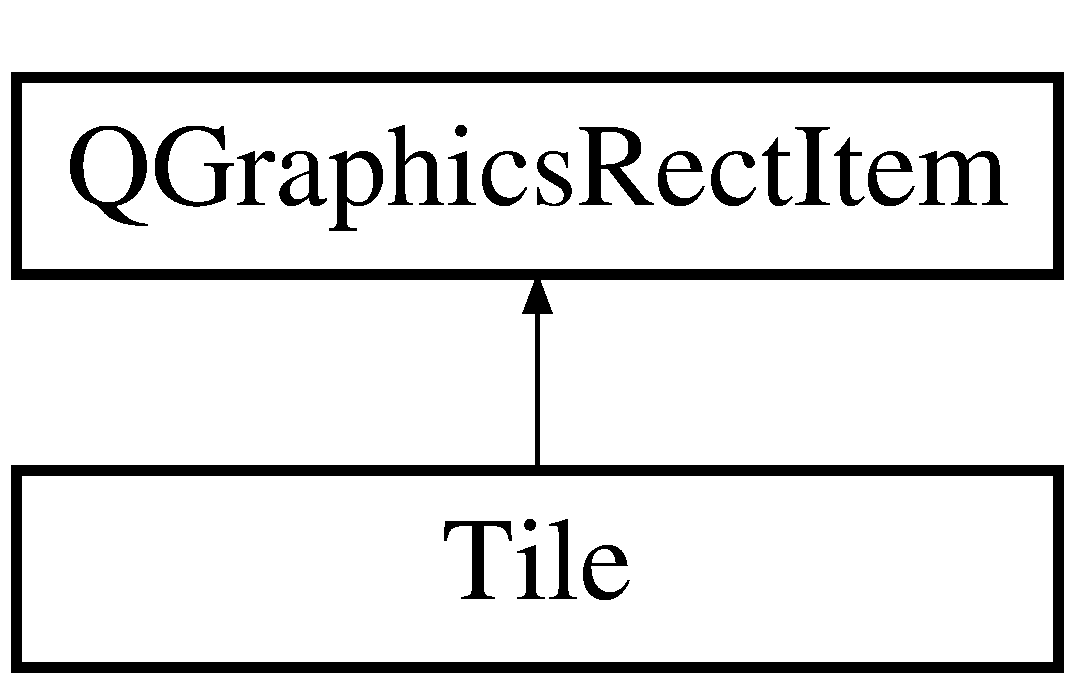
\includegraphics[height=2.000000cm]{classTile}
\end{center}
\end{figure}
\subsection*{Public Member Functions}
\begin{DoxyCompactItemize}
\item 
\hyperlink{classTile_a0c8a68113931418daaefdb0b868de535}{Tile} (Q\-Graphics\-Scene $\ast$scene, qreal column, qreal row, qreal width, qreal height, bool is\-\_\-obstacle)
\begin{DoxyCompactList}\small\item\em Constructor For \hyperlink{classTile}{Tile} Class. \end{DoxyCompactList}\item 
Q\-Graphics\-Rect\-Item $\ast$ \hyperlink{classTile_a5f75e3b66eb0770ce484fd3a29ba5d02}{get\-R} ()
\begin{DoxyCompactList}\small\item\em Function to get the pointer to the \hyperlink{classTile}{Tile}. \end{DoxyCompactList}\item 
bool \hyperlink{classTile_af7ad6e5f284e0888004d06ace947e9ae}{get\-Is\-Obstacle} ()
\begin{DoxyCompactList}\small\item\em Function to check if it's obstacle. \end{DoxyCompactList}\item 
qreal \hyperlink{classTile_a6e0d374fddc0462cb7f18ea06bd1ea92}{get\-Width\-Of\-Tile} ()
\begin{DoxyCompactList}\small\item\em Function to return width of \hyperlink{classTile}{Tile}. \end{DoxyCompactList}\item 
qreal \hyperlink{classTile_a785e906801dfd6a3bf9d5538bb2ed51e}{get\-Height\-Of\-Tile} ()
\begin{DoxyCompactList}\small\item\em Fucntion to return height of \hyperlink{classTile}{Tile}. \end{DoxyCompactList}\end{DoxyCompactItemize}


\subsection{Detailed Description}
The Class to Make Tiles A class for a tile rectangle Used for stopping player on obstacle detection. 

\subsection{Constructor \& Destructor Documentation}
\hypertarget{classTile_a0c8a68113931418daaefdb0b868de535}{\index{Tile@{Tile}!Tile@{Tile}}
\index{Tile@{Tile}!Tile@{Tile}}
\subsubsection[{Tile}]{\setlength{\rightskip}{0pt plus 5cm}Tile\-::\-Tile (
\begin{DoxyParamCaption}
\item[{Q\-Graphics\-Scene $\ast$}]{scene, }
\item[{qreal}]{column, }
\item[{qreal}]{row, }
\item[{qreal}]{width, }
\item[{qreal}]{height, }
\item[{bool}]{is\-\_\-obstacle}
\end{DoxyParamCaption}
)}}\label{classTile_a0c8a68113931418daaefdb0b868de535}


Constructor For \hyperlink{classTile}{Tile} Class. 


\begin{DoxyParams}{Parameters}
{\em scene} & The pointer to the Scene where to add the \hyperlink{classTile}{Tile} \\
\hline
{\em column} & The x Coordinate of The \hyperlink{classTile}{Tile} \\
\hline
{\em row} & The y Coordinate of the \hyperlink{classTile}{Tile} \\
\hline
{\em width} & Widthh of the \hyperlink{classTile}{Tile} \\
\hline
{\em height} & Width of the \hyperlink{classTile}{Tile} \\
\hline
{\em is\-\_\-obstacle} & To see if it's an obstacle \\
\hline
\end{DoxyParams}


\subsection{Member Function Documentation}
\hypertarget{classTile_a785e906801dfd6a3bf9d5538bb2ed51e}{\index{Tile@{Tile}!get\-Height\-Of\-Tile@{get\-Height\-Of\-Tile}}
\index{get\-Height\-Of\-Tile@{get\-Height\-Of\-Tile}!Tile@{Tile}}
\subsubsection[{get\-Height\-Of\-Tile}]{\setlength{\rightskip}{0pt plus 5cm}qreal Tile\-::get\-Height\-Of\-Tile (
\begin{DoxyParamCaption}
{}
\end{DoxyParamCaption}
)}}\label{classTile_a785e906801dfd6a3bf9d5538bb2ed51e}


Fucntion to return height of \hyperlink{classTile}{Tile}. 

\begin{DoxyReturn}{Returns}
Height of \hyperlink{classTile}{Tile} 
\end{DoxyReturn}
\hypertarget{classTile_af7ad6e5f284e0888004d06ace947e9ae}{\index{Tile@{Tile}!get\-Is\-Obstacle@{get\-Is\-Obstacle}}
\index{get\-Is\-Obstacle@{get\-Is\-Obstacle}!Tile@{Tile}}
\subsubsection[{get\-Is\-Obstacle}]{\setlength{\rightskip}{0pt plus 5cm}bool Tile\-::get\-Is\-Obstacle (
\begin{DoxyParamCaption}
{}
\end{DoxyParamCaption}
)}}\label{classTile_af7ad6e5f284e0888004d06ace947e9ae}


Function to check if it's obstacle. 

\begin{DoxyReturn}{Returns}
Returns the value of is\-Obstacle 
\end{DoxyReturn}
\hypertarget{classTile_a5f75e3b66eb0770ce484fd3a29ba5d02}{\index{Tile@{Tile}!get\-R@{get\-R}}
\index{get\-R@{get\-R}!Tile@{Tile}}
\subsubsection[{get\-R}]{\setlength{\rightskip}{0pt plus 5cm}Q\-Graphics\-Rect\-Item$\ast$ Tile\-::get\-R (
\begin{DoxyParamCaption}
{}
\end{DoxyParamCaption}
)}}\label{classTile_a5f75e3b66eb0770ce484fd3a29ba5d02}


Function to get the pointer to the \hyperlink{classTile}{Tile}. 

\begin{DoxyReturn}{Returns}
Returns the pointer to the \hyperlink{classTile}{Tile} 
\end{DoxyReturn}
\hypertarget{classTile_a6e0d374fddc0462cb7f18ea06bd1ea92}{\index{Tile@{Tile}!get\-Width\-Of\-Tile@{get\-Width\-Of\-Tile}}
\index{get\-Width\-Of\-Tile@{get\-Width\-Of\-Tile}!Tile@{Tile}}
\subsubsection[{get\-Width\-Of\-Tile}]{\setlength{\rightskip}{0pt plus 5cm}qreal Tile\-::get\-Width\-Of\-Tile (
\begin{DoxyParamCaption}
{}
\end{DoxyParamCaption}
)}}\label{classTile_a6e0d374fddc0462cb7f18ea06bd1ea92}


Function to return width of \hyperlink{classTile}{Tile}. 

\begin{DoxyReturn}{Returns}
Width of \hyperlink{classTile}{Tile} 
\end{DoxyReturn}


The documentation for this class was generated from the following file\-:\begin{DoxyCompactItemize}
\item 
tile.\-h\end{DoxyCompactItemize}

\hypertarget{classTimer}{\section{Timer Class Reference}
\label{classTimer}\index{Timer@{Timer}}
}


Class That maintains the timer.  




{\ttfamily \#include $<$timer.\-h$>$}

Inheritance diagram for Timer\-:\begin{figure}[H]
\begin{center}
\leavevmode
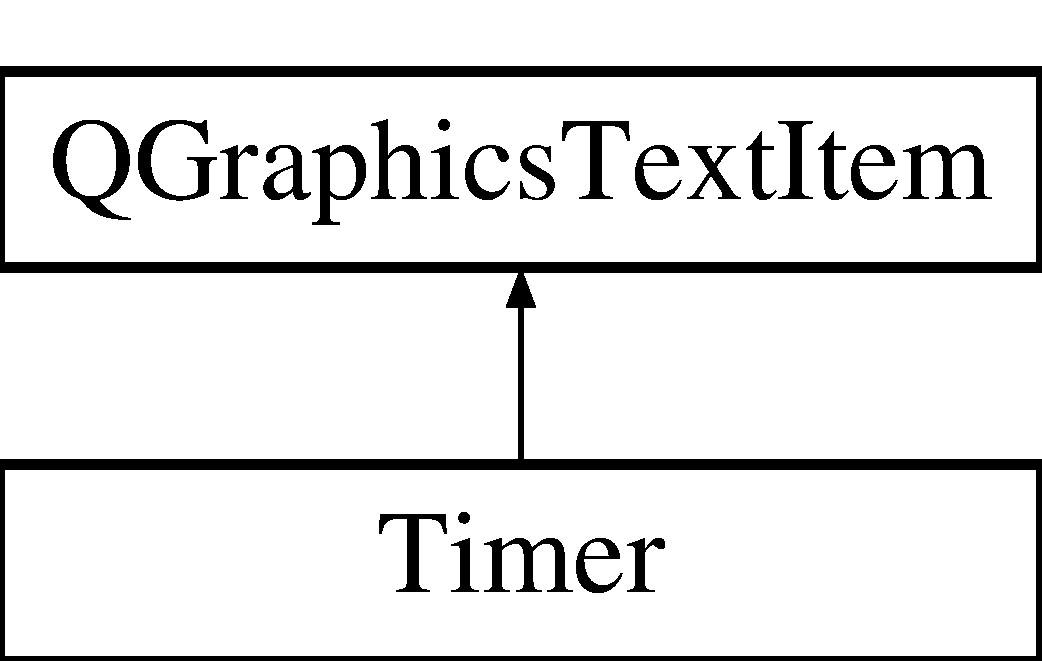
\includegraphics[height=2.000000cm]{classTimer}
\end{center}
\end{figure}
\subsection*{Public Member Functions}
\begin{DoxyCompactItemize}
\item 
\hyperlink{classTimer_a58988682da3ca1b076605faa4d97415f}{Timer} (int total\-\_\-time\-\_\-available, int milliseconds\-\_\-per\-\_\-frame)
\begin{DoxyCompactList}\small\item\em Constructor for \hyperlink{classTimer}{Timer} Class. \end{DoxyCompactList}\item 
\hypertarget{classTimer_ad3c95ce902fce977d280256256856d64}{virtual \hyperlink{classTimer_ad3c95ce902fce977d280256256856d64}{$\sim$\-Timer} ()}\label{classTimer_ad3c95ce902fce977d280256256856d64}

\begin{DoxyCompactList}\small\item\em Destructor for \hyperlink{classTimer}{Timer} Class. \end{DoxyCompactList}\item 
bool \hyperlink{classTimer_a953317a04cb8e28d24ef0f12220db90f}{is\-Time\-Left} ()
\begin{DoxyCompactList}\small\item\em To check if time is left. \end{DoxyCompactList}\item 
\hypertarget{classTimer_af4ace519cf8f0d4acd8de4ed261d43fb}{void \hyperlink{classTimer_af4ace519cf8f0d4acd8de4ed261d43fb}{update\-Timer\-On\-Screen} ()}\label{classTimer_af4ace519cf8f0d4acd8de4ed261d43fb}

\begin{DoxyCompactList}\small\item\em Function to update \hyperlink{classTimer}{Timer}. \end{DoxyCompactList}\item 
\hypertarget{classTimer_a474769bcd9d27df82bb9d6e440207f67}{void \hyperlink{classTimer_a474769bcd9d27df82bb9d6e440207f67}{set\-Time\-Left} (int)}\label{classTimer_a474769bcd9d27df82bb9d6e440207f67}

\begin{DoxyCompactList}\small\item\em Function to update Time Left. \end{DoxyCompactList}\item 
int \hyperlink{classTimer_a528e5f3b77971b8d99a81fbcff1aa018}{get\-Time\-Left\-In\-Milli\-Seconds} ()
\begin{DoxyCompactList}\small\item\em Function to get time Left converted in Mili-\/\-Seconds. \end{DoxyCompactList}\item 
\hypertarget{classTimer_a745ad59b5a46744cd871a1129a25d74f}{void \hyperlink{classTimer_a745ad59b5a46744cd871a1129a25d74f}{update} ()}\label{classTimer_a745ad59b5a46744cd871a1129a25d74f}

\begin{DoxyCompactList}\small\item\em function to update the \hyperlink{classTimer}{Timer} \end{DoxyCompactList}\end{DoxyCompactItemize}


\subsection{Detailed Description}
Class That maintains the timer. 

\subsection{Constructor \& Destructor Documentation}
\hypertarget{classTimer_a58988682da3ca1b076605faa4d97415f}{\index{Timer@{Timer}!Timer@{Timer}}
\index{Timer@{Timer}!Timer@{Timer}}
\subsubsection[{Timer}]{\setlength{\rightskip}{0pt plus 5cm}Timer\-::\-Timer (
\begin{DoxyParamCaption}
\item[{int}]{total\-\_\-time\-\_\-available, }
\item[{int}]{milliseconds\-\_\-per\-\_\-frame}
\end{DoxyParamCaption}
)}}\label{classTimer_a58988682da3ca1b076605faa4d97415f}


Constructor for \hyperlink{classTimer}{Timer} Class. 


\begin{DoxyParams}{Parameters}
{\em total\-\_\-time\-\_\-available} & Total Time to countdown \\
\hline
{\em milliseconds\-\_\-per\-\_\-frame} & Mili-\/\-Seconds to advance per frame \\
\hline
\end{DoxyParams}


\subsection{Member Function Documentation}
\hypertarget{classTimer_a528e5f3b77971b8d99a81fbcff1aa018}{\index{Timer@{Timer}!get\-Time\-Left\-In\-Milli\-Seconds@{get\-Time\-Left\-In\-Milli\-Seconds}}
\index{get\-Time\-Left\-In\-Milli\-Seconds@{get\-Time\-Left\-In\-Milli\-Seconds}!Timer@{Timer}}
\subsubsection[{get\-Time\-Left\-In\-Milli\-Seconds}]{\setlength{\rightskip}{0pt plus 5cm}int Timer\-::get\-Time\-Left\-In\-Milli\-Seconds (
\begin{DoxyParamCaption}
{}
\end{DoxyParamCaption}
)}}\label{classTimer_a528e5f3b77971b8d99a81fbcff1aa018}


Function to get time Left converted in Mili-\/\-Seconds. 

\begin{DoxyReturn}{Returns}

\end{DoxyReturn}
\hypertarget{classTimer_a953317a04cb8e28d24ef0f12220db90f}{\index{Timer@{Timer}!is\-Time\-Left@{is\-Time\-Left}}
\index{is\-Time\-Left@{is\-Time\-Left}!Timer@{Timer}}
\subsubsection[{is\-Time\-Left}]{\setlength{\rightskip}{0pt plus 5cm}bool Timer\-::is\-Time\-Left (
\begin{DoxyParamCaption}
{}
\end{DoxyParamCaption}
)}}\label{classTimer_a953317a04cb8e28d24ef0f12220db90f}


To check if time is left. 

\begin{DoxyReturn}{Returns}
Returns whether time is left or not 
\end{DoxyReturn}


The documentation for this class was generated from the following file\-:\begin{DoxyCompactItemize}
\item 
timer.\-h\end{DoxyCompactItemize}

%--- End generated contents ---

% Index
\newpage
\phantomsection
\addcontentsline{toc}{chapter}{Index}
\printindex

\end{document}
